\documentclass[double,12pt]{beavtex}
\usepackage{graphicx}
\usepackage{amsmath,amssymb,amsfonts,amscd,array,dcolumn}%-----amscd for "Commutative %Diagrams"
\usepackage{subcaption} % provides subfigure
%% \usepackage{graphicx}% Include figure files
%% \usepackage{placeins}
%% \usepackage{float} % make figures be in perfect spot
%% \usepackage{latexsym}
%% \usepackage[mathscr]{eucal}%------call-in: \mathscr{ } (only upper-case)
%% \usepackage{eufrak}%--------------call-in: \mathfrak{ }(upper & lower case)

%% \usepackage{bm}% bold math
%% \usepackage{amsmath}
%% \usepackage{amssymb}
\usepackage{color}

%% \usepackage{subfigure}
%% \usepackage{cite} % needed to use hyphens for citing multiple references

%% \usepackage{rotating}






\renewcommand{\chaptername}{}
\newcommand{\rr}{\textbf{r}}
\newcommand{\yy}{\textbf{y}}
\newcommand{\zz}{\textbf{z}}
\newcommand{\xx}{\textbf{x}}
\newcommand{\kk}{\textbf{k}}
\newcommand{\iF}{\mathcal{F}}
\newcommand{\rh}{\rho^{(1)}}
\newcommand{\fixme}[1]{\textbf{\color{red} #1}}
\newcommand\saftlocaldft{felipe2001examination, gloor2002saft,%
  gloor2004accurate, clark2006developing, gloor2007prediction,%
  kahl2008modified, gross2009density}
% The following are papers that use a SAFT-based classical DFT with
% all the terms that should be non-local being non-local.
\newcommand\saftnonlocaldft{yu2002fmt-dft-inhomogeneous-associating,
  fu2005vapor-liquid-dft,bryk2006density}
\title{cDFT and MinD}
\author{Jeff B. Schulte}
\degree{Doctor of Philosophy}
\doctype{Dissertation}
\department{Physics}
\depttype{Department}
\depthead{Chair}
\major{Physics}
\advisor{David Roundy}
\submitdate{December 7, 2014}
\commencementyear{2014}
\abstract{We did some cDFT and then I simulated some minD.
}
\acknowledgements{Thank Dr. Roundy and people who helped, undergrads.  The department as a whole, and family?
}

\begin{document}

\maketitle

\mainmatter

\begingroup
\let\clearpage\relax
\begin{center}
%% \large
%% Branching Random Walk and Probability Problems
%% from Physics and Biology
%% \normalsize
%% \end{center}
\endgroup
\chapter{Introduction}
My doctoral work at Oregon State University naturally divides along
two avenues of research.  I have contributed to three peer reviewed
publications that fall within the realm of classical Density
Functional Theory, which is the primary research area of my advisor,
Dr. David Roundy.  Along side of this I have also completed a
reasearch project in the realm of systems biology, in which I simulate
the dynamics of the Min system of proteins within \emph{Escherichia
  coli}.

Contrary to how this may appear, these two lines of research actually
have quite a deal in common with each other.  The basic concepts are
really not too different, and many of the skills used in completing
one also applied to the other.  Both lines of research simulate
complex systems within a three dimensional grid.  In the case of DFT,
we calculate thermodynamic densities as a function of space, while in
the case of the Min project, we calculate protein densities, also as a
function of space.  The mathematics in both address interactions
between the local densities and their neighbor densities, and both
simulate microscopic things that result in macroscopic effects.  The
process of conducting both types of research requires working out
basic conceptual models, than coding up interactions, then managing
large data sets as the systems are simulated, and then plotting the
data in various ways to reveal properties of the systems.  Also, in
both projects we do the bulk of our simulating in c++, the bulk of our
plotting in python, and the data management using the same linux
tools.

In essence, the two lines of research were not very much different
than eachother at all, and I felt just as at home working in one than
I did the other.  I therefore include them both in this dissertation.

I'll lead off with the systems biology project, since this is the
project that is in the most complete sense 'mine', and since of the
two, the figures from this project are the prettiest.%%  The idea to do
%% it in the first place was mine, I was heavily involved with every step
%% of the conceptual development, I worked out and wrote the vast
%% majority of the simulation code, I wrote the majority of the actual
%% paper's text, and I did the vast majority of the data management.
%% This is not to take away from Rene Zeto, who helped me with the
%% project a great deal.  Rene did a large amount of very good work with
%% the plotting, and some editing and expanding of the simulation code.
%% He did his work fast and enthusiastically.



\clearpage
\newpage
\chapter{MinD Paper Introduction}

%% \begin{figure}

%%     \label{fig:protein-fig}
%%     \caption{This is a protein picture}
%% \end{figure}

\newcommand\micron{\ensuremath{\mu\text{m}}}

\fixme{Might replace this chapter but put it in to see how long the
  dissertation is at this point}

  The dynamics of the Min-protein system help \emph{Escherichia coli}
  regulate the process of cell division by identifying the center of
  the cell.  While this system usually exhibits robust polar
  oscillations in a variety of cell shapes, new experiments have shown
  that when the cells are mechanically deformed into wide, flattened
  out, irregular shapes, the spatial regularity of these oscillations
  breaks down. Here we study widely used stochastic and deterministic
  models of Min-system simulation within these new cell shapes.  We
  find that the deterministic model is decidedly inadequate to
  reproduce the experimentally observed behavoir, while the stochastic
  model, based on the same differential equations, is able to do so
  accurately.  We also find that it is the flattening rather than the
  irregularity and asymmetry of the cell shape that causes the
  irregular oscillation behavoir.


\section{Introduction}
It is vital that during the process of bacterial cell division a cell
avoid minicelling, or splitting into daughter cells with lopsided
volumes.  Instrumental to this process in \emph{Escherichia coli} is a
long FtsZ polymer chain that develops on the cell wall in the center
region of the cell, helping dictate the plane of
division~\cite{adams2009bacterial, lutkenhaus2007assembly}. Previous
experimental studies have shown that the MinC protein, known to
inhibit the FtZ polymer~\cite{shen2010examination}, exhibits regular
pole to pole oscillatory behavior between both ends of the wild-type
pill-shaped cell.  It thus has a higher time averaged concentration in
the cell poles than in the center region, which aides in preventing
the FtZ from developing in the wrong region.  The MinC is recruited to
these poles by MinD, which itself interacts with another protein,
MinE, in a system which exhibits pole-to-pole oscillatory
behavoir~\cite{hu1999topological, fu2001mine, shapiro2009and,
  yu1999ftsz, raskin1999rapid, meacci2005min, raskin1999minde}.

Previous experimental studies have shown that the MinD protein system
is capable of exhibiting oscillations in round
shapes~\cite{fange2006noise} as well as in connected three pronged
tube shapes~\cite{varma2008min}, in which the oscillations seem to
seek out the extreme poles in the
cell~\cite{juarez2010changes,corbin2002exploring}.  One conclusion of
these studies has been that the MinD system robustly forms bipolar
oscillations regardless of variations in cellular shape.

However, Mannik \emph{et al.} have recently shown that there are
limitations to this robust capability to
oscillate~\cite{mannik2010bacteria, mannik2009bacterial}. They have
experimentally forced \emph{E. coli} cells into microfabricated
silicon channels of $0.25\micron$ thickness. Upon entering the
channels, the cells undergo a mechanical deformation in which they
both widen and lengthen within the plane of the channel.  This
deformation results in very wide (they can reach widths of over
$5\micron$) flattened cells that when viewed from the top down have
irregular and asymmetric shapes.  While these cells are still able to
divide into surprisingly equal volumes, the MinD oscillations in these
cells are irregular, both temporally and spatially. Seen with
flourescent microscopy, the MinD maximize in multiple locations within
the cell, in a seemingly random sequence. These experiments allow for
an opportunity to test MinD simulation models against more extreme
cases than have been seen thus far.

A number of models of the MinD protein system have been developed,
which accurately describe the dynamics using simulations of
reaction-diffusion equations.
%
Early models involved free proteins that affect each others' rates of
diffusion and membrane attachment, but do not combine into compound
states~\cite{meinhardt2001pattern}.  In 2003 Huang improved upon this
work with a simple and very successful simulation model based on
MinD-MinE combination, ATPase hydrolysis, and MinD membrane attachment
that exhibits accurate MinD oscillations in cylindrical
cells~\cite{huang2003dynamic}. In this model cytoplasmic MinD is
recruited to the membrane by MinD that is already clustered there
(following observed non-linear attachement of MinD on the cell
membrane~\cite{hu2002dynamic,shih2002division}), and is stationary
once attached.  A number of studies have used an approach similar in
that they do not rely on the ability of MinD to move along the walls
and cluster~\cite{kruse2007experimentalist, meinhardt2001pattern,
  drew2005polymerization, fange2006noise, kerr2006division}, while
studies have been made as well of models which rely on MinD mobility
and attraction on the cell membrane~\cite{kruse2002dynamic,
  howard2005cellular}.

There are only on the order of 1000 MinD proteins in a given cell,
which means that stochastic fluctuation can be expected to play a
large role.  To treat this, there have been a number of variations of
the Huang 2003 model that stochastically simulate the same
reaction-diffusion equations~\cite{fange2006noise, kerr2006division}.
These studies largely confirm the results of Huang's deterministic
model when applied to the wild-type, pill-shaped phenotype.  However,
the stochastic models are slightly more successful in predicting
experimentally observed oscillations in round cell
phenotypes~\cite{fange2006noise, huang2004min}, and they enable
prediction of fluctuations in the predicted
behavior~\cite{kruse2007experimentalist}.  Both deterministic and
stochastic models are widely used throughout systems
biology~\cite{lawson2013spatial, robb2014stochastic,
  oguz2014stochastic, fu2013deterministic, rudiger2014stochastic}, and
have unique advantages and limitations.  The deterministic approach
has an advantage in providing a simple prediction of average behavior,
while the stochastic approach enables prediction of fluctuations from
that mean, and reduces sensitivity to initial conditions.

%% \fixme{There are not any direct comparisons of the deterministic and
%%   stochastic models that I can find other than the fange2006 paper
%%   cited above for the round cells.  Those showed that the
%%   deterministic sims are 'bistable' - one type of initial conditions
%%   (MinD starting on walls on one side) show oscillations, another type
%%   (half cyto is filled with 3/4 of MinD) don't.  Huang in 2004 paper
%%   cited above uses numerical determinisitc and finds that it can show
%%   oscillations in round cells as well, but right now I can't find it
%%   and the journal doesn't give me access to it.  predict oscillations
%%   in perfectly round cells unless noise was added to the simulation,
%%   but could in almost round ellipses.  It seems that once the
%%   stochastic models began to be used, nobody really used the
%%   deterministic model any longer.  Not sure what to say about this in
%%   order to introduce what we do here properly.}

In this paper we use Huang's 2003 model~\cite{huang2003dynamic} in
both deterministic and stochastic variants to study flattened cells
similar to those observed by Mannik~\cite{mannik2009bacterial}.

\begin{figure}
  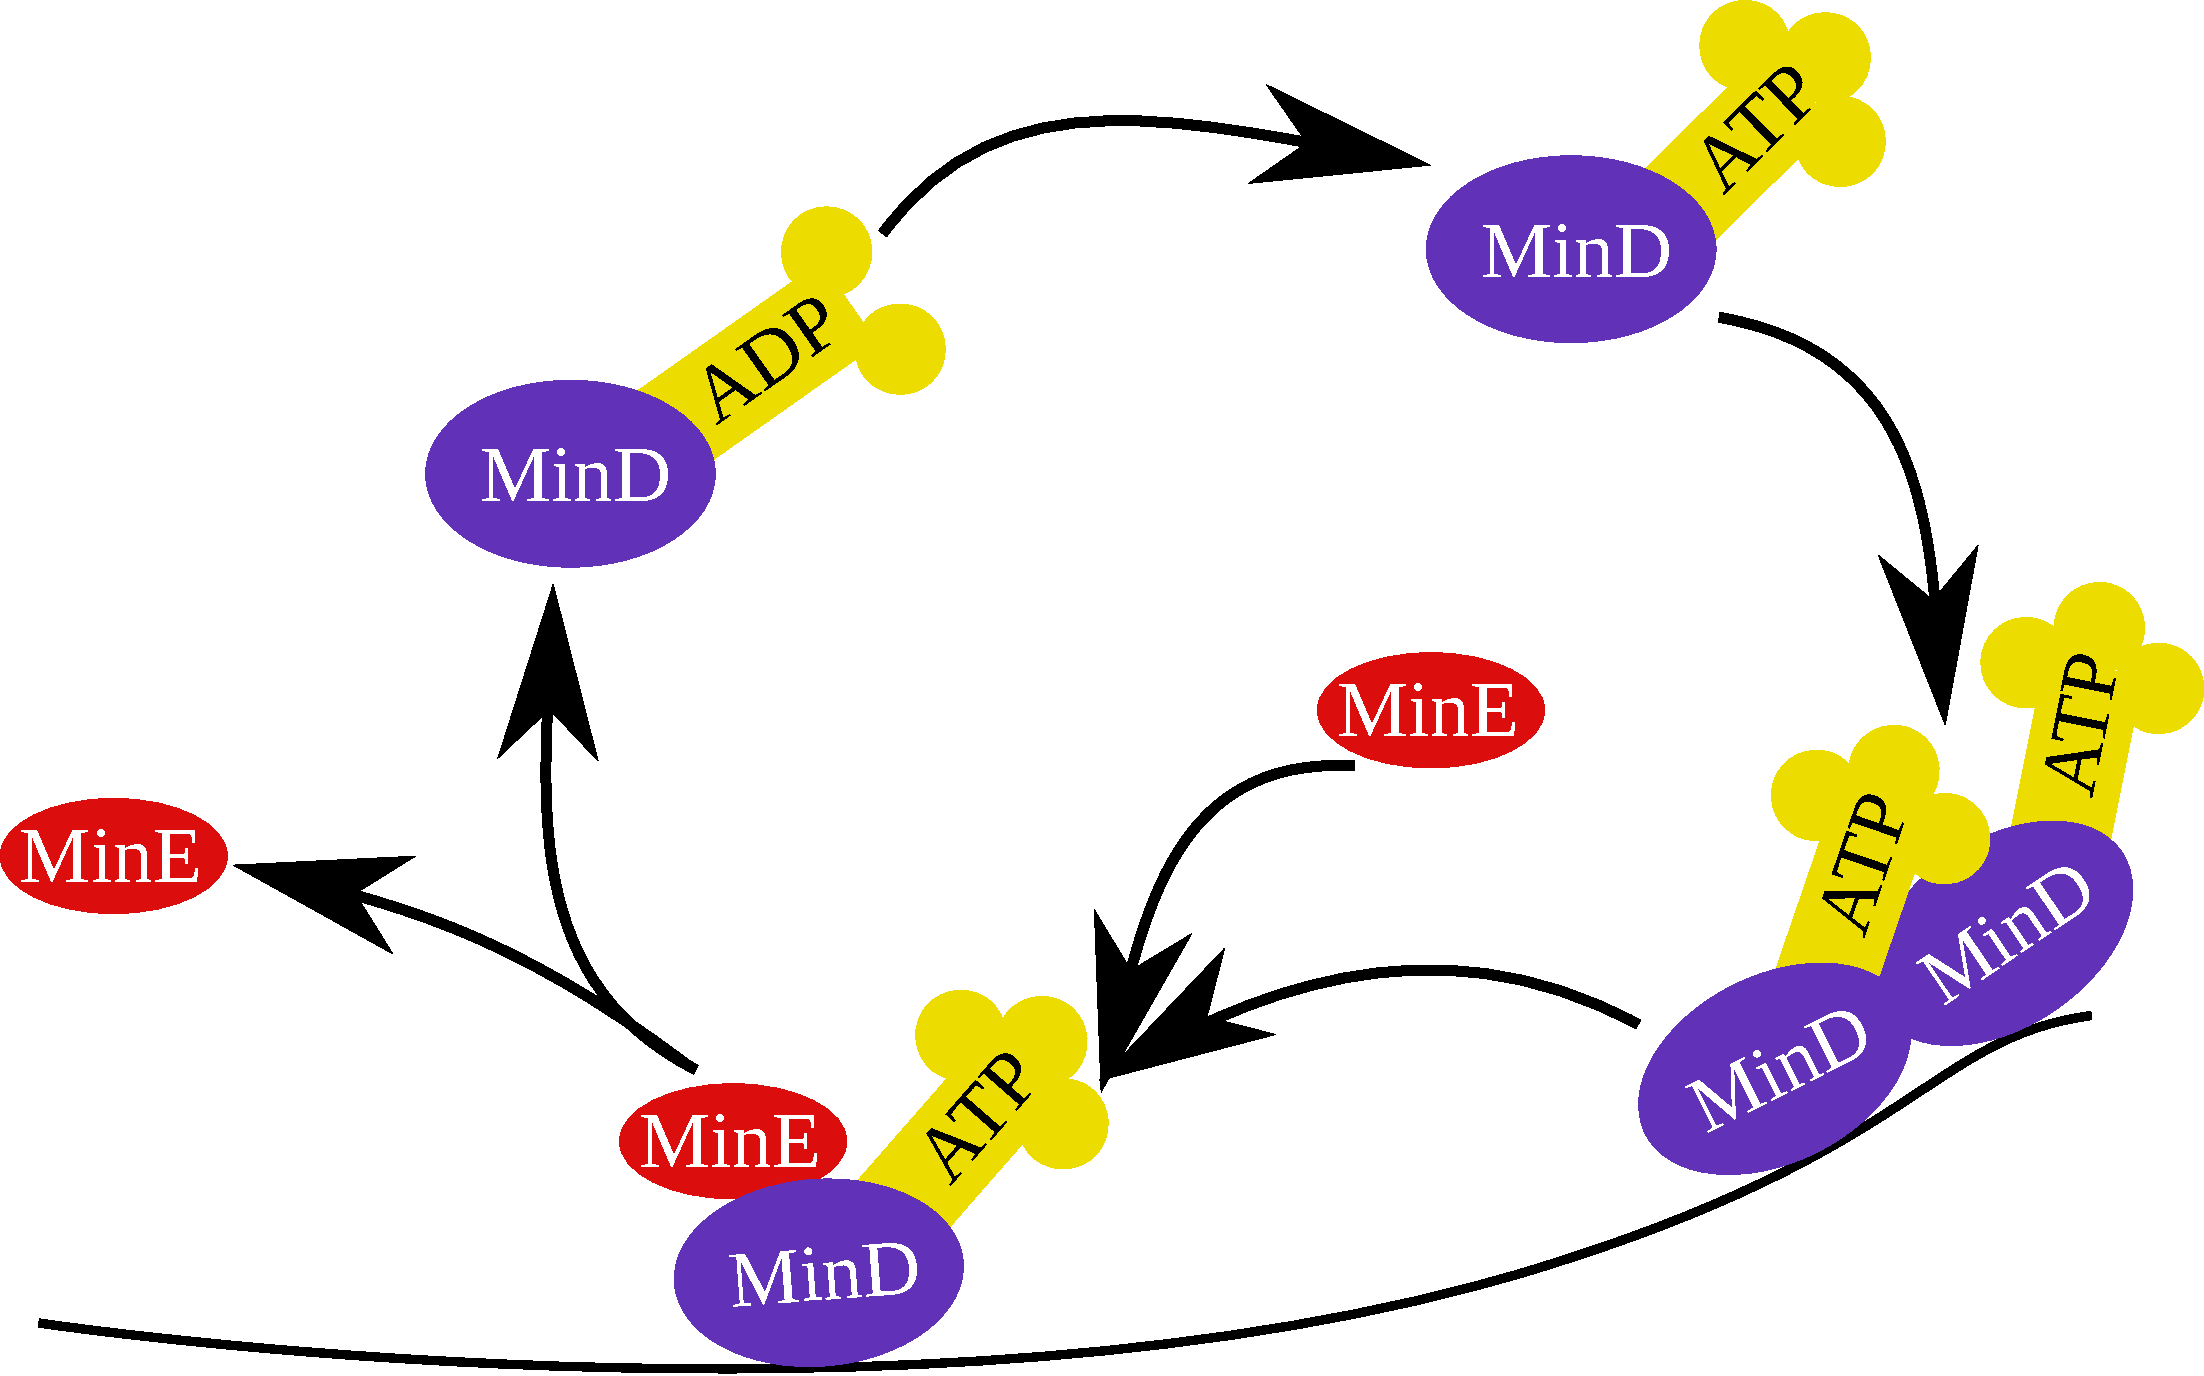
\includegraphics[width=\columnwidth]{reactions}
  \caption{Reactions included in the model of Huang \emph{et
      al.}~\cite{huang2003dynamic}.}\label{fig:reactions}
\end{figure}


\section{Model, Methods, and Cell Shapes}\label{sec:model-method-shapes}
We implement the reaction-diffusion model of Huang \emph{et
  al.}~\cite{huang2003dynamic}.  Figure~\ref{fig:reactions} shows the
reaction process.  The cytoplasmic MinD:ADP complex undergoes
nucleotide exchange and is changed into the MinD:ATP complex.  This
will naturally diffuse and attach to the cell membrane.  A cytoplasmic
MinE will attach to the wall bound MinD:ATP complex and after a time
will activate ATP hydrolosis.  This breaks up the complex, releasing
MinE, phosphate, and MinD:ADP back into the cytoplasm.  The MinD:ADP
will undergo nucleotide exchange and begin again the cyclic process.
The model is defined by a set of five reaction-diffusion equations:

\begin{multline}
  \frac{\partial \rho_{D:ADP}}{\partial t} = \mathcal{D}_D\nabla^2\rho_{D:ADP}-k_D^{ADP\rightarrow ATP}\rho_{D:ADP}\\
  +\delta(d_w)k_{de}\sigma_{DE},\hspace{3.4cm}
\end{multline}
\begin{multline}
  \frac{\partial \rho_{D:ATP}}{\partial t} = \mathcal{D}_D\nabla^2\rho_{D:ATP}+k_D^{ADP\rightarrow ATP}\rho_{D:ADP}\\
  -\delta(d_w)[k_D+k_{dD}(\sigma_D+\sigma_{DE})]\rho_{D:ATP}
\end{multline}
\begin{multline}
  \frac{\partial \rho_E}{\partial t} = \mathcal{D}_E\nabla^2\rho_E+\delta(d_w)k_{de}\sigma_{DE}
  -\delta(d_w)k_E \sigma_D \rho_E
\end{multline}
\begin{multline}
  \frac{\partial \sigma_D}{\partial t} = -k_E\sigma_D\rho_E
  +[k_D+k_{dD}(\sigma_D+\sigma_{DE})]\rho_{D:ATP}
  \label{eq:d-on-wall}
\end{multline}
\begin{multline}
  \frac{\partial \sigma_{DE}}{\partial t} = -k_{de}\sigma_{DE}+k_E\sigma_D\rho_E\hspace{3cm}
  \label{eq:FifthPDE}
\end{multline}
where $\rho$ is cytoplasmic protein density (proteins$/\micron^{3}$), $\sigma$
is membrane bound density (proteins$/\micron^{2}$), $\mathcal{D}_D$ and
$\mathcal{D}_{E}$ are the diffusions constants for MinD and MinE,
respectively, $k_D^{\textrm{ADP $\rightarrow$ ATP}}$ is the rate of
conversion from MinD:ADP to the MinD:ATP complex, $k_D$ is the rate of
MinD:ATP attachement to the membrane when no protein is already
attached there, $k_{dD}$ is the increase of this rate when MinD:ATP is
present on the membrane, $k_{de}$ is the rate of hydrolisis of the
MinD:MinE:ATP complex, $k_E$ is the rate of cytoplasmic MinE binding
to membrane bound MinD:ATP complex, and $d_w$ is the distance from the
point in space to the closest wall.  The Dirac delta function
$\delta(d_w)$, which we need to describe the location of the membrane,
has units of $\micron^{-1}$ and is zero everywhere except at the wall.
Equations \ref{eq:d-on-wall} and \ref{eq:FifthPDE} are only relevent
at the membrane because the membrane-bound density values have no
meaning in the cytoplasm.

Our diffusion and reaction rates are shown below.  We are interested
primarily in the effect of cellular size and shape on the protein
oscillations, so we follow Huang\cite{huang2003dynamic} and do not
deviate from the wild-type values used in the cited work.

\begin{gather*}
  \mathcal{D}_D = \mathcal{D}_{E} = 2.5\micron^2/\text{sec}\\
  k_D^{\textrm{ADP $\rightarrow$ ATP}} = 1/\textrm{sec,  }
  k_D = 0.025 \micron /\textrm{sec}\\
  k_{dD} = 0.0015 \micron^3/ \textrm{sec,  }
  k_{de} = 0.7/\textrm{sec}\\
  k_E = 0.093 \micron^3 /\textrm{sec}.
\end{gather*}

Huang's simulations use total MinD and MinE concentrations of
$1,000/\micron$ and $350/\micron$, respectively, in a cylindrical cell
of radius $0.5\micron$, and in our (non-cylindrical) cells we use the
same number of proteins per unit volume.  These concentration values
are $1273\micron^{-3}$ and $446\micron^{-3}$, respectively. We perform
simulations with a 3D grid in cartesian coordinates that has a grid
spacing of .05\micron.

We have performed both a numerical, deterministic model simulation
that is spatially and temporally discrete, and a stochastic simulation
that is spatially discrete but continuous in time.  Our stochastic
model follows the work of Kraus~\cite{kraus1996crosstalk} which in
turn follows a method introduced by
Gillespie~\cite{gillespie1977exact}.

We mean to investigate the geometric limits of the Min system
oscillations as observed by Mannik \emph{et
  al.}~\cite{mannik2012robustness}, so we have modeled the Min system
in several cell shapes and sizes.  Here we present a selection of
these, beginning with naturally occuring pill-shaped cells, followed
by a number of flattened out shapes which reflect the experiments of
Mannik \emph{et al.}, in which bacteria are confined within a thin
slit of height $0.25\micron$ ~\cite{mannik2012robustness}.  Viewed
from the top down the cells have the shapes described below and viewed
from the side they have at their edges a semicircular protrusion (one
may imagine the shape of a pancake).
%
In this paper we focus on four specific flattened cell shapes.  Two of
these shapes replicate those published by Mannik, and the other two
are `stadium' shapes that respectively have the same aspect ratio,
thickness, and volume as the two Mannik shapes.  Viewed from the top
down, these stadium shapes appear as rectangles with semi-circular end
caps on the long axis ends.

%% Our pill shapes differ from those of Huang \emph{et al.} in that they
%% are cylinders with hemisphere endcaps instead of pure cylindrical
%% shapes.  Our cylinderidrical radius is $0.5\micron$ and the lengths
%% of our cells (measured between the tips of the endcaps) are
%% $5\micron$, $4\micron$, $3\micron$, and $2.5\micron$.

%% \fixme{Is the following Kubitscheck paragraph needed?}
%% Kubitschek has shown in multiple experiments that at the time of cell
%% division cells have a volume that is within a range of roughly
%% $1\micron^3$ to $2\micron^3$~\cite{kubitschek1990cell,
%%   kubitschek1968linear}.  We follow Huang's
%% simulations\cite{huang2003dynamic} and Mannik's experiments and model
%% cells that are slightly larger than this range.

\begin{figure*}
  %\includegraphics[width=\textwidth]{../data/shape-p/3_00-0_50-0_00-0_00-15_00-exact/plots/image-plot}
  \begin{center}
    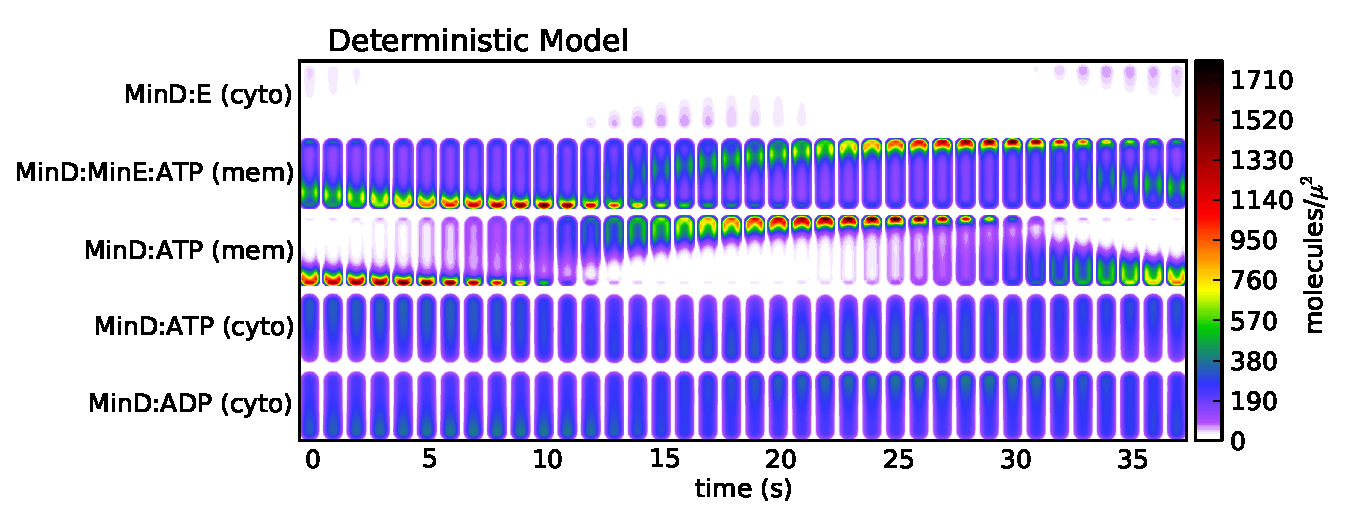
\includegraphics[width=0.8\textwidth]{determ-single-image-plot}\\
    \vspace{-1.5em}
    \includegraphics[width=0.8\textwidth]{stoch-single-image-plot}
    \vspace{-3em}
  \end{center}
  \caption{Images of the concentration of each protein species in a
    natural pill-shaped bacterium at one-second time intervals. The
    upper plots shows results from the deterministic model and the
    lower shows results from the stochastic model.  The order of
    frames is such that individual MinD proteins begin at the bottom
    of the plot (in the MinD:ATP state in the cytoplasm), and progress
    upward until they reach the MinE:MinD:ATP membrane-bound complex.
    At that point, they will spontaneously dissociate into cytoplasmic
    MinE (the top row) and the starting state of cytoplasmic
    MinD:ADP.}.
  \label{image-p}
\end{figure*}

Huang \emph{et al.}~\cite{huang2003dynamic} has performed a linear
stability analysis on a cylindrical model which shows an upper limit
on a steady state solution of a $2\micron$ half wavelength.  Cells
with dimensions longer than this show spontaneous oscillatory behavoir
in this direction, while cells that are shorter relax into a
motionless steady state.  We have similarly performed a linear
stability analysis on an infinite slab with a thickness equal to that
of our flattened cells ($0.25\micron$) and have found that an
equivalent stability limit for half wavelength is $2.13\micron$. As
expected, when decreasing the lengths and widths of our simulated
flattened cells so that the longest distance across the cell is less
than this length, the cells stop exhibiting any oscillatory behavior.
The deterministic model relaxes into a motionless state and the
stochastic model exhibits random fluctuations without spatial
oscillations.

\section{Naturally Occuring Pill Shaped Cells}

We begin with the naturally occuring pill cell shape.  We piece this
shape together as a cylinder with hemispherical endcaps.  This shape
follows the early simulations of Huang \emph{et al.} but differs in
that we have added the end caps for a more natural shape, expecting
similar results.

Figure~\ref{image-p} shows a series of color plots of the density of
proteins at each stage of the reaction cycle. Deterministic simulation
data is shown above and stochastic simulation data is shown below.
The cells shown are $4\micron$ in length, measured from end to end.
We have `smeared out' the stochastic concentrations in a manner meant
to reproduce the images shown by diffraction limited flourescence
microscopy.  We do so using the two dimensional gaussian approximation
developed by Zhang \emph{et al.}~\cite{zhang2007gaussian}.  In this
approximation we use a numerical aperture value of 1.3, which is the
same as used by Mannik experimentally, and a wavelength of $650nm$.
Each frame is 2.5 seconds ahead of the last, and each image shows the
concentration of a given state of protein (of the five described in
the reaction model) summed over the coordinate normal to the page.

Figure~\ref{image-p} begins about 300 seconds into the simulation and
shows one period of oscillation.  At $t=0$ there is a high
concentration of MinD:ATP that has accumulated on the membrane at the
bottom of the cell. An important aspect of Huang's model is that the
MinD is attracted to and sticks to the membrane nonlinearly: as it
accumulates there it begins to `recruit' other MinD that is diffusing
in the cytoplasm nearby, causing peaks in concentration to build up on
the walls.  Meanwhile, the MinE creeps downward as it reacts with the
membrane-bound MinD, forming the MinD:MinE:ATP complex, then breaks it
apart and diffuses downward a bit more before it again reacts with
membrane-bound MinD.  This process can be seen in the form of the
well-known ``MinE rings'' (actually, MinE bound to MinD on the
membrane).  These rings are visible in the deterministic model plots
as a green band on the walls from 0 seconds to 4 seconds (and later
from 15 to 23 seconds).  The appearence of these rings in the
deterministic model along side their less obvious appearence in the
stochastic model highlights an advantage of the deterministic model:
the idealization of deterministic data allows one to see patterns in
the averaged behavior that might otherwise be missed.  In the
stochastic model the MinE still exhibits higher concentrations in the
same regions throughout the process, but what would ideally be a
``ring'' pattern is instead an asymmetric collection of maxima, which
would become a ring after phase-locked averaging.

During the formation of these rings, cytoplasmic MinE is diffusing in
the upper portion of the cell and will naturally progress downward,
where there is membrane-bound MinD to react with, leading to a
depletion of MinE in the upper portion of the cell.  As the MinE ring
converges upon the lower end of the cell, MinD that has been released
is able to diffuse upward, past the ring, while still in its MinD:ADP
state and unable to bind to the membrane.  After it undergoes
nucleotide exchange, resulting in MinD:ATP, it is ready to accumulate
on the walls in at the top of the cell, where the MinE has been
depleted.  This can be seen in seconds 10 through 20 in both models,
followed by the subsequent MinE ring formation and movement upward
(beginning the same process in the opposite direction) that can be
seen in seconds 15 through 23.


%% is concentrated in the
%% upper portion of the cell and is diffusing downward, where it will
%% react with and stick to wall-bound MinD that is concentrated on the
%% membrane in the lower portion of the cell.  This process is in fact
%% already well on its way, as seen by the significant concentration of
%% wall bound MinD:MinE which is creeping down to the lower corner,
%% removing the MinD from the membrane as it goes.  The removed MinD
%% (cytoplasmic MinD:ADP) diffuses freely for a time before spontenously
%% undergoing nucleotide exchange and shifting back into the MinD:ATP
%% that is able to attach to the membrane.  Diffusing a small distance
%% away from the bottom of the cell will bring the protein into the MinE
%% \fixme{collection ??}, where reactions will prevent it from collecting
%% for any significant time on the membrane.  Diffusing further towards
%% the upper end, however, while the MinE has not yet collected there,
%% will allow MinD:ATP to accumulate with the other MinD:ATP, which is
%% seen at seconds 10 through 15 in Figure~\ref{image-p}.  Eventually the
%% MinE creeps all the way down to the bottom of the cell where it slowly
%% runs out of wall bound MinD to react with, before diffusing back up
%% and starting again on the upper portion of the cell. This is seen in
%% seconds 15 through 20 in the figure.  \fixme{There is another
%%   paragraph after this in the latex that I commented out because I
%%   thought we might be spending too much time on the description}

%%  At 15 seconds, the membrane-bound MinD:ATP has
%% been essentially removed from the top end of the cell, and MinD:ATP
%% has begun to bind to the membrane in the the lower half of the cell.
%% At this stage, there is a high concentration of cytoplasmic MinE at
%% the top of the cell, and by 16 seconds we begin to see the formation
%% of a MinE ring just below the center of the cell.  At 18 seconds, the
%% cell has reached its original state (reversed directionally), with
%% MinD:ATP bound to the membrane on the lower third of the cell, a high
%% concentration of cytoplasmic MinE in the upper half of the cell, and a
%% MinE ring pushing downward on the membrane-bound MinD:ATP.

\begin{figure}
  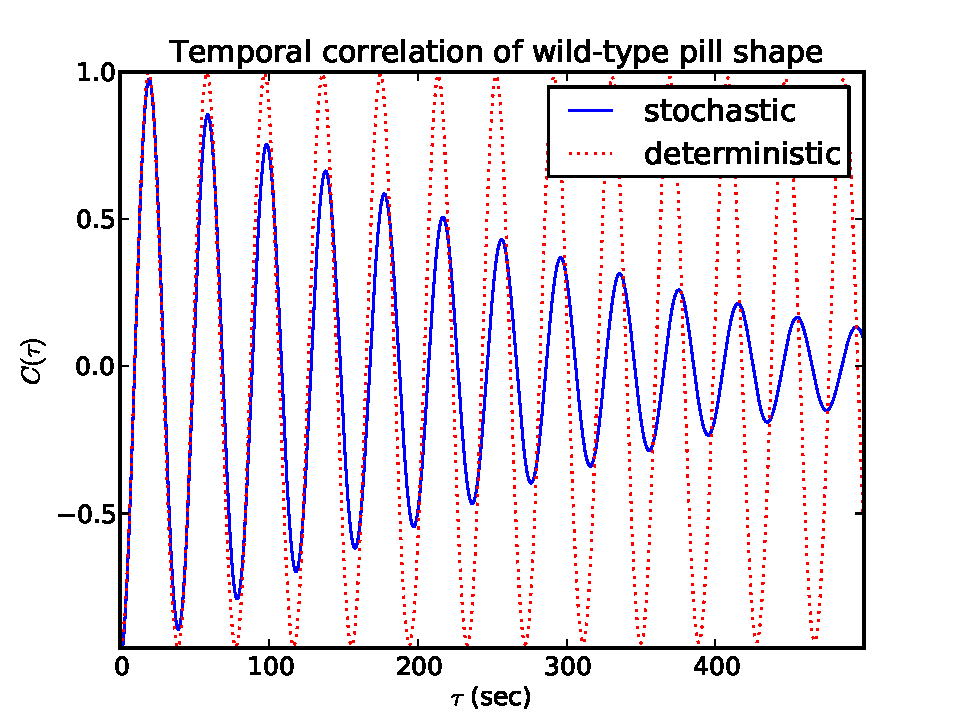
\includegraphics[width=\columnwidth]{pill-correlation.pdf}
  \caption{Temporal correlation function of the total MinD found in
    two opposite polar regions of the pill-shaped cell, shown against
    the correlation time.  Data for both the the determinisitic and
    stochastic models are shown.  The stochastic model shows an
    oscillation period of 39.5 seconds and coherence time of 307 seconds.
    The correlation functions are scaled to have the same initial
    value.}
  \label{corr-pill}
\end{figure}

It is clear from Fig.~\ref{image-p} that the stochastic simulation
results in a protein distribution that is less spatially regular than
the deterministic model predicts.  In fact, when viewed as a movie
(see supplementary material), the stochastic model exhibits a ``starry
night'' effect, as recruitment leads to clusters of MinD forming on
the wall and then subsequently dissipating.  This naturally leads to
irregularity in the temporal periodicity of the system, which we
quantify by examining the temporal correlation function of the total
MinD found in two opposite polar regions.
%
This correlation function, which is displayed in Fig.~\ref{corr-pill},
is given by
\begin{equation}
  C(\tau) \propto \int
  (N_{\textit{top}}(t) - \bar N_{\textit{top}})
  (N_{\textit{bottom}}(t+\tau) - \bar N_{\textit{bottom}})dt
\end{equation}
where $N_{\textit{top}}(t)$ and $N_{\textit{bottom}}(t)$ are the total
MinD proteins in the top and bottom thirds of a cell.  These plots
help us in studying the periods and the regularity and stability of
oscillations.  These curves are well fit with a simple decoherence
model, given by the equation
\begin{equation}
  C(\tau) = -\cos\left(\frac{2\pi\tau}{T}\right) e^{-\frac{\tau}{\tau_c}}
\end{equation}
where $T$ is the period and $\tau_c$ is the coherence time.  In the
case of the stochastic model the pill exhibits coherence times of
about 8 periods and in the case of the determinisitic model oscillate
indefinitely with complete coherence, indicating that its behavior is
perfectly periodic.

\begin{figure*}
  \centering
  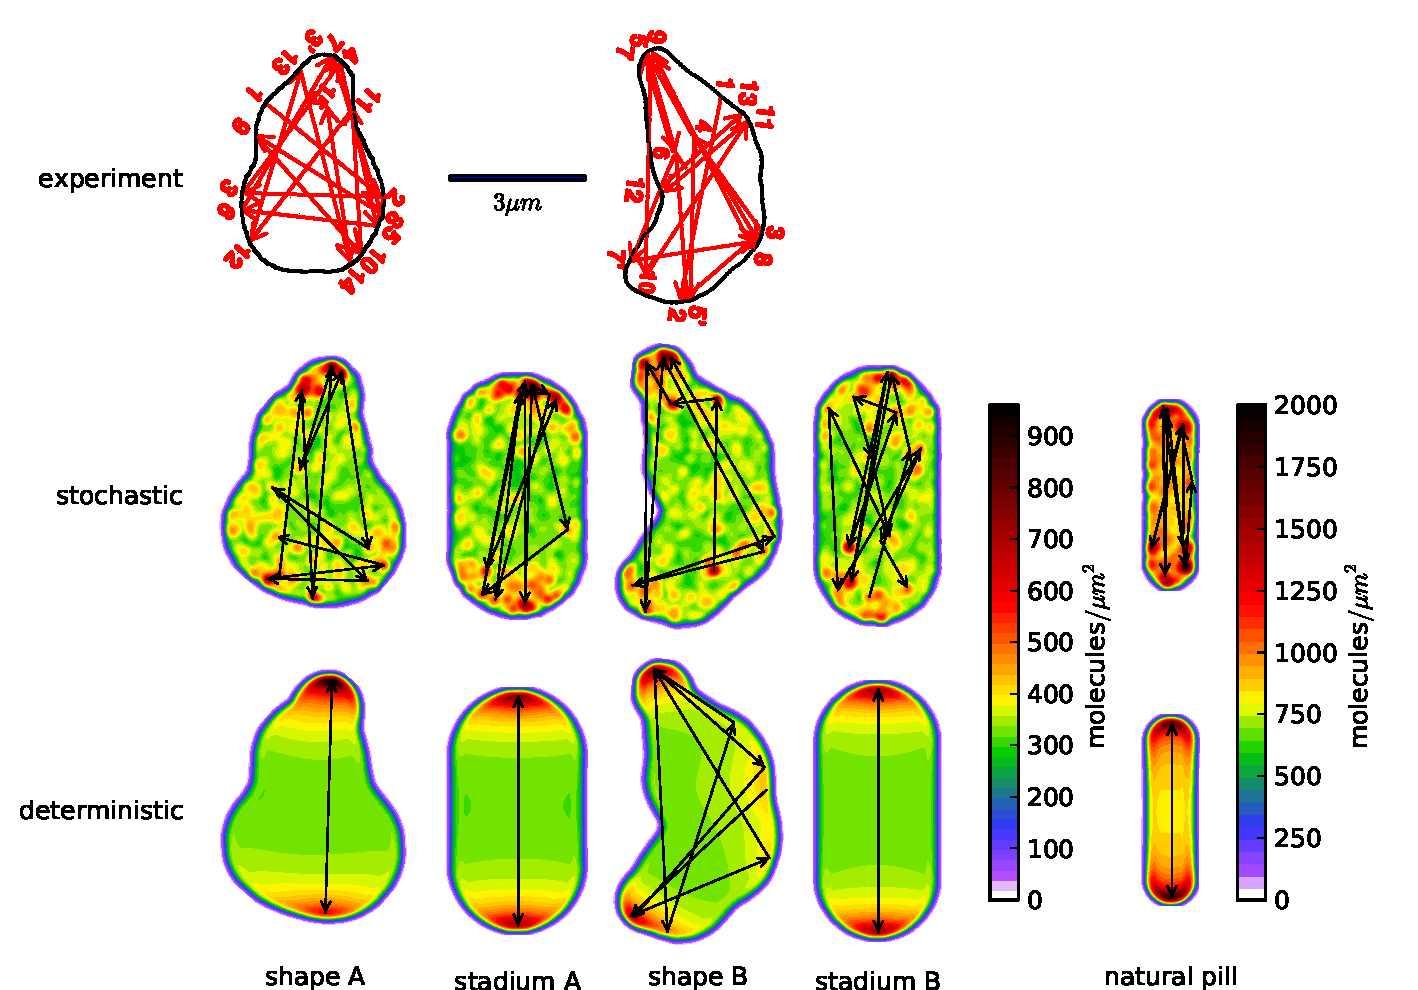
\includegraphics[width=0.8\textwidth]{plot-ave}
  \caption{We display here arrows depicting successive maxima in space
    and and time overlayed on a color plot of the total MinD density
    averaged over the same time period.  The simulation time covered
    for the flattened cells is 350 seconds, which is the same
    period of time depicted in the experimental data plots of Mannik
    \emph{et al.}~\cite{mannik2012robustness}.  For the wild-type pill
    shape, we only cover 250 seconds, in order to provide a
    useful comparison due to its shorter oscillation period.  The top
    row shows plots published by Mannik of the MinD maxima behavoir
    and the bottom two rows show our simulations using the stochastic
    and deterministic models, respectively.  We simulated
    approximations to the two shapes observed by Mannik, which we call
    \emph{shape A} and \emph{shape B}.  In addition, we studied two
    flattened stadium shapes which we call \emph{stadium A} and
    \emph{stadium B} corresponding in aspect ratio and thickness to
    the two experimental shapes.  The spatial length scale of all the
    figures shown was identical. Each of the flattened cell shapes
    uses the same color scale for the number of proteins per unit
    area.  Finally, we display the natural pill shape, which was also
    featured in Figs.~\ref{image-p} and~\ref{corr-pill}, with a
    different color scale to reflect the thicker cell containing more
    proteins per cross-sectional area.  }
  \label{randst-plot-ave}
\end{figure*}

\section{Comparison of Mannik's Experimental and Our Stadium Shapes}

As described in Section~\ref{sec:model-method-shapes}, we will focus
on simulation of four illustrative flattened cell shapes: two shapes
created to replicate those shapes observed experimentally by
Mannik~\cite{mannik2012robustness} (shape~\emph{A} and
shape~\emph{B}), and for comparison two symmetrical stadium shapes
that have the identical aspect ratio, thickness and volume (stadium
\emph{A} and stadium \emph{B}), shown in Figure~\ref{randst-plot-ave}.
These stadium shapes enable us to distinguish between the effect of
flattening the cell and the cell shape's irregularity and asymmetry.
We note that shape \emph{B} is more irregular than shape \emph{A}, and
in particular features a prominant region of concavity on its
left-hand side.  For each of these shapes (in addition to the
wild-type pill shape discussed previously) we have simulated in excess
of 15000 seconds (over 4 hours) of evolution of the MinD system using
the deterministic version of Huang's model~\cite{huang2003dynamic},
and in excess of 100000 seconds (over 27 hours) using the stochastic
model.

From each of these flattened simulations, we have chosen a typical 350
second segment to compare with the puplished results of
Mannik~\cite{mannik2012robustness}, exemplified in arrow plots in
which the arrow heads show the location of sequential MinD maxima
within the cell (in Fig.~\ref{randst-plot-ave}).  In addition to
arrows between successive maxima in space and time, we plot as a
colored background the density of MinD protiens averaged over the same
time period.  We note that we have manually verified that our
(computer-generated) arrow plots also reflect a human interpretation
of a movie of the same data.  Finally, for comparison we present the
same plot for a wild-type cell, with a time period of 250 seconds to
account for its short period of oscillation.

In every case, including the wild-type pill shape, we see irregularity
in the location of the maxima when using the stochastic model.  The
deterministic model shows uniformly bipolar oscillation, with the
exception of shape \emph{B}, which develops weak intermediate maxima
on the right-hand edge of the cell.  From these results, we conclude
that the deterministic model is inadequate to explain experimental
observations of the locations of density maxima of the MinD protein.


%% We found that the deterministic simulations of the MinD system results
%% in robust and regular oscillatory behavoir of polar selection and
%% oscillation in not only symmetrical shapes, such as the wildtype pill
%% shape, but also in very assymetrical, flatttened cells, such as those
%% observed by Mannik.  We also examined larger and smaller versions of
%% these shapes, and found this behavior to be very robust, from the
%% minimum size to sustain oscillation (around \fixme{???} $\mu$m) up to
%% around twice the cell size reported by Mannik.  At larger sizes than
%% this, less regular oscillations occur using the deterministic method,
%% but we note that the cells reported by Mannik are already considerably
%% larger in volume than typical wild type
%% cells~\cite{kubitschek1990cell,kubitschek1968linear,mannik2012robustness}.

\begin{figure}
  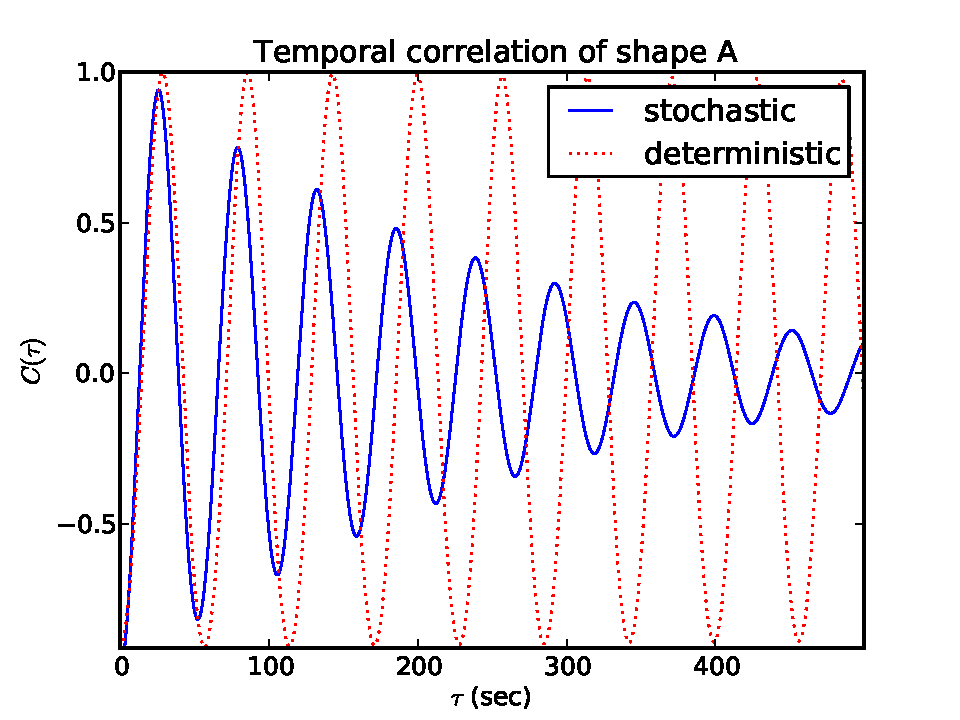
\includegraphics[width=\columnwidth]{shape-A-correlation.pdf}
  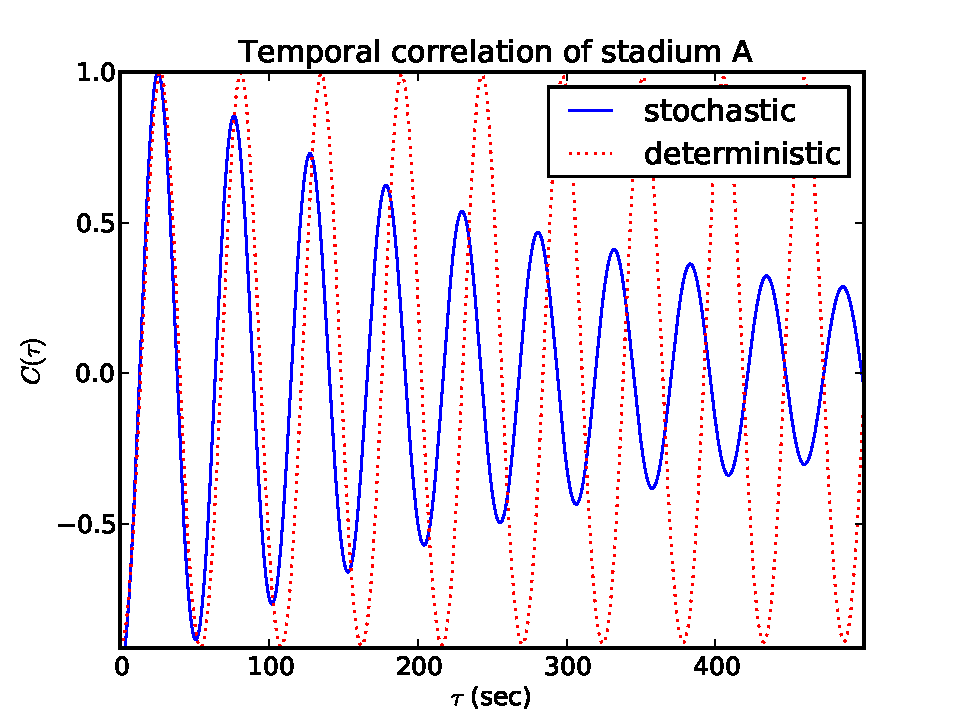
\includegraphics[width=\columnwidth]{stad-A-correlation.pdf}
  \caption{Temporal correlation function of the total MinD found in
    two opposite polar regions of the shape \emph{A} (above) and the
    stadium \emph{A} (below) cell shapes, shown against the
    correlation time.  Data for both the the determinisitic and
    stochastic models are shown, and the correlation functions are
    scaled to have the same initial value.  For shape \emph{A}, the
    stochastic model shows an oscillation period of 53.1 seconds and
    coherence time of 246 seconds, so that it takes roughly 4.6 periods
    for the behavoir to decohere.  For the stadium \emph{A}, the same
    model shows an oscillation period of 51 seconds and coherence time of
    323 seconds, so that it takes roughly 6.3 periods for the behavoir
    to decohere.}
  \label{fig:corr-pancake-A}
\end{figure}

The predictions of the stochastic model are roughly similar to the
experimental results in terms of irregularity of the locations of
maxima, although there are locations on the edges of the cells where
experiment shows maxima occuring that we never see in our simulations,
suggesting that the model does not precisely reflect the experiment.
We also note that the stadium shapes in Fig.~\ref{randst-plot-ave}
appear to have maxima location irregularity that is qualitatively
similar to our Mannik shapes and to experiment.

However Fig.~\ref{randst-plot-ave} leaves unclear the importance of
the flattening of the cell versus cell shape irregularity and
asymmetry in developing an understanding of the origin of the
experimentally observed behavior.  Although in the movies the stadiums
appear to display, on average over long time scales, a more regular
bipolar oscillation than the irregular mannik shapes, the limited time
range of the arrow plots (350 seconds) is inadequate when studying
this difference in behavoir.  We therefore return to the correlation
function between the number of proteins in a segment at the top of the
cell and the number of proteins in a segment at the bottom of the
cell.  Fig.~\ref{fig:corr-pancake-A} shows this plot for shape
\emph{A} and stadium \emph{A}.  E. Coli cell doubling times vary
widely depending on environmental conditions, but will often be
between 20 minutes to 100 minutes~\cite{pierucci1972chromosome}, while
flourescent microscopy experiments have shown that the FtsZ ring
builds itself with a half life of roughly 30
seconds~\cite{stricker2002rapid}.  Here we plot correlations of
correlation times up to 500 seconds, a biologically relevent
timescale.

%% \begin{figure}
%%   \includegraphics[width=\columnwidth]{../data/shape-randst/0_25-18_60-28_60-94_00-15_00-full_array/plots/correlation.pdf}
%%   \includegraphics[width=\columnwidth]{../data/shape-stad/0_25-2_92-1_18-0_00-15_00-full_array/plots/correlation.pdf}
%%   \caption{Correlation for B shapes}
%%   \label{corr-B}
%% \end{figure}

We see that both in the shape \emph{A} and stadium \emph{A}, the
deterministic model is perfectly periodic.  Both the deterministic and
stochastic model correlations have the same number of proteins in
their cells, and have been normalized with the same normalization
factor, so that they can be directly compared against eachother.  The
stochastic simulation of shape \emph{A} has a coherence time of 4.6
periods, while the corresponding simulation of stadium \emph{A} has a
coherence time of 6.3 periods.
%
The correlation function for stadium \emph{B} is similar to that of
stadium~\emph{A}, with similar coherence time (5.5 periods, not
shown), while shape~\emph{B} exhibits a lower coherence time (2.2
periods).  In the deterministic model, shape~\emph{B} is not precisely
periodic on biologically relevant timescales, which is reflected in
Fig.~\ref{randst-plot-ave}, in which the arrows describing the
deterministic model applied to shape \emph{B} show minor maxima
forming on the right-hand side of the cell, in contrast to the regular
polar maxima formed by shape~\emph{A} and the two stadiums.
%
From the stochastic correlation data, we conclude that irregularity of
shape has only a moderate affect on the temporal regularity of the
oscillatory behavior, with even the very distorted shape~\emph{B}
exhibiting only a factor of two greater decoherence.

\section{Conclusion}

We find agreement between our stochastic simulations and experiments
showing disrupted bipolar MinD oscillation in asymmetric flattened
E. coli cells~\cite{mannik2012robustness}.  As observed
experimentally, our simulations predict that MinD maxima will form in
a spatially irregular sequence of locations.  This result builds upon
existing results showing that this model is effective in a variety of
wild-type and mutated cell shapes~\cite{fange2006noise, varma2008min,
  kruse2007experimentalist}, and reinforces that the stochastic
variation of Huang's 2003 model~\cite{fange2006noise,
  kerr2006division} has considerable predictive power beyond the
standard wild-type cell.


%
%% We have simulated flattened cell shapes similar to those observed
%% experimentally by Mannik \emph{et al.}, with a stochastic and a
%% deterministic version of Huang's widely used reaction-diffusion model.
%% %
%% We find that the stochastic model predicts experimentally accurate
%% qualitative behavoir in both the wild-type, pill-shaped cells (as
%% found in previous studies~\cite{fange2006noise, varma2008min,
%%   kruse2007experimentalist}), as well as in the new, flattened,
%% irregularly shaped cells.  These flattened cells invariably show
%% spatially irregular formation of maxima as has been observed
%% experimentally.

In contrast to the stochastic model, the original deterministic
version of the model~\cite{huang2003dynamic} predicts behavior that
contradicts experimental observations, namely robust and periodic
bipolar oscillation in irregularly shaped cells, with a minor
intermediate maximum appearing in shape \emph{B}.  Thus we conclude
that this method is inconsistent with experiment, and cannot be relied
upon for predictions of the behavior of the MinD system.  This is the
most clear example of the inadequacy of the deterministic simulation
method in reproducing experimental behavoir of the MinD system to
date.  Until now the results of deterministic and stochastic
simulation have largely coincided, with the stochastic method showing
minor differences in behavoir when compared to deterministic
models~\cite{kerr2006division, fange2006noise, huang2004min,
  kruse2007experimentalist}.

We find that flattened but regular and symmetric cells exhibit MinD
oscillations that are qualitatively similar to the oscillations
observed experimentally (and in our simulation) in irregular and
asymmetric cells.  This demonstrates that asymmetry is not required in
order to induce spatially irregular MinD oscillations.  In addition,
the temporal regularity of oscillations is only moderately affected by
irregularity in the shape of flattened cells.  Thus we conclude
that it is the flattening of the cells rather than their irregular
shape that primarily causes the spatial irregularity of maxima which
is observed by Mannik \emph{et al.}~\cite{mannik2012robustness}.
%% %
%% In order to understand the irregular MinD oscillations observed in
%% experiments with flattened cells, we simulated flattened ``stadium''
%% shapes in order to distinguish between the effect of flattening and
%% the effect of irregular shape.
%% %
%% We found only a moderate difference in the coherence of bipolar
%% oscillations within these stadium shapes and the irregular shapes
%% observed by Mannik \emph{et al.}, and have observed visually the same
%% qualitative spatially irregular formation of maxima in both.  Thus we
%% conclude that the disruption of the MinD oscillations seen by Mannik
%% \emph{et al.}  is largely due to the flattening of the cell shape, as
%% opposed to its irregularity.

%% mannik B 11500 seconds, mannik A 15600 seconds, stadium A 19120  seconds, pill 19990 seconds
%% = simulation time that deterministic correlation data covers.


\clearpage
\newpage
\chapter{MinD Paper}
\input{protein-paper.tex}
\clearpage
\newpage
\chapter{Introduction to cDFT papers}

Talk about why need functionals to deal with inhomogenous situations.
Then talk about how functional deriviatives are taken.

\section{Classical Density Functional Theory}

A classical statistical ensemble is a collection of an arbitrary
number of classical systems of particles that have the same
macroscopic properties and internal restrictions, but have positions
and momenta that are otherwise distributed randomly.  In the canonical
ensemble, the number of particles $N$, the total volume of the system
$V$, and the tempurature $T$ are constant.  In this ensemble the free
energy, defined as $F = U - TS$, where $U$ is the internal energy and
$S$ is the entropy of the system, is at a minimum in thermodynamic
equilibrium. In the grand canonical ensemble, the number of particles
is allowed to vary while $V$, $T$ and the chemical potential $\mu$ are
constant.  In this ensemble it is the grand potential, defined as
$\Omega = F - \mu N$, that is at a minimum in thermodynamic
equilibrium.

In the case of inhomogenous fluids, a treatment of the inhomogenous
external potential $\phi(\rr)$ restricts the positions of the
particles in the system and stands in the place of the volume $V$ in
the thermodynamic equations.  In such a system, a change in the
internal energy is
\begin{align}
  \delta U = T\delta S + \int \rho^{(1)}(\rr)\delta \phi(\rr)d(\rr) + \mu \delta N
\end{align}
where $\rho^{(1)}$ is the 'one particle density'.
$\rho^{(1)}(\rr)d\rr$ is the average number of particles at $\rr$
within a volume $d\rr$.  One can calculate $\rho^{(1)}(\rr)$ by taking
the one-particle limit of the n-particle density of the grand
canonical ensemble,
\begin{align}
  \label{eq:n-particle-density}
  \rho_N^{(n)}(\rr^n)=\frac{1}{\Xi}\sum^{\infty}_{N=n}\frac{exp(N\beta \mu)}{\Lambda^3 (N-n)!} \
  \int exp(-\beta V_N)d\rr^{(N-n)}.
\end{align}
$\rho_N^{(n)}(\rr^n)$ has the general form of a statistical mechanical
probability, with an integration over possible states of Boltzmann
factors divided by the grand canonical partition function,
\begin{align}
  \Xi = \sum_{N=0}^{\infty}\frac{exp(N\beta\mu)}{h^{3N}N!}\int\int exp(\beta \mathcal{H})d\rr^Nd\mathbf{p}^N.
\end{align}
$V_N$ in Eq.~\ref{eq:n-particle-density} is the total interaction
potential between all of the particles in the system, and the spatial
integral is taken over all the potential positions of the particles
\emph{other} than the $n$ particles at positions $\rr^n$.  The
$exp(N\beta \mu)$ term accounts for the chemical potential's
regulation of the average number of particles in the system.  When
implementing density functional theory, one adjusts $\mu$ in order to
restrict the system's average number of particles,
\begin{align}
  \int_{system} \rho_N^{(1)}(\rr)d\rr = \langle N \rangle
\end{align}
to be a desired value.

The probability density, which is closely related to the n-particles
density, is $f_0(\rr^N,\mathbf{p}^N;N)$.
$f_0(\rr^N,\mathbf{p}^N;N)d\rr^N$ is the probability that there are
$N$ particles in the system and that those particles are found within
the infinitesimal range of positions $\rr^N$ and momenta
$\mathbf{p}^N$.  It's definition is
\begin{align}
  \label{eq:prob-density}
  \mathit{f}_0(\rr^N,\mathbf{p}^N;N) = \frac{exp(-\beta(\mathcal{H}-N\mu))}{\Xi}
\end{align}
where $\Xi$ is once again the partition
function.

Classical Density Functional Theory assumes that the Hamiltonian can
be split into linearly combined parts:
\begin{align}\label{eq:hamiltonian}
  \mathcal{H}(\rr^N,\mathbf{p}^N) = K_N(\mathbf{p}^N) + V_N(\rr^N) + \Phi(\rr^N)
\end{align}
The three terms on the right are the kinetic energy, potential
interaction between particles, and external potential, respectively.
The kinetic energy is a function of only the momenta of the particles,
and the two potentials of only their positions.

Substituing this for the Hamiltonian term in Eq.~\ref{eq:prob-density}
and taking the natural logarithm, we have:
\begin{align}
  \label{eq:log-of-f}
  \ln \mathit{f}_0 = \beta\Omega - \beta K_N - \beta V_N - \beta \Phi_N + N\beta \mu
\end{align}
where we have used the relation
\begin{align}
  \Omega = -k_BT\ln\Xi,
\end{align}
which is the basic connection between thermodynamics and statistical
mechanics in the grand canonical ensemble.

Because the external potential $\Phi(\rr)$ and $\mu$ are both constant
and $\rho^{(1)}(\rr)$ is the average ensemble equilibrium density at
$\rr$, the two right most terms are
\begin{align}
  \langle \Phi_N \rangle = \int \rho^{(1)}(\rr)\phi(\rr)d\rr \
  and \
  \langle N\mu \rangle = \mu \int \rho^{(1)}(\rr) d\rr
\end{align}

Using these relations and switching terms around in
Eq.~\ref{eq:log-of-f} results in the equation
\begin{align} \label{eq:intrinsic-free-two}
  \langle K_N + V_N + k_BT \ln \mathit{f}_0 \rangle \
  = \Omega - \int \rho^{(1)}(\rr)\phi(\rr)d\rr + \mu \int \rho^{(1)}(\rr)d\rr
\end{align}

The thermodynamic definition of the grand potential gives us $F =
\Omega + \mu N$.  From this we can see that the right hand side of
Eq.~\ref{eq:intrinsic-free-two} is analougous to the free energy of
the inhomogenous system minus the energy due to the external
potential.  We call this function the 'intrinsic free energy' $\iF$
since it only includes the interaction energy between the particles
within the system:

\begin{align}
  \label{eq:intrinsic-free-three}
  \iF = \Omega - \int \rho^{(1)}(\rr)\phi(\rr)d\rr + \mu \int \rho^{(1)}(\rr)d\rr \
  = \langle K_N + V_N + k_BT \ln \mathit{f}_0 \rangle
\end{align}

It can be shown that for a given $\mu$, $T$, and defined function
$V_N$ describing the potential interaction between particles, there is
a one-to-one relation between the external potential function and the
equilibrium density profile $\rho^{(1)}$ at thermodynamic equilibrium.
The grand canonical density function $f_0$ (Eq.~\ref{eq:prob-density})
for a given function $V_N$, $\mu$, and $T$ is a function of only the
external potential, so as a result it is completely determined by
$\rho^{(1)}$.  $V_N$ is also wholly determined by $\rho^{(1)}$ and
$K_N$ is determined by tempurature.  Thus the right hand side of
Eq.~\ref{eq:intrinsic-free-three} is a function of only the external
potential and therefore also of only $\rho^{(1)}$, which means that
for a given $\mu$, $T$, and defined function $V_N$, $\iF$ is wholly
determined by $\rho^{(1)}$.

Thanks to all of this, we can write
\begin{align}
  \Omega_{\phi}[n] = \iF[n] + \int n(\rr)\phi(\rr)d\rr - \mu\int n(\rr)d\rr
\end{align}
where $n(\rr)$ is a density profile that we will adjust systematically
in order to minimize $\Omega_{\phi}[n]$.  When $\Omega_{\phi}[n]$ is
minimized, it becomes the minimized grand potential of the system, and
the density profile $n(\rr)$ of the system is the density profile in
thermodynamic equilibrium, $\rho^{(1)}$.  It is finding this density
profile in thermodynamic equilibrium, and then the properties that can
be derived from it, that is the ultimate goal of Classical Density
Functional Theory.  Throughout the rest of this dissertation I will be
using $n(\rr)$ to refer to the particle density of the system, and the
reader should understand that it is a function that is meant to be
adjusted in order to minimize the grand potential energy function.

We begin the process of Classical Density Functional Theory by
designing the functional form of the intrinisic free energy $\iF$.
This is the major theoretical part of the process.  We then decide
upon an external potential $\phi(\rr)$ that defines the external
restrictions of the system, set the tempurature $T$ and chemical
potential $\mu$, and systematically adjust the density profile until
we have found the global minimum of this grand potential.  I won't
discuss the process of finding the density profile that minimizes the
grand potential in this dissertation, primarily because the algorithms
that do this were all in place before I joined the lab!  My work is
centered around the first part of the process, namely constructing the
functional form of $\iF$.



\clearpage
\newpage



\section{Introduction to SAFT and explanation of first free energy term}

\fixme{do more of an introduction to SAFT, taken from papers}

Work on Classical Density Functional Theory for inhomogeneous fluids
involves creating the intrinsic free energy functional of the density
profile, $\iF[n]$.  This is comprised of a sum of terms that
individually address different conceptual aspects of the system.
Terms that treat different types of interaction between particles are
added to a term that describes the reference system.  The functional
that we use in our work is called the Statistical Associating Fluid
Theory or SAFT free energy, and it is broken into the following terms:

\begin{align}
  \iF_{SAFT} = F_{ideal} + F_{hard sphere} + F_{dispersion} + F_{association}
\end{align}
We will discuss the meaning of these terms below in much more detail,
but write it down now to illustrate the general structure of the total
functional.


Although we work specifically with the very popular SAFT functionals
in current development, our contributions described in the next
chapters are applicable to many different types of fluid functionals.
The next chapter details a function that we've created, the
distribution function at contact $g_\sigma(\rr)$, which treats
correlations between particles within a system, while the following
chapter discusses it's use within a specific SAFT functional and it's
effect upon that functional's results.  The chapter after that
introduces another function, the pair distribution function
$g^{(2)}_{HS}(\rr_1,\rr_2)$, that is closely related to the first.
It's important for the reader to recognize that while we discuss these
functions in terms of their place within the SAFT free energy, they
and their conceptual founding are useful to other Classical Density
Functional Theories.



The first two terms, $F_{ideal}$ and $F_{hard~sphere}$, are typically
thought of as the functional's reference system terms.  The
$F_{ideal}$ is ubiquitous, and treats particles that have no
interactions between them.  While the $F_{hard~sphere}$ term does
treat particle interactions, the type of interaction it treats is so
basic and simple that this term is also seen as a reference term and
is incorporated into many very different functionals.  I give a
detailed introduction to the particular functional that we use for the
$F_{hard~sphere}$ term below (that of the White Bear free energy),
because while we don't actually modify it in our implementation of
inhomogenous SAFT, we do draw heavily from its ideas when creating our
functions.  The rest of the terms in $\iF$ address different types of
interactions between particles.  SAFT itself departs from other
theories in these last two terms.  In inhomogenous fluids, each one of
these terms is itself a functional of the density profile.


The first term in the SAFT functional is the ideal free energy term
$F_{ideal}$, and it treats a system of particles that do not interact
with eachother.  This is an obvious place to start if one is to build
the description of particle interaction terms upon a reference system.
It's lack of interaction actually causes this term to be the only one
that we can construct exactly, with no approximations.  To see why, we
point out that a system of non-interacting particles is able to
satisfy what is usually called the the local density approximation
(although we shouldn't call it this here because for non-interacting
particles it's not an approximation!)  The idea is that the free
energy functional can be written as an integral of a completely local
function of the density profile:
\begin{align}
  \iF_{local~density}[n] = \int f(n(\rr)) d\rr
\end{align}
where $f(n(\rr))$ is the free energy per unit volume of a homogenoues
fluid at a density $n(\rr)$.  In essence, each bit of volume becomes
it's own thermodynamic system, with a free energy equal that of a
homogenous density of particles at the local density, and the free
energies from all the bits of volume are added up to get the total.
The construction neglects any interaction between the particles, so
that any spatial variation in the density will be due entirely to the
varying external potential.  As an approximation for interacting
fluids, it does in fact apply to external potentials that modulate the
density slowly over space, much more slowly than correlation lengths.
It has thus been used in the past to construct entire intrinsic free
energy functionals beyond the reference $F_{ideal}$ term (cite).  It
breaks breaks down rather quickly, however, near hard walls for
interacting systems, where often the spheres will stack up in 'layers'
(should see some figure) and the local densities become greater than
bulk freezing densities (cite).

However, $F_{ideal}$ can be constructed exactly in this integral of
local density fashion, so all we need to do is integrate the free
energy of an ideal homogenous system at the local density.  Going back
to basic thermodynamics and statistical mechanics, we have:
\begin{align}
  F = -k_BT \ln Q_N = -k_BT \ln (\frac{V}{N!\Lambda^3})
\end{align}
where $Q_N$ is the partition function and $\Lambda$ is de Broglie
thermal wavelength.  Using th Stirling approximation for $N!$, we have
\begin{align}
F^{id} = Nk_BT(\ln \Lambda^3 \rho - 1))
\end{align}
Taking this as the free energy per unit volume and integrating, we
have
\begin{align}
  F_{ideal}[n] = \frac{1}{\beta}\int d\rr n(\rr)(\ln (\Lambda^3 n(\rr))-1)
\end{align}
This will be our reference $F_{ideal}$ term, as is common within
Clasical Density Functional Theory.

\clearpage
\newpage

\section{Virial Equation, Mayer functions, and the Carnahan Starling Equation}

The second term in the SAFT intrinsic free energy functional,
$f_{hard~sphere}$, is generally refered to as a reference term and the
specific functional that we use for this term is also used in many
other density functional theories.  I'll introduce the functional and
the theory behind it in some detail in the next section because it is
so widely used and, more importantly, because an understanding of the
ideas involved is neccesary for an understanding of our own work.
Before describing the term itself, however, I'll explain in this
section some important things that lead up to this theory, namely the
Virial equation, Mayer functions, and the Carnahan Starling Equation.

The Virial Equation applies to homogeneous fluids.  It equates a
thermodynamic, intensive quantity (likes the pressure) to an expansion
of the homogeneous density of the fluid.  It's standard form is
\begin{align}
  \label{eq:virial-expansion}
  \frac{\beta P}{\rho} = 1 + \sum_{i=1}^{\infty}\beta_i\eta^i.
\end{align}
where
\begin{align}
  \eta = \frac{\pi \rho \sigma^3}{6}
\end{align}
is the 'packing fraction'.  $\sigma$ here is the diameter of the
spherical particles of the fluid.  The packing fraction is really just
a more convenient way to refer to the density, where we give each particle the volume of a sphere and think in terms of how much volume is taken up by particles as opposed to how many there are.  We use it extensively
throughout our work.

The expansion of Eq.~\ref{eq:virial-expansion} comes out of a
formulation of the partition function that is most often expressed as
a series of diagrams that have well defined rules of construction.  I
won't explain the diagrams or their rules here, but Figure(REF) shows
an example so that if the reader sees them somewhere she'll know what
they are.  A single term (or diagram) in this expansion of the
partition function is in fact a spatial integral of particle densities
multiplied by a number of what are called Mayer Functions.  I'll give
a loose outline of an explanation here, since a basic idea of where
this expansion comes from should be useful to the reader.  The
derivation starts with the partition function:
\begin{align}
  \Xi &= \sum_{N=0}^{\infty}\frac{exp(N\beta\mu)}{h^{3N}N!}\int...\int exp(-\beta \mathcal{H})d\rr^Nd\mathbf{p}^N \\
  &=\sum_{N=0}^{\infty}\frac{exp(N\beta\mu)}{h^{3N}N!}\int...\int exp(-\beta (V_N + \phi(\rr))d\rr^Nd\mathbf{p}^N
\end{align}
where $V_N$ is the interaction potential between all the particles in
the system and $\phi(\rr)$ is the external potential.  If the the
interaction potential can be written as a summation of pairwise
superposable interactions, i.e.
\begin{align}
  V_N = \sum_{i<j}^{all~particles} v(i,j)
\end{align}
 than the partition function can be written as
\begin{align}
  \Xi = \sum_{N=0}^{\infty}\frac{1}{N!}\int... \int \left(\overset{N}{\underset{i<j}{\Pi}} f(i,j)\right)
  \left( \overset{N}{\underset{i=1}{\Pi}} \frac{exp(\beta (\mu - \phi(\rr)))}{\Lambda^3}\right)d\rr^N
\end{align}
where $f(i,j)=exp(-\beta v(i,j))$ is the Mayer function between two
particles.  With the help of the diagrams, one can take the natural
logarithm of the partition function to get the grand potential, and
then derivatives to find what are called direct correlation functions
(which I won't explain here). The use of an identity yields a
relationship between the chemical potential and the density,
\begin{align}
  \beta \mu = \beta \mu^{id} - \sum_{i=1}^{\infty}\beta_i\rho^i.
\end{align}
Then the use of the relation from thermodynamics,
\begin{align}
  \left(\frac{\partial P}{\partial \rho}\right)_T \
  = \rho \left(\frac{\partial \mu}{\partial \rho}\right)_T,
\end{align}
allows one to express the pressure as
\begin{align}
  \frac{\beta P}{\rho} = 1 + \sum_{i=1}^{\infty}\beta_i\eta^i
\end{align}
where
\begin{align}
  \label{eq:virial-coeff}
  \beta_i = (\frac{6}{\pi \sigma^3})^i B_{i+1}.
\end{align}

The virial formulation of thermodynamic properties is useful, but it
requires an expansion of coeffients, which can be a nuisance
computationally.  Carnahan and Starling (cite) were able to develop a
rule for coefficient generation that approximates
Eq.~\ref{eq:virial-coeff}, but that results in integers that one can
use to make a geometric series.  Written in its analytic form, this
series is a simple, easy to use, and accurate approximation of the
pressure in a homogenous fluid as a function of density (or packing
fraction $\eta$):
\begin{align}
  \frac{\beta P}{\rho}=\frac{1+\eta+\eta^2-\eta^3}{(1-\eta)^3}
\end{align}
It also yields the free energy in the form
\begin{align}
  \frac{\beta F^{ex}}{N}=\frac{\eta(4-3\eta)}{(1-\eta)^2}.
\end{align}
This equation is specifically very successful in predicting the
pressure of the homogenous hard sphere fluid at different densities.



\section{$F_{hard~sphere}$, Fundemental Meaure Theory, and White Bear}

\fixme{White Bear uses MCSL equation of state, which is the generalization to
the multi component mixture of hard spheres of the Carnahan-Starling
equation of state.}

We now return to analyzing the terms that make up the SAFT free energy:
\begin{align}
  \iF_{SAFT} = F_{ideal} + F_{hard~sphere} +  F_{dispersion} + F_{association}.
\end{align}

Remember that the $F_{ideal}$ term treats particles that do not
interact with one another.  In fact,
this one term addresses any aspect of the system that is
non-interactive, in the sense that every other term in $\iF_{SAFT}$ is
designed to specifically deal with a different type of potential
interaction among the particles.  Thus, $F_{ideal}$ is in a sense the
most basic reference term in the system.  However, as I've stated
above, the second term, $F_{hard~sphere}$, which I will describe here,
is also considered to be a reference system.

The potential interaction it describes is based on the fact that every
particle has at it's core a 'hard-core' repulsion to any other
particle.  In other words, as two particles approach each other in
space, there is a sudden, sharp spike in potential that prevents the
two particles from 'overlapping'.  The forces here can be complicated,
deriving from nuclear forces and the exclusion principle, but our
classical theories seek to approximate these in simple ways.

The hard sphere potential interaction is characterised by an
impenetrable spherical volume that is centered at a particles'
position.  The potential between two of these hard spheres
discontinuously jumps from zero to infinity when the spheres are a
distance apart that is equal to their combined radii:
\begin{align}
  v(r) &= \infty,~~ r < r_A + r_B \\
  &= 0,~~ r > r_A + r_B
\end{align}
where $r$ is the distance between the two particles, and $r_A$ and
$r_B$ are the radii of the two particles.  This hard sphere potential
that we use is not the only commonly used method for treating the
hard-core repulsion between particles.  The Leonard-Jones potential,
for example, another widely used potential energy description,
approximates the repulsion with a positive term porportional to
$\frac{1}{r^{12}}$


After deciding upon this form for the potential, one must turn to the
much more difficult step of designing an appropriate free energy
functional.  One of the first methods by which people attempted to
deal with these interactions, which is actually not limited to hard
spheres, was to modify the form of the local density approximation
free energy discussed above,
\begin{align}
  F_{local~density}[n] = \int f(n(\rr)) d\rr
\end{align}
to incorporate information about the particle densities immediately
surrounding each point.  They did this by redefining the density at
each point to be a convolution of the surrounding density with a
weighting function:
\begin{align}
  \label{eq:convolution-of-density}
  \bar{n}(\rr) = \int w(|\rr-\rr'|) n(\rr') d\rr'
\end{align}
and then using a function of this modified density as a weighting
function in the local density approximation formulation of the free
energy:
\begin{align}
  \iF[n] = \int \frac{f^{ex}(\bar{n}(\rr))}{\bar{n}(\rr)} n(\rr) d\rr
\end{align}
Eq.~\ref{eq:convolution-of-density} allows one to shape the nature of
the interaction indirectly, by changing the structure of the weighting
function.  For example, if one were to choose for the weighting
function the step function $\Theta(|\rr-\rr'|)$, than the modified
density would incorporate in an equal way all the density within a
sphere surrounding the particle.  A functional constructed in this way
would be a very oversimplified example of a weighted density
approximation.  Practical theories formulated in this manner become
very complicated.  We introduce it here so that the reader knows what
it is and also because the central idea described by
Eq.~\ref{eq:convolution-of-density} is used in Fundemental Measure
Theory, which we will now describe, as well.

Fundamental Measure Theory (FMT), created by Rosenfeld in 1989, also
defines the free energy in terms of a series of convolutions of
densities, but it is a considerable departure from the weighted
density approximation theories.  It is based on an involved derivation
worked out by Perkis and Yevik in (YEAR) of an equation of state for a
homogeneous fluid.  Like the derivation of the Virial Expansion and
Carnahan-Starling Equation discussed above, this derivation also dealt
with correlation functions and ultimately expressed thermodynamic
properties in terms of homogeneous density.  Rosenfeld compared this
theory with the derivations of another theory call Scaled Particle
Theory, which once again I will not explain but will say that it has
to do conceptually with a system of spheres and a growing cavity in
which they are not allowed to go.  He recognized that the density
sides of the Perkis-Yevick equations can be reformulated in terms of
densities and functions constructed to describe the geometric
properties of spheres.  Rosenfeld then discovered that for
inhomogeneous systems, he could write down the intrinsic free energy
in terms of convolutions of densities with these spherical functions
in such a way that the Percis-Yevik correlation equations were
reproduced in the limit of homogeneous density.  The derivation is
certainly an involved (and brilliant) one, and there is actually
another derivation to get to the same place introduced by \fixme{tarazona?}
in \fixme{year} that is thought by some to be more elegant.  However I don't
use any ideas that are directly pulled from these derivations in my
work, besides those that can be taken from the general characteristics
(spherical nature) of the resulting Free Energy functional.

The result of all this is an intrinsic free energy which has the form:
\begin{align}
  \label{eq:F-FMT-form}
  \iF_{hard~sphere}[n] = \int \Phi({n_i(\rr)})d\rr
\end{align}
The integrand $\Phi$ here is a local function of $n_i(\rr)$, which are
the non-local convolutions of density with sphere-like weighting
functions discussed above.  In FMT they are referred to as
'fundamental measures'.  They are defined as:
\begin{align}
  n_3(\rr) &= \int n(\rr') \Theta(\sigma/2 -\left|\rr - \rr'\right|)
  d\rr' \label{eq:FMn3} \\
  n_2(\rr) &= \int n(\rr') \delta(\sigma/2 -\left|\rr - \rr'\right|) d\rr' \\
  \mathbf{n}_{2V}(\rr) &= \int n(\rr') \delta(\sigma/2 -\left|\rr - \rr'\right|) \frac{\rr-\rr'}{|\rr-\rr'|}d\rr'
\end{align}
\begin{align}
  \mathbf{n}_{V1} = \frac{\mathbf{n}_{V2}}{2\pi \sigma}, \quad
  n_1 &= \frac{n_2}{2\pi \sigma} , \quad
  n_0 = \frac{n_2}{\pi \sigma^2} \label{eq:FMrest}
\end{align}
We can see the spherical nature of the theory by inspecting the $n_i$.
The $n_3(\rr)$ weighting function is a step function that is designed
so that the density is integrated over the volume of a sphere of
radius $\sigma/2$, but will make no contributions outside of this
sphere.  $n_2$ only allows for integration of densities on the surface
of a sphere, but incorporates no density within or outside of it.
$n_{2V}$ is a vector version of $n_2$, and the others are different
versions of the same, modified to have different units.

The form of $\Phi({n_i(\rr)})$ is restricted to a certain extent by
dimensional analysis (the units of each term have to be right!)
throughout the derivation, but even given this the theory allows for a
certain amount of freedom in it's design.  Since his derivation of FMT
was originally based on concepts in the Perkis-Yevik derivation of the
equation of state, Rosenfeld constructed the form of his functional so
that in the limit of homogeneous density, the free energy of the
system approaches that given by the Perkis-Yevik equation of state.

While the theory has been a resounding success (\fixme{MAYBE MENTION
  HOW SUCCESSFUL IN BEGINNING OF SECTION}, the use of the Perkis-Yevik
equation of state as the underlying, homogeneous limit equation causes
problems.  The construction of FMT obeys a theorem called the 'contact
value theorem,' which states that the pressure at a wall is equal to
the temperature multiplied by the density in contact with that wall,
$p=kTn_{contact}$. This theorem is very important in our own work, so
I'll discuss it in detail below.  I mention it here though because for
the hard sphere fluid, the Perkis-Yevik equation predicts a pressure
that is too high as bulk freezing tempuratures are approached.  It
consequently overestimates the density at contact at these
tempuratures.  This is problematic, since much of the reason we use
classical density functional theory in analyzing inhomogeneous fluids
in the first place is to estimate what happens at walls!

In (\fixme{year}) Roth et al addressed this issue in their version of FMT
which they named 'White Bear', anecdotally after a pub that they
frequented while writing the theory.  They keep the same general form
of Rosenfeld's FMT but adjust it so that in the limit of homogeneous
density it's free energy approaches that of the
Mansoori-Carnahan-Starling-Leland equation, a modified version of the
Carnahan-Starling equation of state, which we discussed above and
which we use directly in our own work.  The Carnahan-Starling is more
accurate in limiting cases than the Perkis-Yevik, so the White Bear
hard-sphere free energy functional, $F_{hard~sphere}$, is overall a
more accurate one.  It is therefore the hard sphere free energy
reference system that we choose to use in our own work.

Below is the entire energy functional written in terms of the
fundamental measure, $n_i(\rr)$:
\begin{equation}
F_\textit{hard~sphere}[n] = k_B T \int \left(\Phi_1(\rr) + \Phi_2(\rr) + \Phi_3(\rr)\right) d\rr \; ,
\end{equation}
with integrands
\begin{align}
\Phi_1 &= -n_0 \ln\left( 1 - n_3\right) \label{eq:Phi1}\\
\Phi_2 &= \frac{n_1 n_2 - \mathbf{n}_{V1} \cdot\mathbf{n}_{V2}}{1-n_3} \\
\Phi_3 &= (n_2^3 - 3 n_2 \mathbf{n}_{V2} \cdot \mathbf{n}_{V2}) \frac{
  n_3 + (1-n_3)^2 \ln(1-n_3)
}{
  36\pi n_3^2\left( 1 - n_3 \right)^2
} , \label{eq:Phi3}
\end{align}

\clearpage
\newpage

\section{Contact Value Theorem}
The contact value theorem is used directly in our own work and a
conceptual understanding of its origin will aid in the conceptual
understanding of the functions that we've created.  A derivation of it
is both justified and sort of awesome, so I dedicate this section to
it.

We start by considering a thermodynamic system of a fixed number of
particles.  The thermodynamic equations are:
\begin{align}
F &= U - TS \\
dU &= TdS -pdV \\
dF &= dU - TdS - SdT = -SdT - pdV.
\end{align}
The volume of our system will be fixed except for a tiny
(infinitesimally small) protrusion into it, jutting out from the wall,
illustrated in Figure(\fixme{reference}).  We will allow the protrusion to
either stick out or not, allowing the wall to either be flat and
smooth there or protruding.  We'll call the free energy in the two
different scenarios $F_{flat}$ and $F_{out}$, and investigate the
difference between them, or in other words what happens as the system
loses the bit of volume, dV.  The partition functions for these
scenarios are
\begin{align}
Z_{flat} &= \int_V... \int_V exp(-\phi \{\rr^N \})d\rr^N \\
Z_{out} &=  \int_{V-dV}... \int_{V-dV} exp(-\phi \{\rr^N \})d\rr^N
\end{align}
where $\phi \{\rr^N \}$ is the interaction energy between all the
particles and where we have ignored the kinetic energy terms, since in
both systems, which are at the same tempurature, these will be the
same \fixme{is this definitely true?}, and will later cancel out.  We
would like to write $Z_{flat}$ in terms of $Z_{out}$, so we'll
spatially break up the $Z_{flat}$ intagral.  The first term will
integrate over the same volume as $Z_{out}$.  The next set of terms
will treat the integration for one particle within the bit of volume,
interacting with all the other particles outside of the volume.  The
terms after that will integrate for two of the particles within the
bit of volume and all the remaining particles in the rest of the
volume.  The series will continue on in this fashion, with three
particles in the volume, then four, etc.:
\begin{align}
Z_{flat} = &\int_{V-dV}... \int_{V-dV} exp(-\phi \{\rr^N \})d\rr^N \notag \\
+ &\int_V... \int_V \int_{dV} exp(-\phi \{ \rr^N \})d\rr^N \
+ \int_V ... \int_{dV} \int_V exp(-\phi \{ \rr^N \})d\rr^N ... \notag \\
+ &\int_V... \int_{V}\int_{dV} \int_{dV} exp(-\phi \{\rr^N \})d\rr^N \
+ \int_V... \int_{dV}\int_V \int_{dV} exp(-\phi \{\rr^N \})d\rr^N ...
\end{align}
The term on the first line is just $Z_{out}$.  Looking at the next set
of terms, becuase every particle is identical it doesn't matter which
of them is within the little bit of volume.  Every one of these terms
will be the same, so they can be replaced by one of them multiplied by
$N$.  We will throw away the terms that are of higher order in $dV$,
and there are two arguments that allow us to do this.  The simplest
one is that $dV$ is small, and so terms with two $dV$s multiplied
together will be smaller.  One must be careful with this, however,
because the integration is really of the boltzmann factor over these
volumes.  If the interaction potential between the particles is
constructed so that they are highly attracted to eachother, than a
state in which there are two particles in the bit of volume can have
the same order of magnitude probability as the one in which there is
just one.  In this case we would not be able to say for certain that
these terms are so much smaller than the order one $dV$ terms that we
could reasonably ignore them. Thus the validity of the derivation
depends upon the size of the smallest measurement one can make along
the wall, and the nature of the attractive potential between the
particles.  In our case we deal with an interaction between hard
spheres, which simply exclude other spheres from being too close to
them.  Thus it's reasonable for us to imagine that if there is one
hard sphere in the bit of volume, than there is only the one, and any
terms that address the situation in which there are two in the bit of
volume can be ignored.  After applying these arguments we have:
\begin{align}
  \label{eq:zflat}
  Z_{flat} = Z_{out} + N \int_V... \int_V \int_{dV} exp(-\phi \{ \rr^N \})d\rr^N
\end{align}

Now we consider the statistical mechanical definition of the particle
density,
\begin{align}
  %%n(\rr) &= \frac{N \int_V... \int_V exp(-\phi \{ \rr^N \})d\rr^{N-1}}{\int_V... \int_V exp(-\phi \{ \rr^N \})d\rr^N} \\
  n(\rr) = \frac{N \int_V... \int_V exp(-\phi \{ \rr^N \})d\rr^{N-1}}{Z_{flat}}
\end{align}
Which is the sum of the boltzmann factors of all the states for which
a particle is at position $\rr$, divided by the partition function for
the system.  Comparing this with the right-most term in the
Eq.~\ref{eq:zflat} we see that:
\begin{align}
 N \int_V... \int_V \int_{dV} exp(-\phi \{ \rr^N \})d\rr^N  &= Z_{flat} \int_{dV} n(\rr) d\rr
 &\approx Z_{flat} n(\rr)dV
\end{align}
where on the right we make the approximation that because the volume
is small $n(\rr)$ is constant over it.
Thus we have
\begin{align}
Z_{flat} = Z_{out} + Z_{flat} n(\rr)dV \\
Z_{out} = Z_{flat} (1-n(\rr)dV)
\end{align}

Considering the change in the free energy when the system goes from a
flattened wall to a wall with a tiny protrusion, we have
\begin{align}
  dF = F_{out} - F_{flat} &= -kT \ln \left( \frac{Z_{out}}{Z_{flat}} \right) \notag \\
  &= -kT \ln \left( \frac{Z_{flat} (1-n(\rr)dV)}{Z_{flat}} \right) \notag \\
  &= -kT \ln \left( 1-n(\rr)dV \right) \notag \\
  &= kTn(\rr)dV
\end{align}
Then relating back to thermodynamics:
\begin{align}
  pdV &= dF = ktn(\rr)dV \\
  \label{eq:contact-value-theorem}
  p &= ktn(\rr)
\end{align}
Eq.~\ref{eq:contact-value-theorem} is the standard formulation of the
contact value theorem.


%% Another equation for the particle density is:
%% \begin{align}
%% n(\rr) = \frac{\delta \iF}{\delta V_{ext}}
%% \end{align}

\clearpage
\newpage

\section{Remaining terms in SAFT}
Going back to the terms in the overall SAFT free energy functional,
\begin{align}
  \iF_{SAFT} = F_{ideal} + F_{hard~sphere} +  F_{dispersion} + F_{association},
\end{align}
we come to introducing the last two terms.  These are actually the
only terms in which the functions that we've created show up, but
ironically I'll spend the least amount of time introducing them.  This
is because while the functions that we've created are included in
them, they could also be included in entirely different, non-SAFT
classical density functional theories, and their construction is
dependent on the concepts associated with the preceding terms, not of
$F_{dispersion}$ and $F_{association}$.


\clearpage
\newpage

\section{The convolution theorem}

Lastly within this introduction I will introduce a theorem, the
convolution theorem, that is a sort of important side note to the rest
of this text, primarily for the benefit of any new grad students that
might be entering this line of research in the future.  This theorem
motivates our preference of using density convolutions within our
functionals.

One of the largest advantages to using Fundamental
Measure Theory, and one that is not immediately obvious, is that the
convolutions that combine to construct the functional allow for very
efficient computation.  This is not very intuitive, since an integral
of a convolution integral must integrate over two dimensions, e.g.
\begin{align}
\int(f\ast g)(\xx)d\xx = \int \int f(\yy)g(\xx-\yy)d\yy d\xx
\end{align}
so that it may seem that the size of the computation would scale as
$N^2$, where $N$ is the size of the system.  It is true that in the
case of FMT, the weighting functions cut off the integrals at the size
on the order of a sphere of particle radius, but this can still be a
large enough volume so that a double integral for which one of the
volumes is this size and the other is the size of the whole system
would be too costly for practical computation.  FMT is saved, however,
by what is called the Convolution Theorem.  The Convolution Theorem
states that when one takes the Fourier Transform on a spatial
convolution of two functions (a double integral in space), the result
is two separate integrals over k-space that are simply multiplied
together:
\begin{align}
\hat{h}(\kk) = \hat{f}(\kk)\hat{g}(\kk)
\end{align}

When minimizing our functional, after
taking a Fourier Transform of the convolutions, we have merely to
integrate once over the one variable $\kk$.  Wait!  You may say.  This
is a cheat, since the Fourier Transform is itself an integral, so at
the end of the day we're still performing two integrals.  This would
be true if it were not for the computational technique known as Fast
Fourier Transforms, developed by (cite).  I won't explain how it works
here, but it's effect is to perform the transform, which would
normally have a computational cost on the order of N, with a
computational cost on the order of $\ln N$ instead.  Thus, when we
Fourier Transform the convolutions in the functional and proceed to
take the single integral over the result (in k-space), the
computational cost scales as $N \ln N$.  For large systems (we
simulate systems with hundreds or even thousands of particles) this
can certainly be the difference between practically possible and
impossible computations.  The proof is short and pretty so I'll relate
it here.

Say there is a function $h(\xx)$ such that
\begin{align}
  h(\xx) &= (f\ast g)(x) = \int f(\yy)g(\xx-\yy)d\yy
\end{align}
The fourier transforms are
\begin{align}
  \hat{f}(\kk) &= \int f(\yy) exp(-i2\pi \kk \cdot \yy)d\yy \\
  \hat{g}(\kk) &= \int g(\yy) exp(-i2\pi \kk \cdot \yy)d\yy.
\end{align}
and
\begin{align}
  \hat{h}(\kk) = \int h(\rr) exp(-i2\pi \kk \cdot \zz) d\zz &= \int \int f(\yy) g(\zz-\yy) exp(-i2\pi \kk \cdot \zz) d\yy d\zz
\end{align}
because the two integrals are taken over all space, we can say that if
\begin{align}
\xx &= \zz - \yy
\end{align}
than
\begin{align}
\hat{h}(\kk) &= \int \int f(\yy) exp(-i2\pi \kk \cdot \yy ) d\yy g(\xx) exp(-i2\pi \kk \cdot \xx) d\xx \\
&= \hat{f}(\kk) \hat{g}(\kk)
\end{align}



\clearpage
\newpage
\chapter{Contact Distribution Function}
\label{chapter:contact}
\newcommand{\red}[1]{{\bf \color{red} #1}}
\newcommand{\blue}[1]{{\bf \color{blue} #1}}
\newcommand{\green}[1]{{\bf \color{green} #1}}
%\newcommand{\rr}{\textbf{r}}
\newcommand{\refnote}{\red{[ref]}}

%\newcommand{\derivation}[1]{#1} % Use this to show all derivations in detail
\newcommand{\derivation}[1]{} % Use this for nice pegagogical paper...

% needsworklater is used to annotate bits that need work, but that we
% can postpone for a while.
\newcommand{\needsworklater}[1]{\emph{[#1]}}
% needsworknow is intended to prioritize stuff that needs fixing.
\newcommand{\needsworknow}[1]{\textcolor{red}{[\emph{#1}]}}
%\pacs{61.20.Ne, 61.20.Gy, 61.20.Ja}
%%%%%%%%%%%%%%%%%%%%%%%%%%%%%%%%%%%%%%%%%%%%%%%%%%%%%%%%%%%%
\section{Introduction}
In this chapter we discuss our investigation into the value of the
distribution function of an inhomogeneous hard-sphere fluid at
contact.  This quantity plays a critical role in SAFT.  We define two
averaged values for the distribution function at contact, and derive
formulas for each of them from the White Bear version of the FMT
functional, using an assumption of thermodynamic consistency. We have
tested these formulas, as well as two existing formulas against Monte
Carlo simulations, and have found excellent agreement between the Monte
Carlo data and one of our averaged distribution functions.

%%%%%%%%%%%%%%%%%%%%%%%%%%%%%%%%%%%%%%%%%%%%%%%%%%%%%%%%%%%%
% The following are papers that use a SAFT-based classical DFT with at
% least some of the terms purely local

A key input to the SAFT functionals is the distribution function
evaluated at contact, which is identical to the contact value of the
cavity correlation function for hard spheres, and is required for both
the chain and association terms in the SAFT free energy.

Yu and Wu introduced in 2002 a functional for the association term of
the free energy, which included a functional for the contact value of
the distribution function (described in
Section~\ref{sec:yuwu})\cite{yu2002fmt-dft-inhomogeneous-associating},
which has subsequently been used in the development of other
SAFT-based functionals\cite{fu2005vapor-liquid-dft, bryk2006density}.
%% Each of these terms has some dependence on the
%% inhomogeneity in the density.  The ideal gas is purely local, and in
%% fact must be the only purely local term in the free energy in order
%% for the functional to satisfy the contact-value theorem.  The
%% hard-sphere contribution contribution to the free energy has been
%% thoroughly studied, and is well approximated by the White Bear version
%% of the Fundamental-Measure Theory (FMT)
%% functional\cite{roth2002whitebear}.
Also, two functionals for the chain contribution have recently been
introduced, one which uses the
distribution function of Yu and Wu\cite{bryk2006density} and another which
introduces a new approximation for the contact value of the
distribution function\cite{gross2009density}.
%% The dispersion term is long-range and thus has significant
%% dependence on the density distribution, but because its relatively
%% weak position dependence, is amenable to mean-field approximations.
Here we will briefly describe how the contact value of the distribution
function has been used in two of these recent papers introducing
SAFT-based classical density functionals.  For simplicity, we will use
our own notation to describe the work of these authors.

In his paper
presenting a density functional based on the PCP-SAFT equation of
state\cite{gross2009density}, Gross introduces the chain free energy
in SAFT as
\begin{align}
  \frac{F_\textit{chain}}{kT} &= -(m-1) \int n(\rr) \left(\ln\left(n^A(\rr)
  g_\sigma^A(\rr) \right)-1\right) d\rr \label{eq:Achain}
\end{align}
where $n^A(\rr)$ is a weighted density defined as
\begin{align}
  n_A(\rr) &= \int n(\rr')
  \frac{\delta(\sigma -|\rr-\rr'|)}{4\pi\sigma^2} d\rr' \label{eq:nA}
\end{align}
and $g_\sigma^A(\rr)$ is the local value of the distribution function
at contact, which we define as
\begin{align}
  g^A_\sigma(\rr) &= \frac{1}{n(\rr)n_A(\rr)}
  \int n^{(2)}(\rr, \rr + \rr')
  \frac{\delta(\sigma -|\rr'|)}{4\pi\sigma^2}d\rr' \label{eq:gA}
\end{align}
In Section~\ref{sec:gross} we describe Gross's approximation for this
function.

In a paper describing a classical density functional for
inhomogeneous associating
fluids\cite{yu2002fmt-dft-inhomogeneous-associating}, Yu and Wu define
the association free energy as
\begin{align}
  \frac{F_\textit{assoc}}{kT} &= \sum_i \int \zeta(\rr)n_0(\rr) \left(\ln X_i(\rr) - \frac12
  X_i(\rr) + \frac12\right) d\rr \label{eq:Aassoc} \\
  X_i(\rr) &= \frac{1}{1 + \sum_j \frac{n_0(\rr) g_\sigma^{S}(\rr)}{\zeta(\rr)}
                                 X_j(\rr)\kappa_{ij} \left(e^{\beta
                                   \epsilon_{ij}}-1\right)}.
  \label{eq:X}
\end{align}
where $X_i(\rr)$ is the fraction of interaction sites of type $i$ at
position $\rr$ that are unoccupied, $n_0(\rr)$ is a weighted density
defined in Equation~\ref{eq:n0}, $\zeta(\rr)$ is a nonlocal measure of
the density gradient defined in Equation~\ref{eq:zeta}, and
$g_\sigma^S(\rr)$ is a form of the distribution function at contact,
which we define in Equation~\ref{eq:gS}.  In Section~\ref{sec:yuwu} I
present the approximation to $g_\sigma^S(\rr)$ introduced by Yu and
Wu.  Given these differing approaches, it seems valuable to examine
this property of the hard-sphere fluid through direct simulation, in
order to establish the advantages and disadvantages of each approach.

Although these recent works have introduced approximate functionals
for the contact value of the distribution function for an
inhomogeneous hard-sphere
fluid\cite{yu2002fmt-dft-inhomogeneous-associating, gross2009density},
there had not been a study that specifically addressed this
functional.
%
In our work we introduced two definitions for the locally averaged
distribution function of an inhomogeneous system.
%
%% The first is more symmetric (which we call the $S$ case), while the
%% second involves a sphere-centered, asymmetrical interpretation (the
%% $A$ case).
%
Given these definitions, I'll present a thermodynamic derivation for
each distribution function from the free energy functional.  We will
then discuss the distribution functions of Yu and Wu and of Gross, and
will end by comparing all four approximations with Monte-Carlo
simulations of the hard-sphere fluid at a variety of hard-wall
surfaces.


\section{Distribution function with inhomogeneity}

We define our terms using the two-particle density
$n^{(2)}(\rr_1,\rr_2)$, which gives the probability per unit volume
squared of finding one particle at position $\rr_1$ and the other at
position $\rr_2$.  The pair distribution function is defined by
\begin{align}
  g(\rr_1,\rr_2) &\equiv \frac{n^{(2)}(\rr_1,\rr_2)}{n(\rr_1)n(\rr_2)}
\end{align}
In a homogeneous fluid, the pair distribution only depends on the
distance $|\rr_1-\rr_2|$ and can be expressed as a function of a
single variable, and the contact value of the distribution function is
its value when evaluated at a distance of the diameter $\sigma$.  The
pair distribution function of an \emph{inhomogeneous} fluid is not as
simple, but it is desirable for reasons of computational efficiency to
construct classical density functionals using only one-center
convolutions.  Moreover, a local function is helpful when defining
functionals based on perturbation theory, such as those in
Equations~\ref{eq:Achain}-\ref{eq:X}.  This leads
us to seek a \emph{local} value for $g_\sigma$ that is dependent upon
only one position variable $\rr$.  There are two reasonable options
for defining such a local function: a symmetric formulation such as
that used in Equations~\ref{eq:Aassoc}-\ref{eq:X} (which we refer to
as $S$) and an asymmetric formulation such as that used in
Equation~\ref{eq:Achain} (which we refer to as $A$).

For the symmetric $S$ case, the distribution function at contact is
given by:
\begin{align}
  g^S_\sigma(\rr) &= \frac{1}{n_0(\rr)^2}\int n^{(2)}(\rr - \rr', \rr
  + \rr')
  \frac{\delta(\sigma/2 -|\rr'|)}{\pi\sigma^2}d\rr' \label{eq:gS}
\end{align}
where $\sigma$ is the hard sphere diameter and the density $n_0$ is one of
the fundamental measures of Fundamental Measure Theory (FMT).  The
functional $g^S_\sigma(\rr)$ is defined to treat the geometrically
symmetric possibility of spheres touching at the position $\rr$ as
illustrated in Figure~\ref{fig:n0}.
\begin{align}
  n_0(\rr) &= \int n(\rr')\frac{\delta(\sigma/2 -|\rr-\rr'|)}{\pi\sigma^2} d\rr'
  \label{eq:n0}
\end{align}
This functional $n_0(\rr)$ gives a density averaged over all spheres that touch at
the position $\rr$.  Together, $n_0(\rr)$ and $g_\sigma^S(\rr)$ are
used in the association free energy given in Equations~\ref{eq:Aassoc}-\ref{eq:X}.

\begin{figure}
\begin{center}
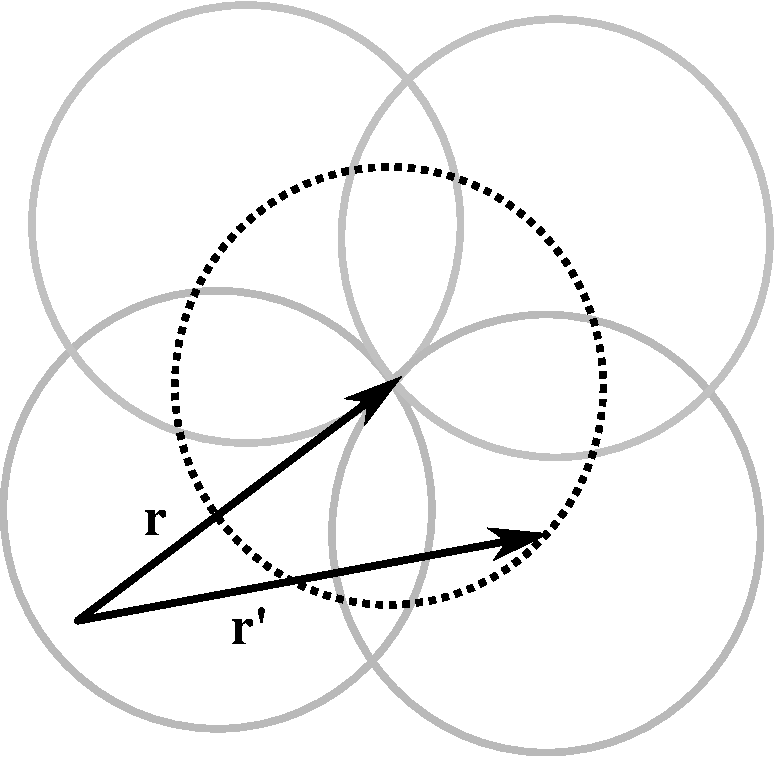
\includegraphics[width=5cm]{figs/n0}
\end{center}
\caption{Set of hard spheres that are included in $n_0(\mathbf{r})$, which
  consist of those which just touch the point $\mathbf{r}$.}
\label{fig:n0}
\end{figure}

\begin{figure}
\begin{center}
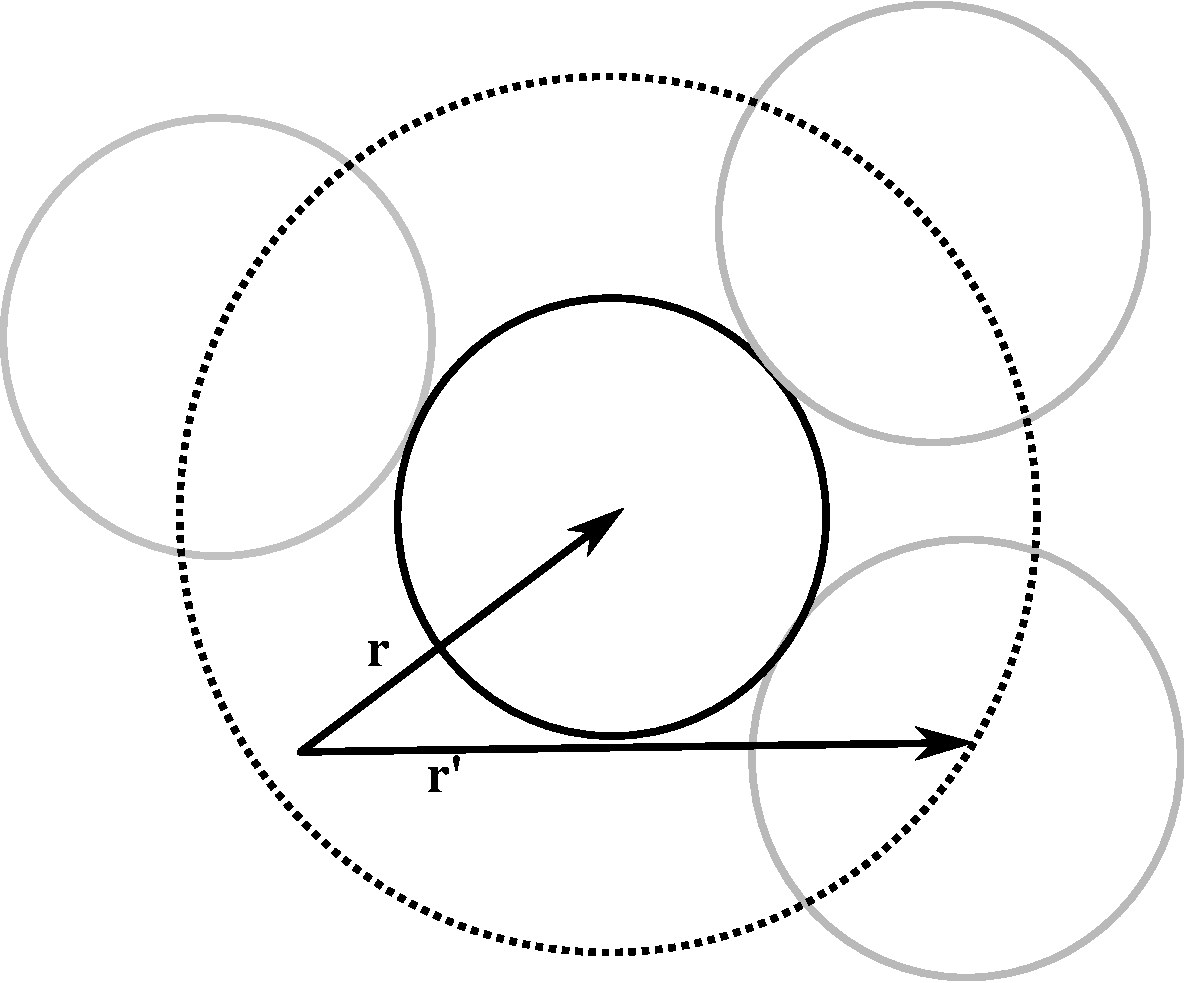
\includegraphics[width=7cm]{figs/nA}
\end{center}
\caption{Set of hard spheres that are included in $n_A(\mathbf{r})$,
  which consist of those which just touch a sphere centered at
  $\mathbf{r}$.  The dashed line illustrates the surface over which
  contact is possible.}
\label{fig:nA}
\end{figure}

In contrast, the asymmetrically averaged $A$ distribution function is
given by
\begin{align}
  g^A_\sigma(\rr) &= \frac{1}{n(\rr)n_A(\rr)}
  \int n^{(2)}(\rr, \rr + \rr')
  \frac{\delta(\sigma -|\rr'|)}{4\pi\sigma^2}d\rr' \label{eq:gA}
\end{align}
where the density $n_A(\rr)$ is analogous to $n_0(\rr)$, but measures the
density of spheres that are touching a sphere that is located at
point $\rr$, as illustrated in Figure~\ref{fig:nA}.
\begin{align}
  n_A(\rr) &= \int n(\rr')
  \frac{\delta(\sigma -|\rr-\rr'|)}{4\pi\sigma^2} d\rr' \label{eq:nA}
\end{align}
Thus $g_\sigma^A$ corresponds to an average of the two-particle
density over spheres touching a sphere that is located at the
position~$\rr$.  The functionals $n_A(\rr)$ and $g_\sigma^A(\rr)$ are
used in the chain free energy given in Equation~\ref{eq:Achain}.

%% In the process of defining these two averaged distribution functions,
%% we also defined two averaged densities, $n_0(\rr)$ and $n_A(\rr)$,
%% which are the density of spheres available to be in
%% contact.  In the homogeneous limit, $n_0 = n_A = n$.  It is an
%% open question, which of these averages will be more useful in any
%% particular functional.  Suffice to say, either average is a
%% \emph{possible} way to convert a function that is defined for a
%% homogeneous system to a functional that is applicable to inhomogeneous
%% systems.

%% Yu and Wu introduce an approximation for
%% $g^S$\cite{yu2002fmt-dft-inhomogeneous-associating}, which we will
%% discus in Section~\ref{sec:yuwu}.  Gross introduced an
%% approximation for $g^A$\cite{gross2009density}, which we will
%% introduce in Section~\ref{sec:gross}.  We will also introduce our own
%% approximations for both $g^A$ and $g^S$ which are based on the
%% assumption of thermodynamic consistency within FMT, in
%% Sections~\ref{sec:g-S} and~\ref{sec:g-A}.  We will report on the accuracy of
%% these approximations by comparing with Monte Carlo simulations of the
%% inhomogeneous hard-sphere fluid.  We will focus on the contact
%% densities, rather than the distribution function itself, because these
%% are simpler, and because they are the quantity that you want to
%% ``average''.  i.e. if you were to average $g$ itself, you'd want to
%% weight that average based on the density, which would mean averaging
%% $n^{(2)}$.


%% \subsection{Association free energy of SAFT}

%\fixme{Integrate the following equations into this section...}
%% \begin{align}
%%   \frac{A_\textit{chain}}{kT} &= -(m-1) n \left(\ln\left(n g_\sigma \right)-1\right)
%% \end{align}
%% \begin{align}
%%   \frac{A_\textit{assoc}}{kT} &= \sum_i n \left(\ln X_i - \frac12 X_i + \frac12\right) \\
%%   X_i &= \frac{1}{1 + \sum_j n g_\sigma X_j\kappa_{ij} \left(e^{\beta \epsilon_{ij}}-1\right)}
%% \end{align}

%% \newcommand\epsilonassoc{\ensuremath{\varepsilon_\textit{AB}}}
%% \newcommand\kappaassoc{\ensuremath{\kappa_\textit{AB}}}
\newcommand\ncontact{\ensuremath{n_\textit{contact}}}

%% The free energy term in Statistical Associating Fluid Teory (SAFT)
%% from which it derives its name is the association term, which accounts
%% for hydrogen bonding.  Hydrogen bonds are modeled as attractive
%% patches (``association sites'') on the surface of hard spheres.  These
%% sites represent protons or electron lone pairs, and have an attractive
%% energy $\epsilonassoc$ when two molecules are oriented such that the
%% proton of one overlaps with the lone pair of the other.  The volume
%% over which this interaction occurs is $\kappaassoc$, giving the
%% association term in the free energy has two empirical parameters fit
%% to experimental data.

%% The association free energy per unit volume has the form
%% \begin{align}
%%   f_\text{assoc} &= k_BT n\sum_A 
%%                   \left(\ln X^A - \frac{X^A}{2} + \frac12\right)
%% \end{align}
%% where the summation is over the association sites, and $X^A$ is the
%% fraction of association sites \emph{not} hydrogen-bonded.  The
%% fractions $X^A$ are determined by the self-consistent equations
%% \begin{align}
%%   X^A &= \frac{1}
%%   {1 + \sum_B n X^B \Delta^{AB}}\label{eq:X}
%%   \\
%%   \Delta^{AB} &= g(\sigma) \kappaassoc\left( e^{\epsilonassoc/kT} -
%%   1 \right)\label{eq:delta}
%% \end{align}
%% where $g(\sigma)$ is the distribution function evaluated at contact.
%% The product of density with distribution function evaluated at contact
%% gives the contact density, when we combine Equations~\ref{eq:X} and
%% \ref{eq:delta}:
%% \begin{align}
%%   X^A &= \frac{1}
%%   {1 + \sum_B \ncontact\kappaassoc X^B\left( e^{\epsilonassoc/kT} -
%%   1 \right)}
%% \end{align}
%% where the product $\ncontact\kappaassoc$ is the expected number of
%% molecules present in the association volume in the absence of the
%% association interaction.  In the SAFT-VR
%% model\cite{gil-villegas-1997-SAFT-VR}, this contact density is found
%% by adding a perturbative correction to the contact value for a hard
%% sphere fluid.

%% \subsection*{Fundamental-Measure Theory}

%% We use the White Bear version of the Fundamental-Measure Theory~(FMT)
%% functional~\cite{roth2002whitebear}, which describes the excess free
%% energy of a hard-sphere fluid.  The White Bear functional reduces to
%% the Carnahan-Starling equation of state for homogeneous systems.  It
%% is written as an integral over all space of a local function of a set
%% of ``fundamental measures'' $n_\alpha(\rr)$, each of which is written
%% as a one-center convolution of the density.  The White Bear free
%% energy is thus
%% \begin{equation}
%% A_\textit{HS}[n] = k_B T \int \left(\Phi_1(\rr) + \Phi_2(\rr) + \Phi_3(\rr)\right) d\rr \; ,
%% \end{equation}
%% with integrands
%% \begin{align}
%% \Phi_1 &= -n_0 \ln\left( 1 - n_3\right) \label{eq:Phi1}\\
%% \Phi_2 &= \frac{n_1 n_2 - \mathbf{n}_{V1} \cdot\mathbf{n}_{V2}}{1-n_3} \\
%% \Phi_3 &= (n_2^3 - 3 n_2 \mathbf{n}_{V2} \cdot \mathbf{n}_{V2}) \frac{
%%   n_3 + (1-n_3)^2 \ln(1-n_3)
%% }{
%%   36\pi n_3^2\left( 1 - n_3 \right)^2
%% } , \label{eq:Phi3}
%% \end{align}
%% using the fundamental measures
%% \begin{align}
%%   n_3(\rr) &= \int n(\rr') \Theta(\sigma/2 -\left|\rr - \rr'\right|)
%%   d\rr' \label{eq:FMn3} \\
%%   n_2(\rr) &= \int n(\rr') \delta(\sigma/2 -\left|\rr - \rr'\right|) d\rr' \\
%%   \mathbf{n}_{2V}(\rr) &= \int n(\rr') \delta(\sigma/2 -\left|\rr - \rr'\right|) \frac{\rr-\rr'}{|\rr-\rr'|}d\rr'
%% \end{align}
%% \begin{align}
%%   \mathbf{n}_{V1} = \frac{\mathbf{n}_{V2}}{2\pi \sigma}, \quad
%%   n_1 &= \frac{n_2}{2\pi \sigma} , \quad
%%   n_0 = \frac{n_2}{\pi \sigma^2} \label{eq:FMrest}
%% \end{align}

\section{Theoretical Approaches}
%% As stated in the Introduction \fixme{reference the intro}, we use the
%% White Bear version of the FMT functional~\cite{roth2002whitebear}.

\subsection{Homogeneous limit}

In order to motivate our derivation of the distribution function at
contact for the \emph{inhomogeneous} hard-sphere fluid, we begin by
deriving the well-known formula for $g_\sigma$ for the
\emph{homogeneous} fluid that comes from the Carnahan-Starling free
energy.  The contact value of the distribution function density can be
found by using the contact-value theorem, discussed in
Chapter~\ref{chapter:intro}, which states that the pressure on any
hard surface is determined by the density at contact:
\begin{align}
  p_{\textit{SAS}}(\rr_c) &= k_BT n(\rr_c)
\end{align}
where $\rr_c$ is a position of a sphere that would be in contact with
the hard surface, $n(\rr_c)$ is the density at this point $\rr_c$, and
$p_{\textit{SAS}}(\rr_c)$ is the pressure that the spheres
exert on the surface at the same point.  This pressure is
understood as the ratio of force to an infinitesimal element of
\emph{solvent accessible surface} (SAS) area.
%
In the homogeneous fluid, the contact-value theorem implies that
\begin{align}
  p_{\textit{SAS}} &= k_BT n g_\sigma
\end{align}
where $p_{SAS}$ is the pressure on a hard sphere's solvent accessible surface.
This pressure can be
readily computed from the dependence of the Carnahan-Starling free
energy on hard sphere radius:
\begin{align}
  F_{HS} &= Nk_BT \frac{4\eta - 3\eta^2}{(1-\eta)^2}
\end{align}
where $\eta \equiv \frac{\pi}{6} \sigma^3 n$ is the filling fraction.
we compute the pressure using the total force with
respect to a changing radius of all the spheres.
To find the pressure, we divide this force by $4\pi \sigma^2$, which
is the SAS area of a single hard sphere, illustrated in Figure~\ref{fig:nA}.
Finally, we divide by $N$ to account for the total area of all the
spheres in the fluid.
\begin{align}
  p_{\textit{SAS}} &= \frac{1}{N 4\pi \sigma^2} \frac{dA_{HS}}{dR} \\
  &= \frac{1}{N 4\pi \sigma^2} \frac12 \frac{dA_{HS}}{d\sigma} \\
  &= k_BT n \frac{1 - \frac{\eta}2}{(1-\eta)^3}
\end{align}
Using the contact-value theorem, we thus find the well-known
distribution function evaluated at contact.
\begin{align}
  g_\sigma &= \frac{1 - \frac{\eta}2}{(1-\eta)^3} \label{eq:cs-g}
\end{align}
Extending this derivation to the inhomogeneous fluid requires that I
find the pressure felt by the surface of particular spheres.


\subsection{Asymmetrically averaged distribution function}\label{sec:g-A}

We will begin the derivation of the locally averaged distribution
function with the asymmetric definition of $g_\sigma^A(\rr)$ given in
Equation~\ref{eq:gA}, which is averaged over contacts in which one of
the two spheres is located at position~$\rr$.  This distribution
function is related to the contact density averaged over the solvent
accessible surface of a sphere located at~$\rr$, and can thus be
determined by finding the pressure on that surface.  We find this
pressure from the change in free energy resulting from an
infinitesimal expansion of spheres located at position~$\rr$.  From
this pressure, we derive a formula for the distribution function
$g_\sigma^A(\rr)$ as was done in the previous section:
\begin{align}
  p_{\textit{SAS}}(\mathbf{r}) &= \frac{1}{n(\rr) 4\pi \sigma^2}\frac12 \frac{\delta
    F_{HS}}{\delta \sigma(\mathbf{r})} \label{eq:p_{HS}^A}\\
%  \ncontact(\rr) &= \frac{1}{n(\rr) k_BT 4\pi \sigma^2}\frac12 \frac{\delta
%    A_{HS}}{\delta \sigma(\mathbf{r})} \\
  g_\sigma^A(\rr)% &= \frac{\ncontact(\rr)}{n_A(\rr)} \\
  &= \frac{1}{n(\rr) n_A(\rr)}\frac{1}{ k_BT 4\pi \sigma^2}\frac12 \frac{\delta
    F_{HS}}{\delta \sigma(\mathbf{r})} \label{eq:g-A-exact}
\end{align}
where $\sigma(\mathbf{r})$ is the diameter of spheres located at position $\rr$.
Details regarding the evaluation of the functional derivative
$\frac{\delta F_{HS}}{\delta \sigma(\mathbf{r})}$
are discussed in the Appendix.
Equation~\ref{eq:g-A-exact} is an exact expression for
$g_\sigma^A(\rr)$ as defined in Equation~\ref{eq:gA}.  However, since
We do not know the exact hard-sphere free energy, we approximate
$F_{HS}$ using FMT.
The equation for $g_\sigma^A$ found using FMT requires finding
convolutions of local derivatives of the free energy, making this
formulation computationally somewhat more expensive than the free
energy itself.

\derivation{
  \end{widetext}
}

\subsection{Symmetrically averaged distribution function}\label{sec:g-S}

We now address the symmetrically averaged distribution function, which
is defined in Equation~\ref{eq:gS}.  This corresponds to the
distribution function averaged for spheres \emph{touching at a given
  point}.  In this case, we conceptually would like to evaluate the
pressure felt by the surface of spheres where that surface is located
at point~$\rr$.  We can approximate this value by assuming that this
pressure will be simply related to the free energy density at
point~$\rr$.  Through a process similar to the previous derivations, this
leads to the expression
\begin{align}
  %% p_{HS}^S(\mathbf{r}) &= \frac{1}{n_0(\rr) 2\pi \sigma^2} \frac{\partial
  %%   a_{HS}(\rr)}{\partial \sigma} \label{eq:p_{HS}^S}\\
%  \ncontact(\rr) &= \frac{1}{n_0(\rr) k_BT 2\pi \sigma^2} \frac{\delta
%    A_{HS}}{\delta \sigma(\mathbf{r})} \\
  g_\sigma^S(\rr)% &= \frac{\ncontact(\rr)}{n_0(\rr)} \\
  &= \frac{1}{n_0(\rr)^2}\frac{1}{ 4\pi \sigma^2}\frac12
  \frac{\partial \Phi(\rr)}{\partial \sigma} \label{eq:g-S}
\end{align}
where $\Phi(\rr) = \Phi_1(\rr) + \Phi_2(\rr) + \Phi_3(\rr)$ is the
dimensionless free energy density.  This expression is an
approximation---unlike the analogous
Equation~\ref{eq:g-A-exact}---because it assumes that there is
available a local functional $\Phi(\rr)$ whose derivative provides the
pressure needed to compute $g_\sigma(\rr)$.  Equation~\ref{eq:g-S}
requires that we evaluate the derivatives of the fundamental measures
$n_\alpha(\rr)$ with respect to diameter, which leads me to
derivatives of the $\delta$~function, which we can simplify and
approximate using an assumption of a reasonably smooth density:
\begin{align}
  \frac{\partial n_2(\rr)}{\partial \sigma}
  &= \frac12 \int \delta'(\frac\sigma2 - |\rr-\rr'|) n(\rr')d\rr' \\
  &= \frac2{\sigma}n_2(\rr) - \frac12 \int \delta\left(\frac\sigma2 - |\rr-\rr'|\right)
  \frac{\rr-\rr'}{|\rr-\rr'|}\cdot\mathbf{\nabla}n(\rr')d\rr' \\
  &\approx \frac{2}{\sigma}n_2(\rr)
\end{align}
In the systems that we study, the density is \emph{not} reasonably
smooth, but we can state empirically making this approximation
nevertheless improves the predictions of our functional $g_\sigma^S$, while at the
same time reducing its computational cost by avoiding the need to
calculate any additional weighted densities or convolutions.

\subsection{Gross's asymmetrically averaged distribution functional}\label{sec:gross}
One approximation for the distribution function is that of
Gross\cite{gross2009density}, which is of the asymmetrically averaged
variety ($g_\sigma^A$):
\begin{align}
  g_\sigma^\text{Gross,A}(\rr) &= \frac{1 - 0.5\bar{\eta}(\mathbf{r})}{\left(1 -
    \bar{\eta}(\mathbf{r})\right)^3}
\end{align}
where $\bar{\eta}$ is defined as
\begin{align}
\bar{\eta} &= \frac{1}{8} \int n(\rr') \Theta(\sigma -\left|\rr - \rr'\right|)
  d\rr'
\end{align}
This formula is arrived at by using the density averaged over all
spheres that overlap a point~$\rr$ in the
Carnahan-Starling equation for the distribution function at contact,
given in Equation~\ref{eq:cs-g}.

\subsection{Yu and Wu's symmetrically averaged functional}\label{sec:yuwu}

Yu and Wu developed a functional for the distribution function
evaluated at contact which is symmetrically
averaged~\cite{yu2002fmt-dft-inhomogeneous-associating}.  However,
instead of using $n_0$ as the corresponding density, they use a
density given by
\begin{align}
  n_\text{Yu}(\rr) &= n_0(\rr) \zeta(\rr) \label{eq:nYu} \\
  \zeta &= 1 - \frac{\mathbf{n_2}\cdot\mathbf{n_2}}{n_2^2} \label{eq:zeta}
\end{align}
where the function $\zeta$ is a measure of local inhomogeneity at the
point of contact, and has the effect of reducing this density at
interfaces.  Because of this difference, the distribution function of
Yu and Wu cannot be directly compared with $g_\sigma^S$ as defined in
Equation~\ref{eq:gS}.  Therefore in order to make a comparison we move
the factors of $\zeta$ in Equation~\ref{eq:nYu} from the density into
the distribution function itself.
\begin{align}
  g_\sigma^\text{Yu,S} &= \zeta^2 g_\sigma^\text{Yu} \\
   &= \zeta^2\left(\frac{1}{1-n_3}
    + \frac14 \frac{\sigma n_2\zeta}{(1-n_3)^2}
    + \frac1{72} \frac{\sigma^2 n_2^2 \zeta}{(1-n_3)^3}\right)
\end{align}
where $g_\sigma^\text{Yu}$ is the distribution function as defined in
reference~\cite{yu2002fmt-dft-inhomogeneous-associating}, and
$g_\sigma^\text{Yu,S}$ is the function we will examine in this paper.


%% \section{Method}

%% We implemented the above functionals as part of the Deft software
%% package~\cite{deft}, which uses a regular Cartesian grid with a grid
%% spacing of $0.05\sigma$.  Convolutions are implemented with fast
%% fourier transforms.  For comparison, we performed Monte Carlo
%% simulations of the hard-sphere fluid.  We performed these simulations
%% in a fixed-number ensemble.


%% \begin{figure}
%%   \includegraphics[width=\columnwidth]{figs/walls-10}
%%   \caption{Density and distribution function at a hard wall with bulk
%%     filling fraction of 0.1.  In the top and middle panels are plotted
%%     the asymmetrically averaged distribution function $g_\sigma^A$
%%     (defined in Equation~\ref{eq:gA}) and the symmetrically averaged
%%     distribution function $g_\sigma^S$ (defined in
%%     Equation~\ref{eq:gS}).  The results of Monte Carlo, our functional,
%%     and one previously published functional\cite{gross2009density,
%%       yu2002fmt-dft-inhomogeneous-associating} are compared in each
%%     case.  In the bottom panel we plot the density, computed with
%%     Monte Carlo and with DFT.}
%%   \label{fig:walls-10}
%% \end{figure}

\section{Comparison with simulation}\label{sec:comparison}

We performed a Monte-Carlo simulation of the hard sphere fluid to
measure the contact value of the distribution function for several
simple inhomogeneous configurations.  For each configuration, we
compute the mean density, and the contact values of the distribution
function, averaged as defined in Equations~\ref{eq:gA} and
\ref{eq:gS}.  We compare these with the functionals presented in
sections~\ref{sec:g-A} to~\ref{sec:yuwu}.  We constructed our
functionals using both the original White Bear
functional~\cite{roth2002whitebear} as well as the mark II version of
the White Bear functional~\cite{hansen2006density}, but the results
were essentially indistinguishable on our plots, so we exclusively
show the results due to the original White Bear functional.

We simulate the inhomogeneous hard sphere fluid at four hard-wall
interfaces.  The first and simplest is a flat hard wall.  I
then study two convex hard surfaces.  One is an excluded sphere with
diameter $2\sigma$, which corresponds to a ``test particle''
simulation with one of a hard sphere at the origin with diameter
$\sigma$.  The
second is an excluded sphere with diameter $6\sigma$,
which demonstrates behavior typical of mildly convex hard surfaces.
Finally, we study a concave surface given by a hard cavity in which
our fluid is free to move up to a diameter of $16\sigma$, which
demonstrates behavior typical of mildly concave surfaces.  In each
case, we performed a low-density (filling fraction 0.1) and high-density
(filling fraction 0.4) simulation.  We performed additional
computations over a wider range of curvatures and densities, but
chose these as typical examples.


%% \begin{figure}
%%   \includegraphics[width=\columnwidth]{figs/inner-4-10}
%%   \caption{(Color online) Density and distribution function around a hard sphere with
%%     diameter the same as those in the fluid, with a bulk filling
%%     fraction of 0.1.}
%%   \label{fig:inner-4-10}
%% \end{figure}

\begin{figure*}
  \noindent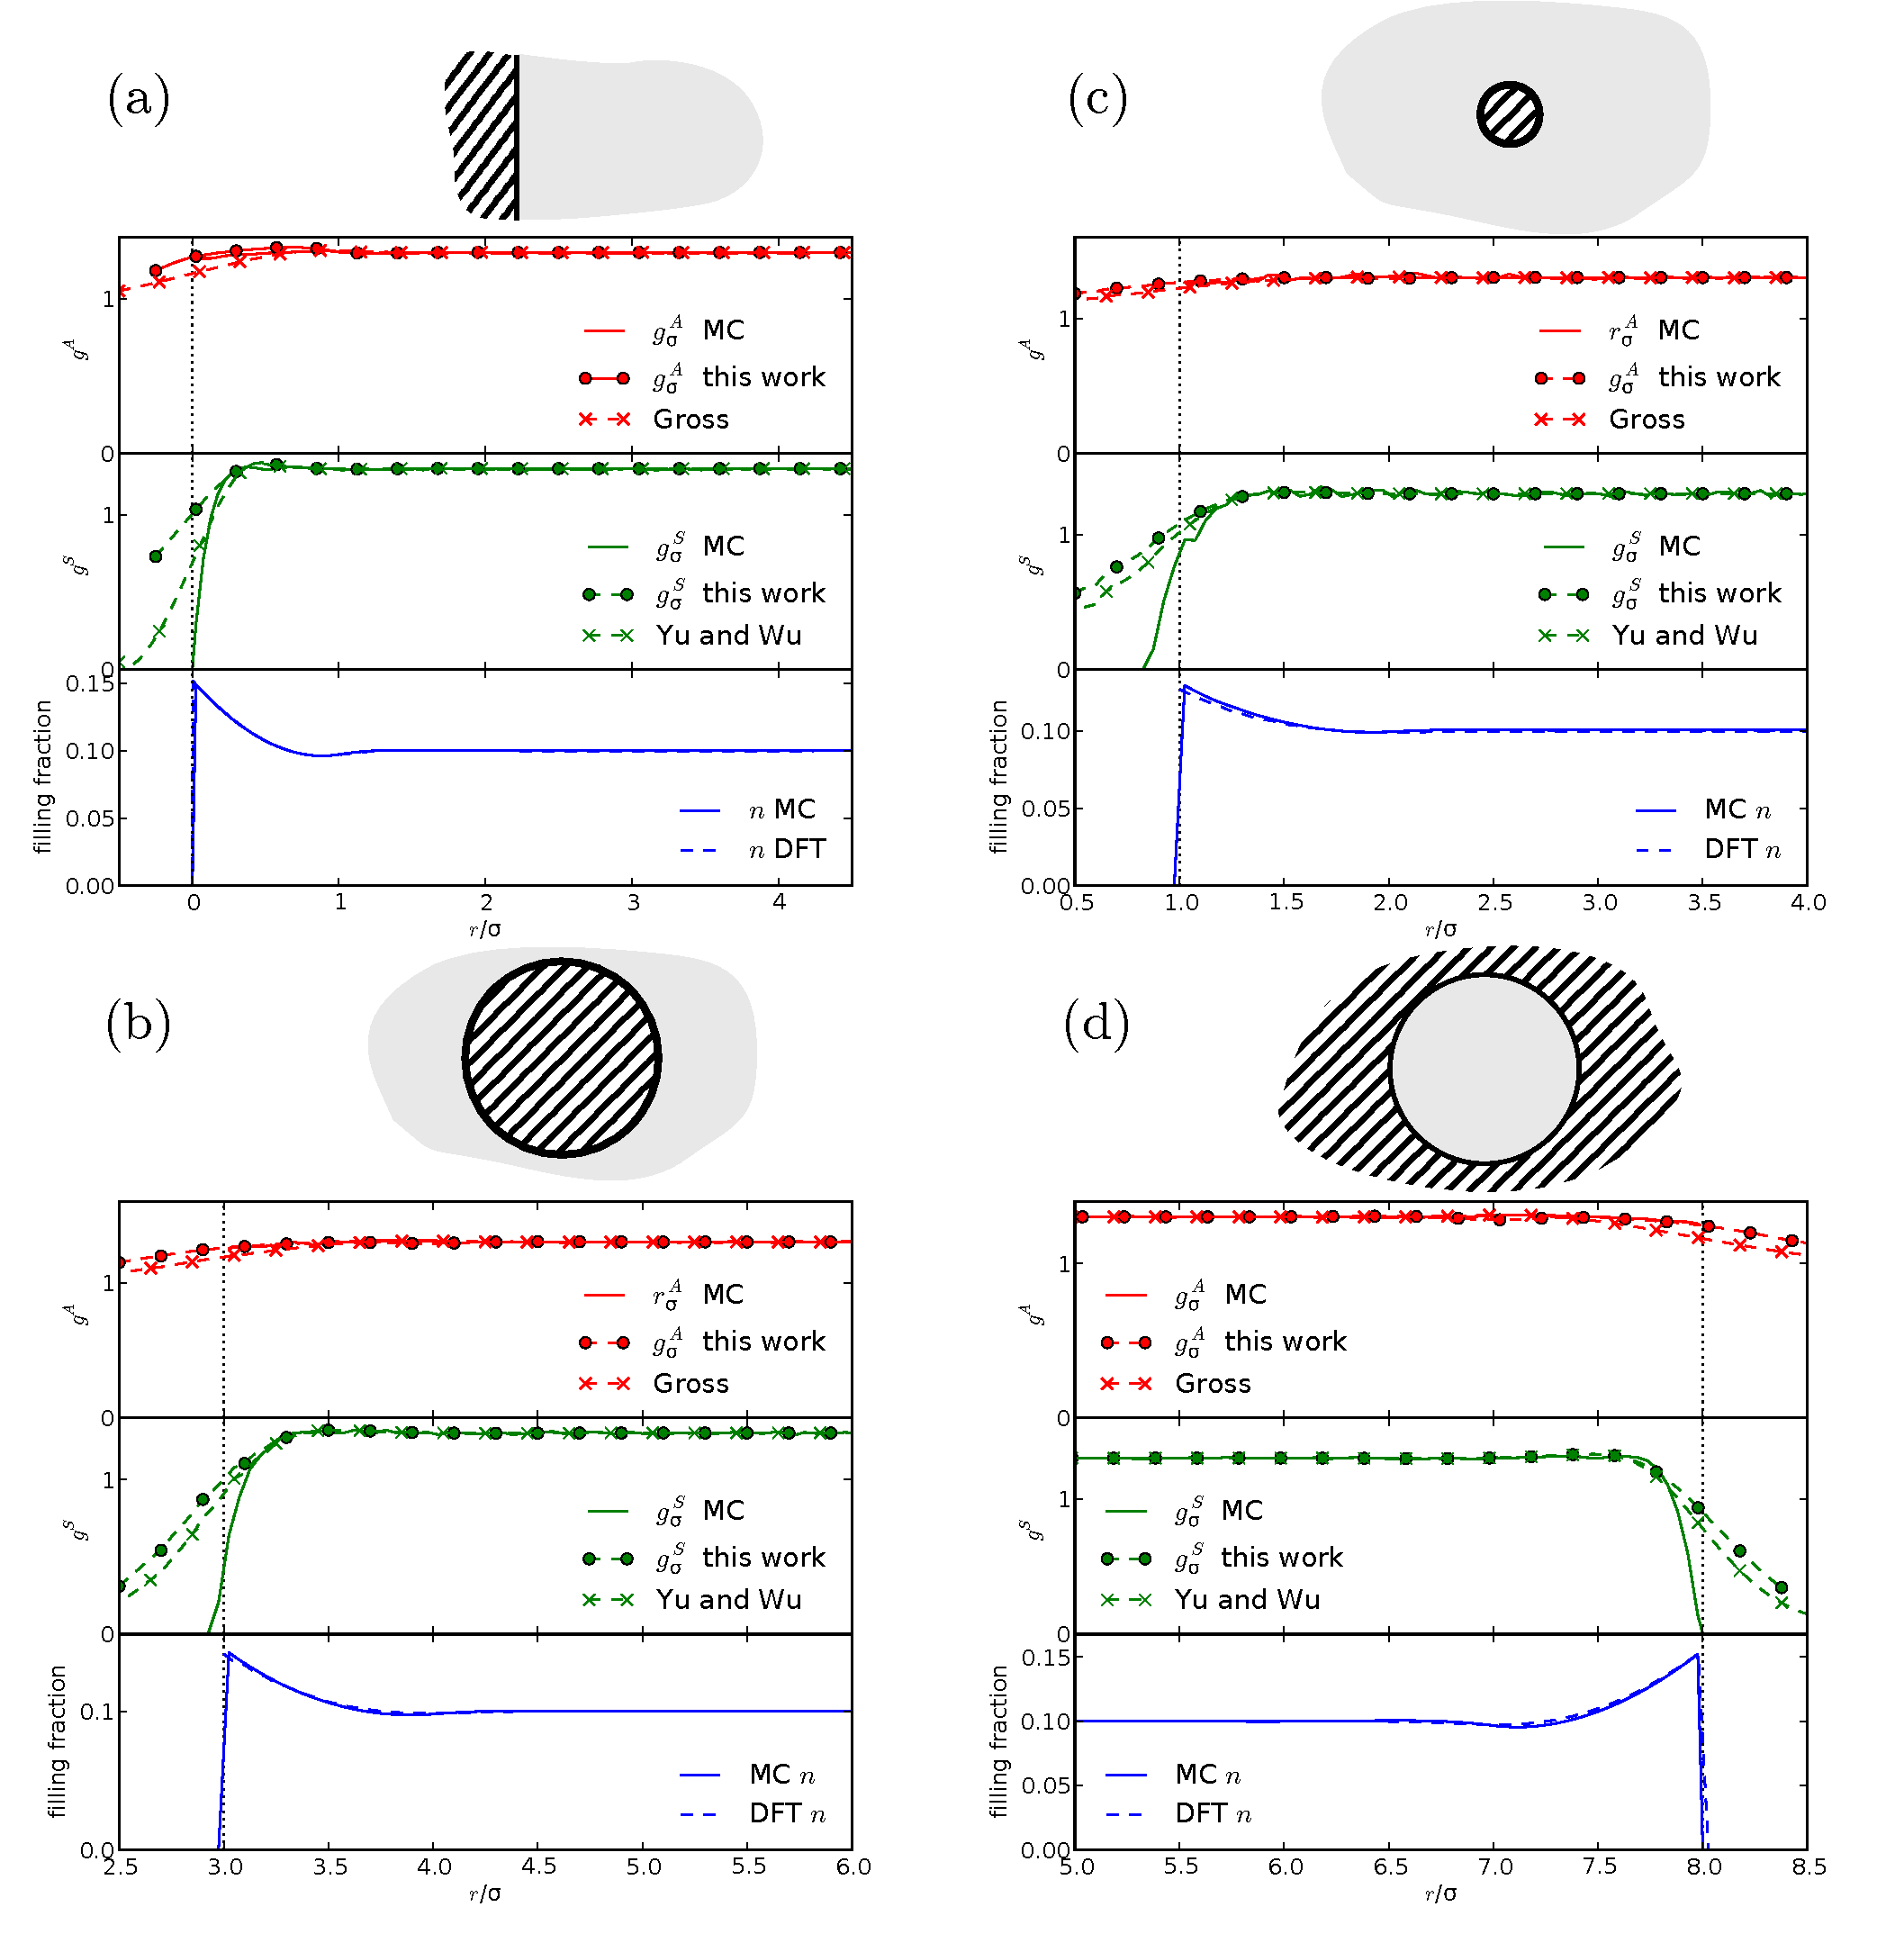
\includegraphics[width=0.8\textwidth]{figs/low-density}
  %% \noindent
  %% \begin{tabular}{cc}
  %%   (a)\includegraphics[width=8cm]{figs/walls-10} &
  %%   (c)\includegraphics[width=8cm]{figs/inner-4-10}\\
  %%   (b)\includegraphics[width=8cm]{figs/inner-12-10} &
  %%   (d)\includegraphics[width=8cm]{figs/outer-16-01}
  %% \end{tabular}
  \caption{ (Color online) Density and distribution function in systems
    with a ``low density'' bulk filling fraction of 0.1.  The
    subplots each show a different system: (a) next to a flat hard wall, (b)
    around a hard sphere with an excluded diameter of $6\sigma$, (c)
    around a hard sphere with an excluded diameter of $2\sigma$, and
    (d) within a spherical cavity with an included diameter of $16\sigma$.
    In the top and middle panels of each subfigure respectively are the
    asymmetrically averaged distribution function $g_\sigma^A$ (defined
    in Equation~\ref{eq:gA}) and the symmetrically averaged
    distribution function $g_\sigma^S$ (defined in
    Equation~\ref{eq:gS}).  The results of Monte Carlo, our
    functional, and one previously published
    functional\cite{gross2009density,
      yu2002fmt-dft-inhomogeneous-associating} are compared in each
    case.  The bottom panels show the density computed with
    Monte Carlo and with DFT.}
  \label{fig:low-density}
\end{figure*}

\subsection{Low density}

We begin by presenting our low-density results, corresponding to a
filling fraction of 0.1, which are shown in
Figure~\ref{fig:low-density}.  At this low density,
the contact value of the distribution function in the bulk is only 1.3,
indicating that correlations are indeed small and that the fluid should be
relatively easy to model.  Indeed, the contact density at the hard
surface is only around 50\% higher than the bulk, and the FMT
predicted density is close to indistinguishable from the true
density for each of the four configurations, as seen in the bottom
subpanel of each subfigure within Figure~\ref{fig:low-density}.

The $g_\sigma^A$ distribution function in each configuration (plotted
in the top panel of each subfigure within
Figure~\ref{fig:low-density}) is very flat, with only small, smooth
changes as the surface is approached.  Our functional $g_\sigma^A$
very closely matches the Monte Carlo predictions in each case, while
that of Gross consistently underestimates the distribution at the
interface by a significant margin.  We note that the theoretical
curves extend into the region from which the fluid is excluded.  This
value corresponds to the distribution function that would be observed
in the vanishingly unlikely scenario in which there was a sphere
present at that location.  Naturally, we am unable to observe this
quantity in our Monte Carlo simulations.

The $g_\sigma^S$ distribution function (plotted
in the middle panels of Figure~\ref{fig:low-density}) shows considerably more
structure, as well as additional variation due to the curvature of the
hard surface.  The symmetric distribution function is nonzero at
locations where spheres may touch, which for a convex hard surface
means that $g_\sigma^S$ may be nonzero in the volume in which hard
spheres are excluded.  In every configuration studied, the agreement
between the theoretical predictions and the Monte Carlo simulation in
each case is very poor in the region where there should be no contacts
at all.  Because $n_0$ is comparable to its bulk value in this region,
this means that these functionals predict a significant number of
contacts in the region where there should be none.  The distribution
function of Yu and Wu~\cite{yu2002fmt-dft-inhomogeneous-associating}
and ours described in Section~\ref{sec:g-S} give similar results, with
slightly larger errors in our prediction.

\begin{figure*}
  \noindent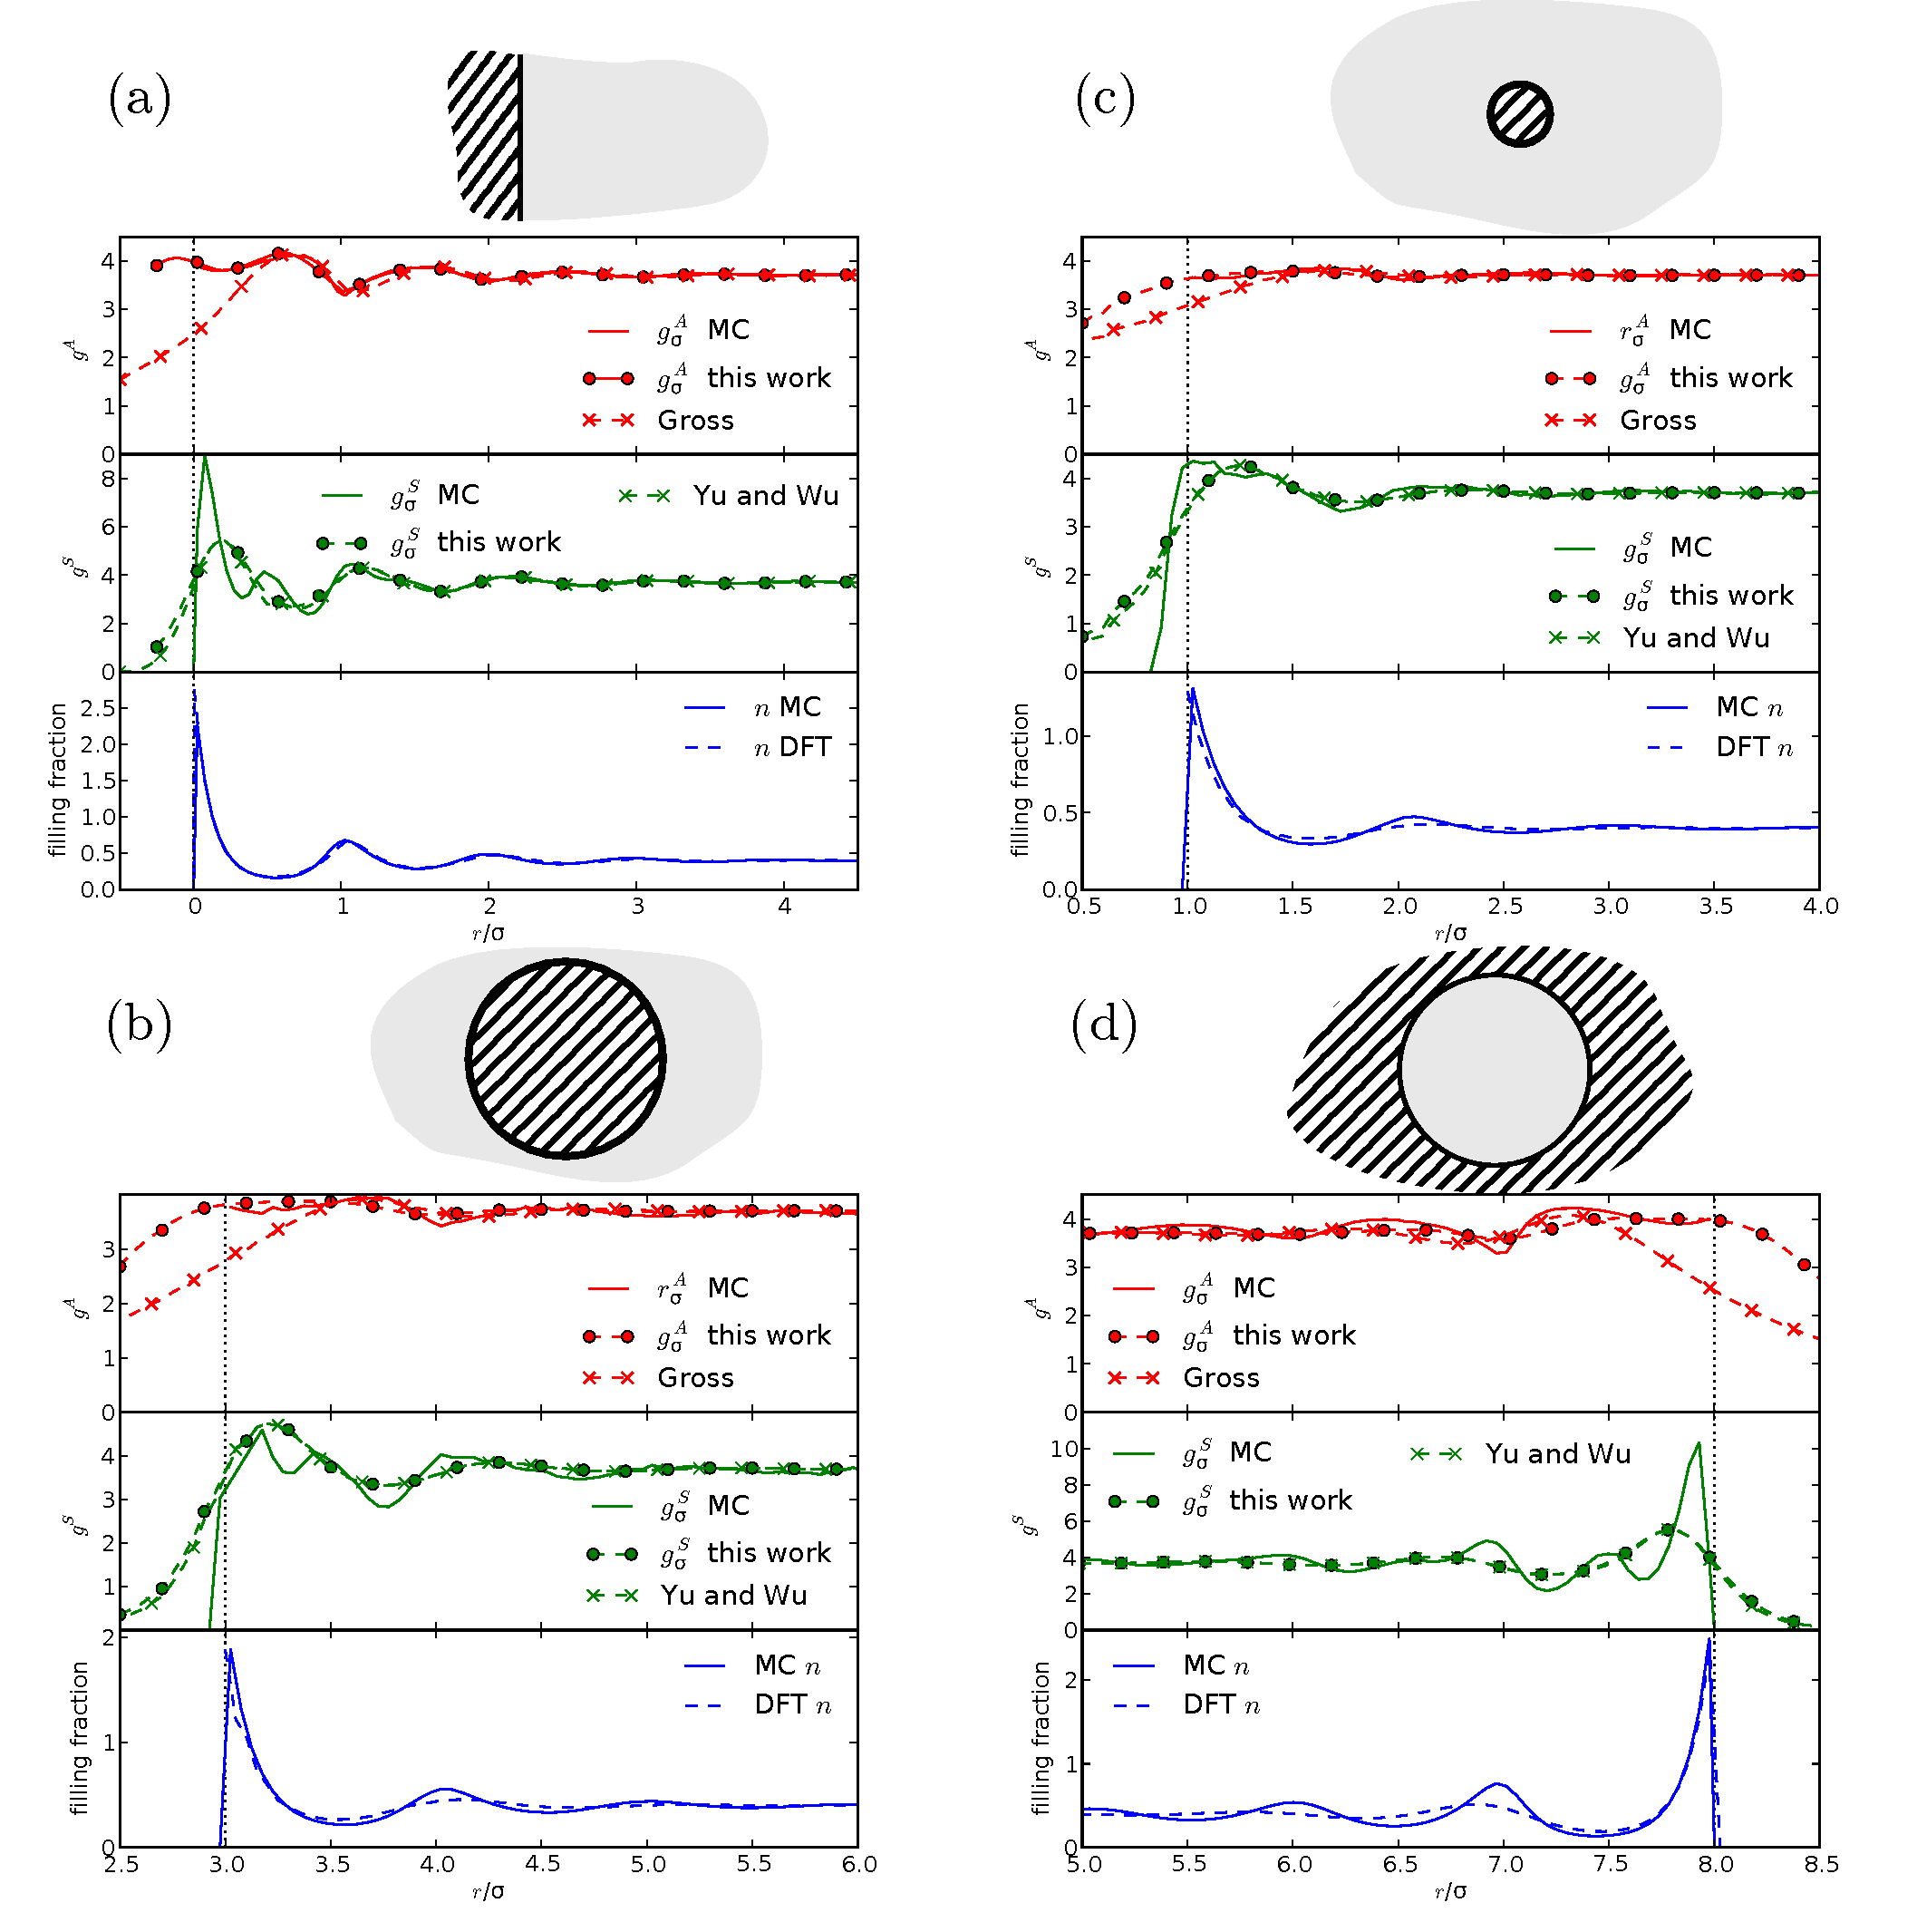
\includegraphics[width=0.8\textwidth]{figs/high-density}
  %% \noindent
  %% \begin{tabular}{cc}
  %%   (a)\includegraphics[width=8cm]{figs/walls-40} &
  %%   (c)\includegraphics[width=8cm]{figs/inner-4-40}\\
  %%   (b)\includegraphics[width=8cm]{figs/inner-12-40} &
  %%   (d)\includegraphics[width=8cm]{figs/outer-16-04}
  %% \end{tabular}
  \caption{ (Color online) Density and distribution function in systems
    with a ``high density'' bulk filling fraction of 0.4.  The
    subplots each show a different system: (a) next to a flat hard wall, (b)
    around a hard sphere with an excluded diameter of $6\sigma$, (c)
    around a hard sphere with an excluded diameter of $2\sigma$, and
    (d) within a spherical cavity with an included diameter of $16\sigma$.
    In the top and middle panels of each subfigure respectively are the
    asymmetrically averaged distribution function $g_\sigma^A$ (defined
    in Equation~\ref{eq:gA}) and the symmetrically averaged
    distribution function $g_\sigma^S$ (defined in
    Equation~\ref{eq:gS}).  The results of Monte Carlo, our
    functional, and one previously published
    functional\cite{gross2009density,
      yu2002fmt-dft-inhomogeneous-associating} are compared in each
    case.  The bottom panels show the density computed with
    Monte Carlo and with DFT.}
  \label{fig:high-density}
\end{figure*}

\subsection{High density}

At a higher density corresponding to a filling fraction of 0.4,
correlations are much stronger, with the bulk contact value of the
distribution function of 3.7, as seen in Figure~\ref{fig:high-density}.
This results in larger oscillations in the density at the hard
surfaces, and correspondingly more interesting behavior in the
distribution function near the interface, as shown in the bottom panels
of the plots in Figure~\ref{fig:high-density}.  The density predicted
by the White Bear functional agrees reasonably well with the
simulation results, although not so well as it did at lower density.
The discrepancies are largest in the case of the spherical cavity
(Figure~\ref{fig:high-density}d), in which the DFT considerably
underestimates the range of the density oscillations.

The asymmetric version of the distribution function (plotted
in the top panels of Figure~\ref{fig:high-density}) once again displays
relatively smooth behavior with a few small
oscillations near the interface, and a somewhat elevated value within
a diameter of the hard surface, with the magnitude of this elevation
somewhat different in each configuration.  As was the case at low
density, our distribution function $g_\sigma^A$ matches very closely
the Monte Carlo data, reproducing quite well the structure near the
interface in each configuration, although in the spherical cavity there is a small, but significant
discrepancy, comparable to the discrepancy found in the density
itself.  In each case, the distribution of Gross dramatically
underestimates the distribution at the interface, at one extreme by
40\% in the case of the spherical cavity
(Figure~\ref{fig:high-density}d), and at the other extreme by 15\%
in the test-particle scenario (Figure~\ref{fig:high-density}c).

%% \begin{figure}
%%   \includegraphics[width=\columnwidth]{figs/outer-16-04}
%%   \caption{Density and distribution functions near the surface of a
%%     spherical cavity with diameter $16\sigma$ at a bulk filling
%%     fraction of 0.4.}
%%   \label{fig:outer-40}
%% \end{figure}

The symmetrically averaged distribution function (plotted
in the middle panels of Figure~\ref{fig:high-density}) shows considerably
more structure near the interface at high density, and this structure
varies considerably depending on the curvature of the hard surface.
In each case, this structure is not reflected in the theoretical
predictions, neither that of this paper, nor that of Yu and
Wu~\cite{yu2002fmt-dft-inhomogeneous-associating}.  As was the case at
low density, both functionals give significant and finite values in
the region in which there are no contacts, but at high density they
also miss the large oscillations that are present near the flat wall
and the concave surface (Figures~\ref{fig:high-density}a
and~\ref{fig:high-density}d).  As was the case at low density, the
functional of Yu and Wu~\cite{yu2002fmt-dft-inhomogeneous-associating}
gives slightly better agreement with the simulation results than that
which we derive in Section~\ref{sec:g-S}.

%%%%%%%%%%%%%%%%%%%%%%%%%%%%%%%%%%%%%%%%%%%%%%%%%%%%%%%%%%%%
\section{Conclusion}
We investigated several approximations to the contact value of the
distribution function for inhomogeneous fluid distributions
corresponding to flat, concave, and convex walls.  We
defined and simulated two averages of the distribution function, an
asymmetric $A$ average centered at the location of one of the two
spheres that is in contact, and a symmetric $S$ average centered at
the point of contact of touching spheres.  For each average, we
derived a functional form from FMT, and also found an approximation
that has been used in the literature.  When compared with essentially
exact Monte Carlo simulations, the $A$ distribution function derived
from Fundamental Measure Theory in Section~\ref{sec:g-A} gives
excellent results for each surface, at both high density and low
density.  The other three approximations that we studied all showed
significant and systematic deviations under some circumstances.  Thus,
we recommend that creators of SAFT-based classical density functionals
consider using the $g_\sigma^A$ functional defined in
Section~\ref{sec:g-A}.



%% \begin{figure}
%% \includegraphics[width=\columnwidth]{figs/gHS-vs-n}
%% \caption{A comparison of the various approximations to the contact
%%   density in the homogeneous limit.  As expected, they are all
%%   identical, and we won't include this plot in the paper (but it's
%%   here to verify that our code is working).}
%% \label{fig:gHS-vs-n}
%% \end{figure}

%% \begin{figure}
%% \includegraphics[width=\columnwidth]{figs/free-energy}
%% \caption{A comparison of the various approximations to the free energy
%%   in the homogeneous limit.  Note that the White Bear functional uses
%%   a modified form of the Carnahan equation of state.  As expected,
%%   these are all identical, and we won't include this plot in the paper
%%   (but it's here to verify that our code is working).}
%% \label{fig:free-energy}
%% \end{figure}

$\mathbf{Appendix~to~Chapter~\ref{chapter:contact}}$

The expression for the asymmetric distribution function
$g_\sigma^A(\rr)$ (Equation~\ref{eq:g-A-exact}) involves the
functional derivative $\frac{\delta F_{HS}}{\delta
  \sigma(\mathbf{r})}$.  In this appendix we will explain how this
derivative is evaluated.  We begin by applying the chain rule in the
following way:
  \begin{align}
    \frac{\delta F_{HS}}{\delta \sigma(\mathbf{r})} &=
    \int \left(
    \sum_\alpha
    \frac{\delta F_{HS}}{\delta n_\alpha(\mathbf{r}')}
    \frac{\delta n_\alpha(\mathbf{r}')}{\delta \sigma(\mathbf{r})}
    \right) d\mathbf{r}'
  \end{align}
This expression requires us to evaluate $\frac{\delta F_{HS}}{\delta
  n_\alpha(\mathbf{r}')}$ and $\frac{\delta
  n_\alpha(\mathbf{r}')}{\delta \sigma(\mathbf{r})}$.  The former is
straightforward, given Equations~\ref{eq:Phi1}-\ref{eq:Phi3}, and we
will write no more about it.  The functional derivatives of the
fundamental measures, however, require a bit more subtlety, and we
will address them here.

We begin with the derivative of $n_3$, the filling fraction, which we
will discuss in somewhat more detail than the remainder, which are
similar in nature.  Because the diameter $\sigma(\rr)$ is the diameter
of a sphere \emph{at position~$\rr$}, we write the fundamental measure
$n_3(\rr')$ as
\begin{align}
  n_3(\rr') &= \int n(\rr'') \Theta\left(\frac{\sigma(\rr'')}{2}
  -\left|\rr' - \rr''\right|\right)
  d\rr''
\end{align}
where we note that $\sigma(\rr'')$ and $n(\rr'')$ are the diameter and
density, respectively, of spheres centered at position~$\rr''$.  Thus the
derivative with respect to the diameter of spheres at position
$\rr$ is
\begin{align}
  \frac{\delta n_3(\rr')}{\delta \sigma(\rr)} &= \frac 12 \int n
  (\rr'') \delta\left(\frac{\sigma(\rr'')}{2} -\left|\rr' - \rr''\right|\right)
  \delta(\rr-\rr'') d\rr'' \\ &= n (\rr) \delta(\sigma(\rr)/2
  -\left|\rr' - \rr\right|)
\end{align}
This pattern will hold for each fundamental measure: because we are
seeking the change in free energy when spheres at point~$\rr$ are
expanded, the integral over density is eliminated.  To compute the
distribution funtion $g_\sigma^A$, we convolve this delta function with
the product of the density and a local derivative of $\Phi(\rr)$:
\begin{align}
  \frac{\delta F_{HS}}{\delta \sigma(\rr)} &= \int \frac{\partial \Phi(\rr')}{\partial
    n_3(\rr')}n(\rr') \delta(\sigma/2-|\rr'-\rr|)d\rr'
  + \cdots
\end{align}
As we shall see, there are only four convolution kernels, leading to
four additional convolutions beyond those required for FMT.

The functional derivative of $n_2$ introduces our second convolution
kernel, which is a derivative of the delta function.
\begin{align}
  %n_2(\rr') &= \int n(\rr'') \delta(\sigma(\rr'')/2 -\left|\rr' - \rr''\right|) d \rr''\\
  \frac{\delta n_2(\rr')}{\delta \sigma(\rr)} &= \frac 12 n(\rr) \delta'(\sigma(\rr)/2 -\left|\rr' - \rr\right|)
\end{align}
The derivatives of the remaining scalar densities $n_1$ and $n_0$ reduce to
sums of the terms above:
\begin{align}
  %n_1(\rr') &= \int \mathbf{dr''} \frac{n(\rr'')}{2\pi \sigma(\rr'')}
  %\delta(\sigma(\rr'')/2 -\left|\rr' - \rr''\right|) \\
  \frac{\delta n_1(\rr')}{\delta \sigma(\rr)}
  = \frac{n(\rr)}{4\pi
    \sigma(\rr)}\delta'(\sigma(\rr)/2 -\left|\rr' - \rr\right|) 
  -
  \frac{n(\rr)}{2\pi
    \sigma(\rr)^2}\delta(\sigma(\rr)/2 -\left|\rr' - \rr\right|)
\end{align}
and
\begin{align}
  %n_0(\rr') &= \int \mathbf{dr''} \frac{n(\rr'')}{\pi \sigma(\rr'')^2}
  %\delta(\sigma(\rr'')/2 -\left|\rr' - \rr''\right|) \\
  \frac{\delta n_0(\rr')}{\delta \sigma(\rr)}
  = \frac{n(\rr)}{2\pi
    \sigma(\rr)^2}\delta'(\sigma(\rr)/2 -\left|\rr' - \rr\right|)
  -
  2 \frac{n(\rr)}{\pi
    \sigma(\rr)^3}\delta(\sigma(\rr)/2 -\left|\rr' - \rr\right|)
\end{align}

The vector-weighted densities $\mathbf{n}_{V1}$ and $\mathbf{n}_{V2}$
give terms analogous to those of $n_1$ and $n_2$:
\begin{align}
  %\mathbf{n}_{V2}(\rr') &= \int n(\rr') \delta(\sigma(\rr'')/2 -\left|\rr' - \rr''\right|)
  %  \frac{\rr'-\rr''}{|\rr'-\rr''|} d \rr''\\
  \frac{\delta \mathbf{n}_{V2}(\rr')}{\delta \sigma(\rr)} = -\frac 12 n(\rr) \delta'(\sigma(\rr)/2 -\left|\rr' - \rr\right|)
    \frac{\rr-\rr'}{|\rr-\rr'|}
\end{align}
\begin{align}
  %\mathbf{n}_{V1}(\rr') &= \int d\rr'' \frac{n(\rr'')}{2\pi \sigma(\rr'')}
  %\delta(\sigma(\rr'')/2 -\left|\rr' - \rr''\right|) \frac{\rr'-\rr''}{|\rr'-\rr''|}\\
  \frac{\delta \mathbf{n}_{V1}(\rr')}{\delta \sigma(\rr)}
  = -\frac{n(\rr)}{4\pi
    \sigma(\rr)}\delta'(\sigma(\rr)/2 -\left|\rr' - \rr\right|) \frac{\rr-\rr'}{|\rr-\rr'|}
  \\ +
  \frac{n(\rr)}{2\pi
    \sigma(\rr)^2}\delta(\sigma(\rr)/2 -\left|\rr' - \rr\right|) \frac{\rr-\rr'}{|\rr-\rr'|}
\end{align}
Thus there are four convolution kernels used in computing $g_\sigma^A$:
one scalar and one vector delta function, and one scalar and one
vector derivative of the delta function.

\clearpage
\newpage
\chapter{Improved Association Term in SAFT DFT for water}
\def\re{\text{Re}}
\def\im{\text{Im}}
\def\ket#1{\vert #1 \rangle}
\def\cU{{\cal{U}}}
\def\cD{{\cal{D}}}
\def\re{\text{Re}}
\def\im{\text{Im}}
%\newcommand{\red}[1]{{\bf \color{red} #1}}
%\newcommand{\blue}[1]{{\bf \color{blue} #1}}
%\newcommand{\green}[1]{{\bf \color{green} #1}}
%\newcommand{\rr}{\textbf{r}}
%\newcommand{\xx}{\textbf{r}}
%\newcommand{\refnote}{\red{[ref]}}

\newcommand\etadisp{\ensuremath{\eta_\textit{d}}}
\newcommand\epsilondisp{\ensuremath{\epsilon_\textit{d}}}
\newcommand\epsilonassoc{\ensuremath{\epsilon_\textit{a}}}
\newcommand\kappaassoc{\ensuremath{\kappa_\textit{a}}}
\newcommand\lambdadisp{\ensuremath{\lambda_\textit{d}}}
\newcommand\lscale{\ensuremath{s_d}}

% fixme is intended to prioritize stuff that needs fixing.
%\newcommand{\fixme}[1]{\textcolor{red}{[\emph{#1}]}}
%\newcommand\hughesetal{Ref.~\citenum{hughes2013classical}}
\newcommand\hughesetal{Hughes \emph{et al.}}

\newcommand\hughesetalcite{Hughes \emph{et al.}~\cite{hughes2013classical}}

%%%%%%%%%%%%%%%%%%%%%%%%%%%%%%%%%%%%%%%%%%%%%%%%%%%%%%%%%%%%
\section{Introduction}
In this chapter we present a modification to our recently published
SAFT-based classical density functional theory for water.
%
We have recently developed and tested a functional for the averaged
radial distribution function at contact of the hard-sphere fluid
that is dramatically more accurate at interfaces than earlier
approximations.
%
We now incorporate this improved functional into the association term
of our free energy functional for water, improving its description of
hydrogen bonding.
%
We examine the effect of this improvement by studying two hard solutes
(a
hard hydrophobic rod and a hard sphere) and a Lennard-Jones
approximation of a krypton atom solute.
%
The improved functional leads to a moderate change in the density
profile and a large decrease in the number of hydrogen bonds broken in
the vicinity of the hard solutes.
%
We find an improvement of the partial radial distribution for a
krypton atom in water when compared with experiment.


Water, the universal solvent, is of critical practical importance, and
a continuum description of water is in high demand for a solvation
model.  A number of recent attempts to develop improved solvation
models for water have built on the approach of classical
density functional theory (DFT)~\cite{jeanmairet2013molecular,
  zhao2011molecular, zhao2011new, ramirez2005direct,
  ramirez2005density, levesque2012solvation, levesque2012scalar}.
There are two general
approaches used to construct a classical DFT for water.  The first is
to choose a convenient functional form which is then fit to properties
of the bulk liquid at a given temperature and pressure
\cite{jeanmairet2013molecular, zhao2011molecular, zhao2011new,
  ramirez2005direct, ramirez2005density, levesque2012solvation,
  levesque2012scalar, lischner2010classical}.  Using this approach, it
is possible to construct a functional that reproduces the exact
second-order response function of the liquid under the fitted
conditions.  However, this class of functional will be less accurate
at other temperatures or pressures---and in the inhomogeneous
scenarios in which solvation models are applied.  The second approach
is to construct a functional by applying liquid-state theory to a
model system, and then fit the model to experimental data such as the
equation of state~\cite{hughes2013classical, clark2006developing,
  gloor2002saft, gloor2004accurate, gloor2007prediction, Jaqaman2004,
  chuev2006, fu2005vapor-liquid-dft,kiselev2006new,
  blas2001examination, sundararaman2012computationally}.
%%  Classical
%% DFT is a natural framework for creating a more flexible theory of
%% hydrophobicity that can readily describe interaction of water with
%% arbitrary external potentials---such as potentials describing strong
%% interactions with solutes or surfaces.

The association contribution to the SAFT free energy uses
Wertheim's first-order thermodynamic perturbation theory to describe
an associating fluid as hard-spheres with strong associative
interactions at specific sites on the surface of each
sphere~\cite{wertheim1984fluidsI, wertheim1984fluidsII,
  wertheim1986fluidsIII, wertheim1986fluidsIV}.  These association
sites have an attractive interaction at contact, and rely on the
hard-sphere pair distribution function at contact $g_\sigma^\text{HS}$
in order to determine the extent of association.  While this function
is known for the homogeneous hard-sphere fluid, it must be
approximated for inhomogeneous systems, such as occur at liquid
interfaces.

In Chapter~\ref{chapter:contact} we examined the pair distribution
function at contact in various inhomogeneous
configurations~\cite{schulte2012using}.  We tested the accuracy of
existing approximations for the pair distribution function at
contact~\cite{yu2002fmt-dft-inhomogeneous-associating,
gross2009density}, and derived a significantly improved approximation
for the averaged distribution function at contact.  In this chapter we
apply this improved $g_\sigma^{HS}$ to the SAFT-based classical
density functional for water developed by Hughes \emph{et
al.}~\cite{hughes2013classical}.  This functional was constructed to
reduce in the homogeneous limit to the 4-site optimal SAFT model for
water developed by Clark \emph{et al.}~\cite{clark2006developing}.
The DFT of \hughesetal\ uses the association free energy functional of
Yu and Wu~\cite{yu2002fmt-dft-inhomogeneous-associating}, which is
based on a $g_\sigma^{HS}$ that we have since found to be
inaccurate~\cite{schulte2012using}.  In this chapter, we will examine
the result of using the improved functional for $g_\sigma^{HS}$ to
construct an association free energy functional.

\section{Method}

The classical density functional for water of \hughesetal\ consists of
four terms:
\begin{align}
  F[n(\rr)] &= F_{\text{ideal}}[n(\rr)] + F_{\text{HS}}[n(\rr)]
  + F_{\text{disp}}[n(\rr)] + F_{\text{assoc}}[n(\rr)]
\end{align}
where $F_{\text{ideal}}$ is the ideal gas free energy and
$F_{\text{HS}}$ is the hard-sphere excess free energy, for which we
use the White Bear functional~\cite{roth2002whitebear}.
$F_{\text{disp}}$ is the free energy contribution due to the
square-well dispersion interaction; this term contains one empirical
parameter, $\lscale$, which is used to fit the surface tension of water near one
atmosphere.  Finally, $F_{\text{assoc}}$ is the free energy
contribution due to association, which is the term that we examine in
this chapter.

\subsection{Dispersion}
The dispersion term in the free energy includes the van
der Waals attraction and any orientation-independent
interactions. Following \hughesetal, we use a dispersion term based on
the SAFT-VR approach\cite{gil-villegas-1997-SAFT-VR}, which has two
free parameters (taken from Clark~\emph{et
  al}\cite{clark2006developing}): an interaction energy $\epsilondisp$
and a length scale $\lambdadisp R$.

The SAFT-VR dispersion free energy has the form~\cite{gil-villegas-1997-SAFT-VR}
\begin{align}
  F_\text{disp}[n] &= \int \left(a_1(\xx) + \beta a_2(\xx)\right)n(\xx)d\xx
  \label{eq:dispersion-term}
\end{align}
where $a_1$ and $a_2$ are the first two terms in a high-temperature
perturbation expansion and $\beta=1/k_BT$.  The first term, $a_1$, is
the mean-field dispersion interaction. The second term, $a_2$, describes the
effect of fluctuations resulting from compression of the fluid due
to the dispersion interaction itself, and is approximated
using the local compressibility approximation (LCA), which
assumes the energy fluctuation is simply related to the
compressibility of a hard-sphere reference fluid\cite{barker1976liquid}.

The form of $a_1$ and $a_2$ for SAFT-VR is given in
reference~\cite{gil-villegas-1997-SAFT-VR}, expressed in terms
of the packing fraction.  In order to apply this form to an
\emph{inhomogeneous} density distribution, we construct an effective local
packing fraction for dispersion $\etadisp$, given by a Gaussian
convolution of the density:
\begin{align}
  \etadisp(\xx) &= \frac{1}{6\sqrt{\pi} \lambdadisp^3\lscale^3}
  \int n(\xx')\exp\left({-\frac{|\xx-\xx'|^2}{2(2 \lambdadisp
      \lscale R)^2}}\right)d\xx'.\label{eq:packing-fraction}
\end{align}
This effective packing fraction is used throughout the dispersion
functional, and represents a packing fraction averaged over the
effective range of the dispersive interaction.
Eq.~\ref{eq:packing-fraction} contains an additional empirical
parameter $\lscale$ introduced by \hughesetal, which modifies the
length scale over which the dispersion interaction is correlated.

\begin{figure}
\begin{center}
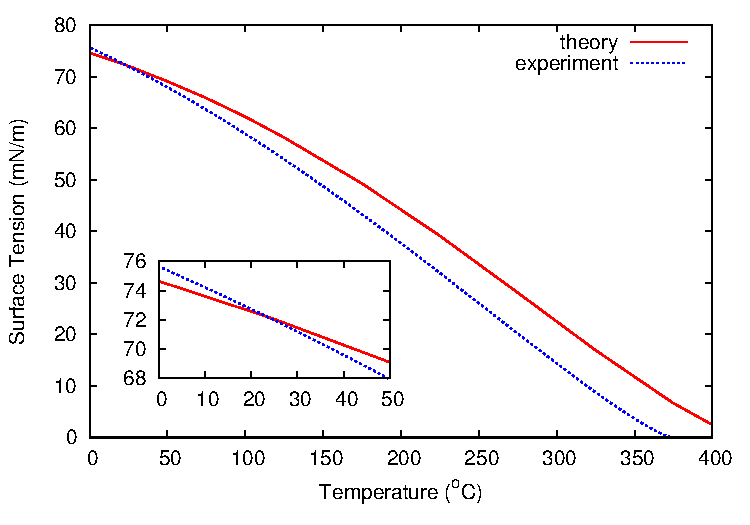
\includegraphics[width=3.5in]{figs/surface-tension}
\end{center}
\caption{Comparison of Surface tension versus temperature for
  theoretical and experimental data. The experimental data is taken
  from NIST~\cite{nistwater}.  The length-scaling parameter $\lscale$
  is fit so that the theoretical surface tension will match the
  experimental surface tension near room temperature.}
\label{fig:surface-tension}
\end{figure}

\subsection{Association}

The association free energy for our four-site model has the form:
\begin{align}
  F_\text{assoc}[n] &= k_BT \int n_\text{site}(\xx)
  \left(\ln X(\xx) - \frac{X(\xx)}{2} + \frac12\right) d\xx
\end{align}
where $n_\text{site}(\rr)$ is the density of bonding sites at
position~$\rr$:
\begin{align}
  n_\text{site}(\rr) &=
  \begin{cases}
    4 n(\rr) & \text{this work}\\
    4 n_0(\rr) \zeta(\rr) & \text{\hughesetalcite}
  \end{cases}
\end{align}
where the factor of four comes from the four hydrogen bond sites, the
fundamental measure $n_0(\rr)$ is the average density contacting point
$\rr$, and $\zeta(\xx)$ is a dimensionless measure of the density
inhomogeneity from Yu and
Wu~\cite{yu2002fmt-dft-inhomogeneous-associating}.  The functional
$X(\rr)$ is the fraction of association sites \emph{not}
hydrogen-bonded, which is determined for our 4-site model by the
quadratic equation
\begin{align}
  X(\xx) &= \frac{\sqrt{1 + 2n_\text{site}'(\rr)
      \kappaassoc g^\textit{SW}_\sigma(\xx)
  \left(e^{\beta\epsilonassoc} - 1\right)} - 1}
  {n_\text{site}'(\rr)
    \kappaassoc g^\textit{SW}_\sigma(\xx)
  \left(e^{\beta\epsilonassoc} - 1\right)}, \label{eq:X}
\end{align}
where
\begin{align}
  n_\text{site}'(\rr) &=
  \begin{cases}
    \frac{4}{\pi\sigma^2} \int n(\rr')\delta(\sigma - |\rr-\rr'|) d\rr' & \text{this work}\\
    4 n_0(\rr) \zeta(\rr) & \text{\hughesetal}
  \end{cases}
\end{align}
is the density of bonding sites that could bond to the sites~$n_\text{site}(\rr)$, and
\begin{align}
  g^\textit{SW}_\sigma(\xx) &= g^\textit{HS}_\sigma(\xx) +
  \frac{1}{4}\beta\left(\frac{\partial a_1}{\partial \etadisp(\xx)} -
  \frac{\lambdadisp}{3 \etadisp}\frac{\partial a_1}{\partial \lambdadisp}\right)\label{eq:gSW},
\end{align}
%This is equation 77 of gil-villegas-1997-SAFT-VR
where $g^\textit{HS}_\sigma$ is the correlation function evaluated at
contact for a hard-sphere fluid with a square-well dispersion
potential, and $a_1$ and $a_2$ are the two terms in the dispersion
free energy defined below Eq.~\ref{eq:dispersion-term}.  The radial distribution function of the square-well
fluid $g^\textit{SW}_\sigma$ is written as a perturbative correction
to the hard-sphere radial distribution function
$g^\textit{HS}_\sigma$.  The functional of \hughesetal\ uses the
$g_\sigma^\textit{HS}$ from Yu and Wu
\cite{yu2002fmt-dft-inhomogeneous-associating}.  In this work, we use
the $g_\sigma^\textit{HS}$ derived by Schulte~\emph{et~al.}~\cite{schulte2012using}.

As in \hughesetal, we use Clark's five empirical parameters, and fit
the calculated surface tension to experimental surface tension at
ambient conditions by tuning the parameter $\lscale$, which adjusts
the length-scale of the average density used for the dispersion
interaction.  With the improved association term, we find these agree
when $\lscale$ is 0.454, which is an increase from the value of 0.353
found by \hughesetal.  In order to explore further the change made by
the improved association term, we compared the new functional with
that of \hughesetal\ for the two hydrophobic cases of the hard rod and
the hard spherical solute.

\begin{figure}
\begin{center}
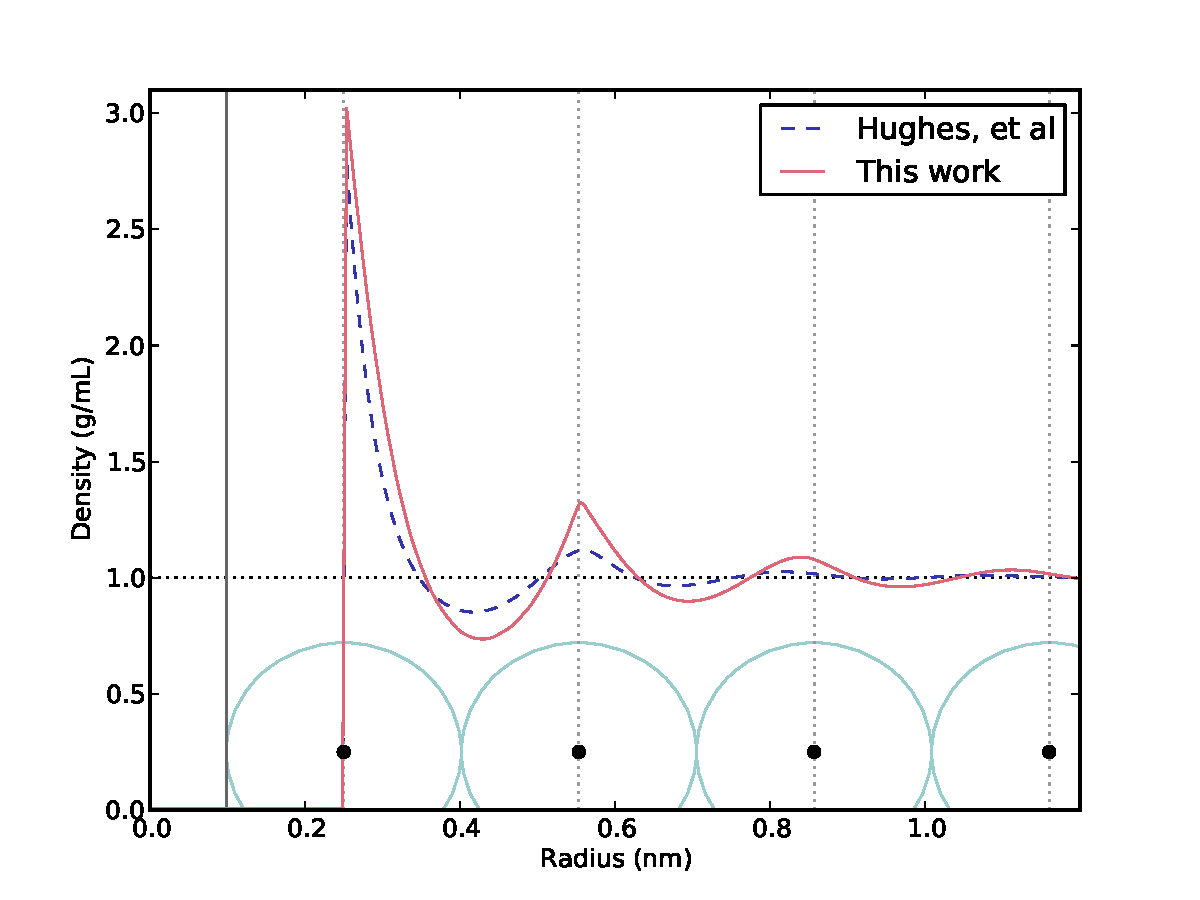
\includegraphics[width=3.5in]{figs/density-compare}
\end{center}
\caption{ Density profiles for a water around a single hard rod
  of radius 0.1~nm. The solid red profile is from the functional
  developed in this chapter and the dashed blue profile is the result
  from \hughesetal.  For scale, under the profiles
  is a cartoon of a string of hard spheres touching in one
  dimension. The horizontal black dotted line is the bulk density for
  water and the vertical line on the left at 0.1~nm represents the
  rod wall.}
\label{fig:density-single-rod}
\end{figure}

\section{Results}

We will first discuss the case of a single hard rod immersed in
water. Figure~\ref{fig:density-single-rod} shows the density profile
of water near a rod with radius~1~\AA.  The density computed using the
functional of this chapter is qualitatively similar to that from
\hughesetal, with a comparable density at contact---consistent with
having made only a moderate change in the free energy.  The first
density peak near the surface is higher than that from \hughesetal,
and the peak has a kink at the top.  This reflects the improved
accuracy of the $g_\sigma^\textit{HS}$ from \hughesetal, since beyond
the first peak water molecules are unable to touch---or hydrogen bond
to---molecules at the surface of the hard rod. This is illustrated
under the profiles in Figure~\ref{fig:density-single-rod} by a cartoon
of adjacent hard spheres that are increasingly distant from the hard
rod surface.

\begin{figure}
\begin{center}
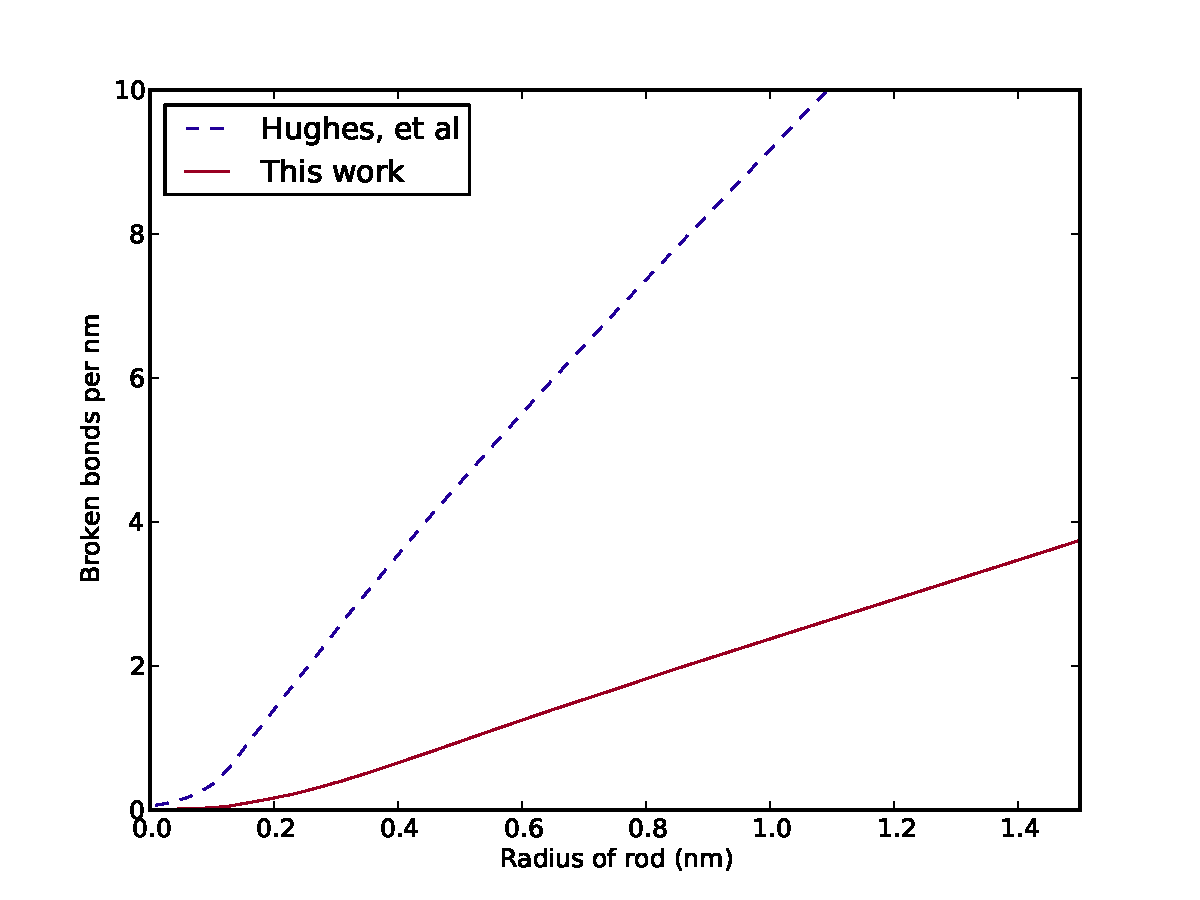
\includegraphics[width=3.5in]{figs/single-rod-broken-HB}
\end{center}
\caption{Broken hydrogen bonds per nanometer for hard rods
  immeresed in water.  The solid red line uses the functional developed
  in this chapter while the dashed blue line uses the functional from
  \hughesetal. For large enough rods, the graph
  increases linearly for both functionals.}
\label{fig:single-rod-broken-HB}
\end{figure}

In addition to the density, we examine the number of hydrogen bonds
which are broken due to the presence of a hard rod.  We define this
quantity as
\begin{align}
  N_{\text{broken HB}} &= 2 \int (X(\rr) - X_{\text{bulk}})n_{\text{site}}(\rr) d\rr
\end{align}
where $X_{\text{bulk}} = 0.13$ is the fraction of unbonded
association sites in the bulk.  The factor of 2 is chosen to account
for the four association sites per molecule, and the fact that each
broken hydrogen bond must be represented twice---once for each of the
molecules involved.  In Fig.~\ref{fig:single-rod-broken-HB} we show
the number of hydrogen bonds broken by a hard rod per nanometer
length, as predicted by the functional of \hughesetal\ (dashed line)
and this work (solid line), as a function of the radius of the hard
rod.  In each case in the limit of large rods, the number of broken
bonds is proportional to the surface area.  At every radius, the
functional of \hughesetal\ predicts approximately four times as many
broken hydrogen bonds as the improved functional.

A common test case for studying hydrophobic solutes in water is the
hard-sphere solute.  Figure~\ref{fig:spheres-broken-HB} shows results
for the number of broken hydrogen bonds caused by a hard-sphere solute,
as a function of the solute radius.  As in
Fig.~\ref{fig:single-rod-broken-HB}, the number of broken bonds scales
with surface area for large solutes, and the number of broken bonds is
about four times smaller than the number from the functional of
\hughesetal.  For solutes smaller than
3~\AA\ in radius, there is less than a tenth of a hydrogen bond
broken. This is consistent with the well-known fact that small solutes
(unlike large solutes) do not disrupt the hydrogen-bonding network of
water~\cite{chandler2005}.

\begin{figure}
\begin{center}
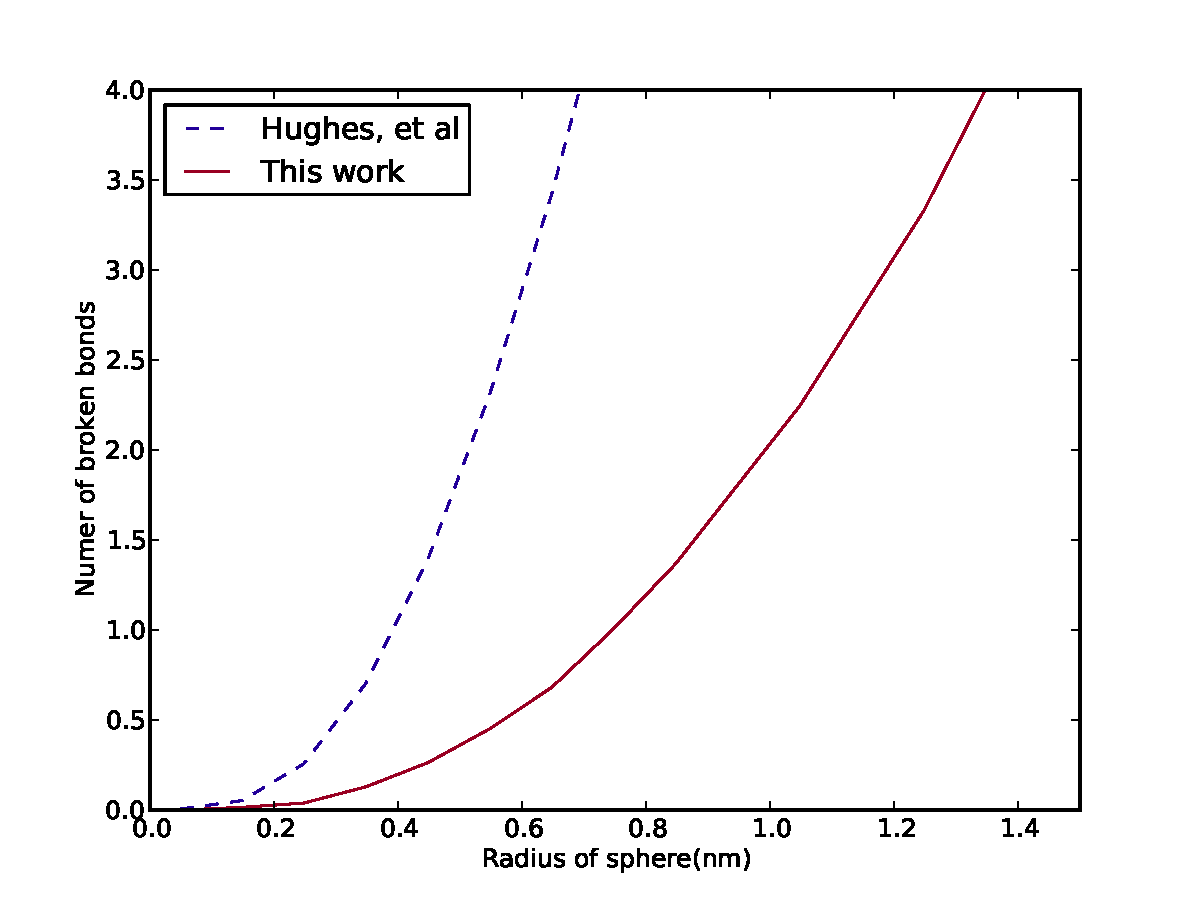
\includegraphics[width=3.5in]{figs/sphere-broken-HB}
\end{center}
\caption{Broken hydrogen bonds for hard spheres immeresed in water.
  The solid red line uses our the functional developd in this chapter
  while the dashed blue line is from
  \hughesetal.}
\label{fig:spheres-broken-HB}
\end{figure}

Finally, in order to compare with experimental results, we examined
the hydration of Krypton.  To describe the interaction of water with
krypton, we use a Lennard-Jones potential with values $\epsilon =
.9518$~kJ/mol and $\sigma = 3.42$~\AA\ calculated using the
Lorentz-Berthelot mixing rules and the Lennard-Jones parameters for
water from SPC/E
calculations~\cite{paschek2004temperature}. Figure~\ref{fig:g-Kr}
shows the krypton-oxygen partial radial distribution function
$g_{Kr-O}(r)$, which gives the relative probability density that an
oxygen atom resides at a distance $r$ from a krypton atom centered at
the origin.  We present theoretical curves computed using both this
work and the functional of \hughesetal, which we compare with
experimental data from extended x-ray absorption fine structure
spectroscopy~(EXAFS)~\cite{bowron1998hydrophobic}.  The new functional
shows improved agreement with experiment in the height and position
of the first maximum as well as the hight and position of the first
minimum in $g_{Kr-O}(r)$ when compared with that of \hughesetal \

%% \section{New stuff}

%% \begin{figure}
%%   \begin{center}
%%     \includegraphics[width=3.5in]{figs/lj-Xe-energy}
%%   \end{center}
%%   \caption{Here is xenon.}
%%   \label{fig:xe-energy}
%% \end{figure}

%% Excess free energy for single Lennard-Jones atoms in water \fixme{are
%%   shown} and compared with simulation of other water theories
%% \cite{paschek2004temperature}and experiment in \fixme{a figure}.

%% \begin{center}
%%   \begin{tabular}{|l|l|l|l|}
%%     \hline
%%     & $\epsilon ~\textrm{(kJ/mol)}$ & $\sigma ~\textrm{(\AA)}$ & OK
%%     with reference? \\ \hline
%%     Ne & 0.317098 & 3.1003 & \\ \hline
%%     Ar & 0.822039 & 3.2903 & \\ \hline
%%     Kr & 0.955831 & 3.4203 & \\ \hline
%%     Xe & 1.077342 & 3.5703 & \\ \hline
%%   \end{tabular}
%% \end{center}

\section{Conclusion}

\begin{figure}
\begin{center}
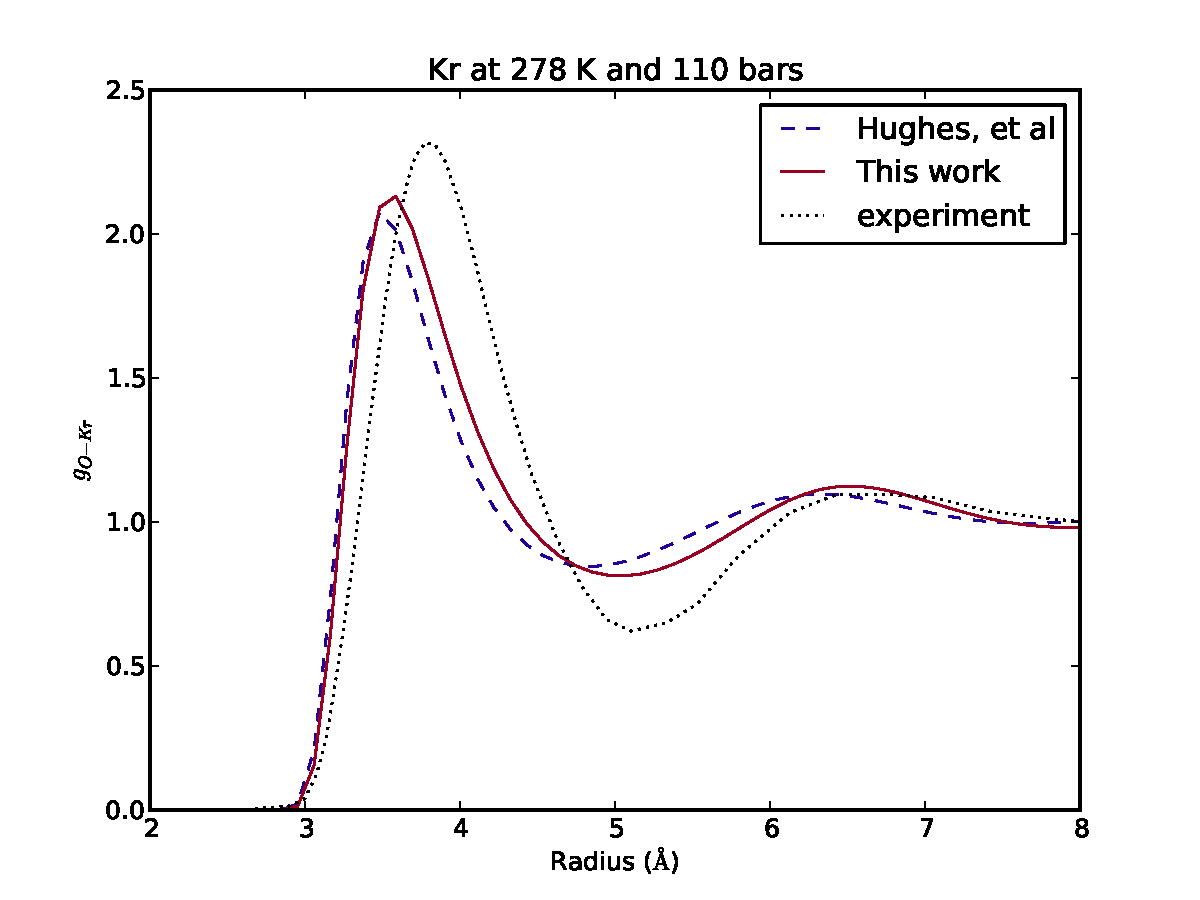
\includegraphics[width=3.5in]{figs/Kr-278K-densities}
\end{center}
\caption{ The Kr-O partial radial distribution function at low
  temperature ($5^\circ$ C) and high pressure (110 bar) in the limit
  of low concentration of krypton in water. The dashed blue line is
  computed using using the functional from \hughesetal, the solid red
  line is this work, and the black dotted line is from experiment
  \cite{bowron1998hydrophobic}. }
\label{fig:g-Kr}
\end{figure}

We have modified the classical DFT for water developed by
Hughes~\emph{et al.}~\cite{hughes2013classical} with the more accurate
radial distribution function at contact developed by Schulte~\emph{et
  al.}~\cite{schulte2012using}, which affects the predicted hydrogen
bonding between water molecules.  We found that while this
modification has a relatively mild effect on the free energy and
density profiles, it predicts fewer broken hydrogen bonds around
hard hydrophobic solutes and at aqueous interfaces.
%
The improved functional does indeed show better agreement with
experiment when used to compute the partial radial distribution
function of a krypton atom dissolved in water.

\clearpage

\section{Figures that are not included in the chapter (but could be)}

\begin{figure}
\begin{center}
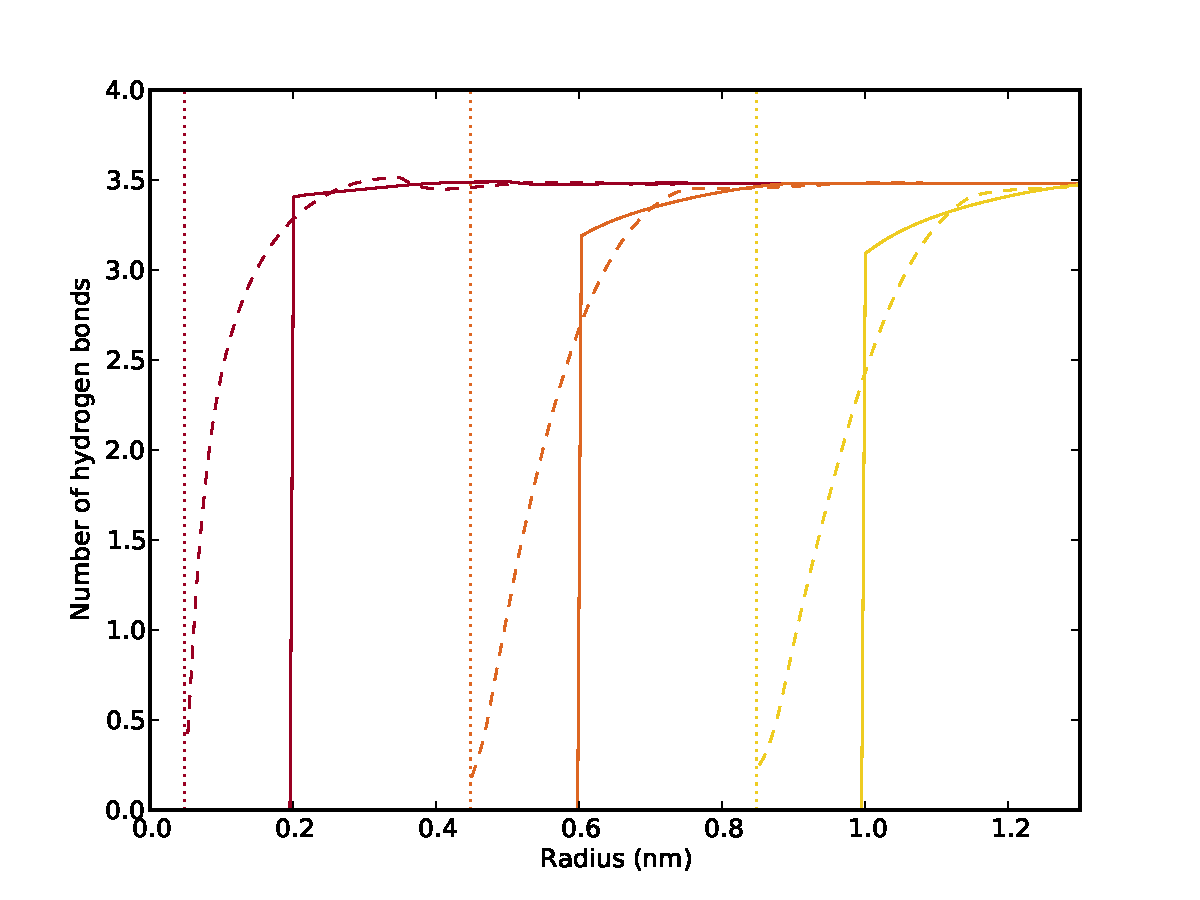
\includegraphics[width=3.5in]{figs/single-rod-X-plot}
\end{center}
\caption{ The average number of hydrogen bonds per molecule at
  distances from the center of hard rods of various
  radii. The solid lines are the results from using the assymetric
  $g_{\sigma}^A$, while the dotted lines are from Yu and Wu's $g_{\sigma}^{HS}$.}
\label{fig:single-rod-X}
\end{figure}

\begin{figure}
\begin{center}
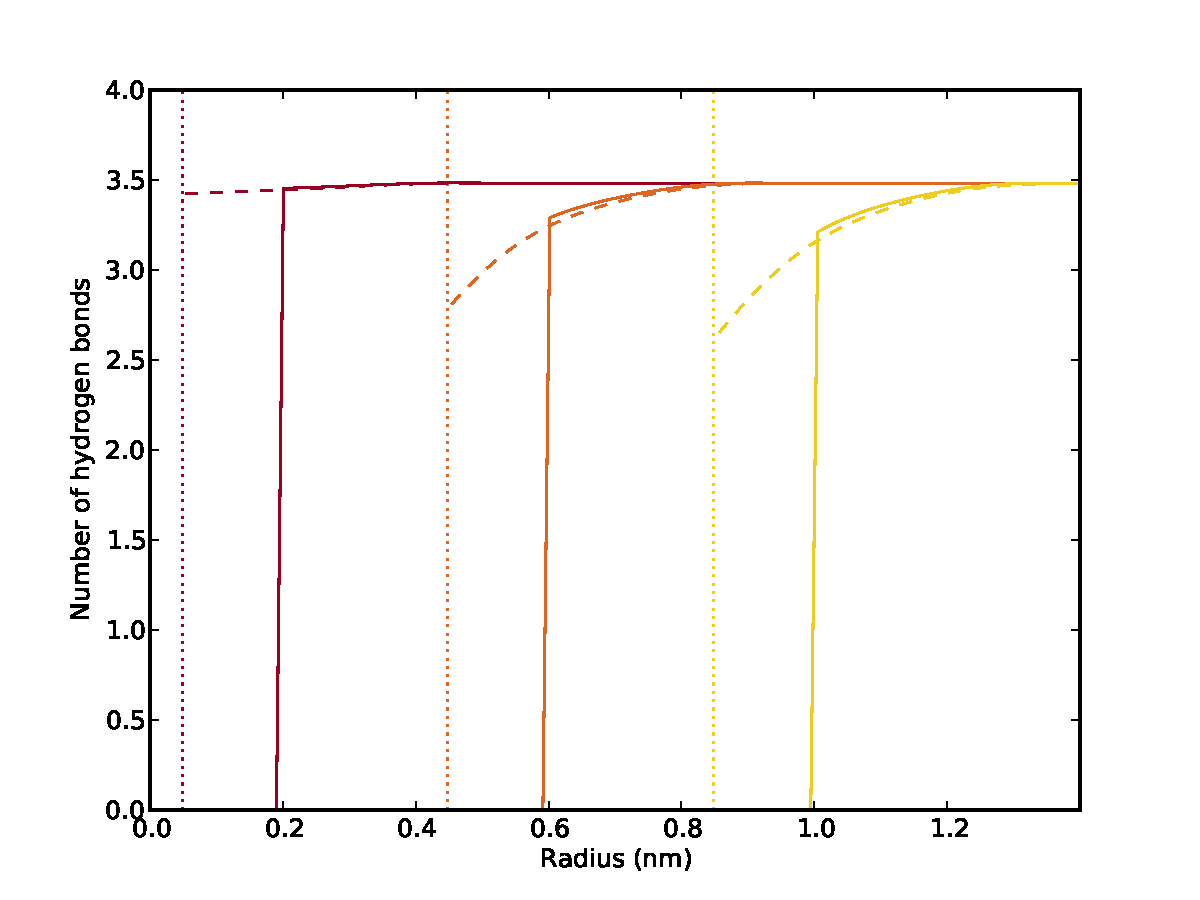
\includegraphics[width=3.5in]{figs/spheres-X-plot}
\end{center}
\caption{ The average number of hydrogen bonds per molecule at
  distances from the center of spherical cavities of various
  radii. The solid lines are the results from using the assymetric
  $g_{\sigma}^A$, while the dotted lines are from Yu and Wu's $g_{\sigma}$.}
\label{fig:spheres-X}
\end{figure}

\clearpage
\newpage
\chapter{Pair Distribution Function}
\label{chapter:pair}
%\newcommand{\red}[1]{{\bf \color{red} #1}}
%\newcommand{\green}[1]{{\bf \color{green} #1}}
%\newcommand{\blue}[1]{{\bf \color{blue} #1}}
%\newcommand{\cyan}[1]{{\bf \color{cyan} #1}}
%\newcommand{\rr}{\textbf{r}}
%\newcommand{\refnote}{\red{[ref]}}

%\newcommand{\fixme}[1]{\red{[#1]}}
\newcolumntype{d}[1]{D{.}{.}{#1}}
\newcommand{\newstuff}[1]{{\color{blue} #1}}

%\newcommand{\derivation}[1]{#1} % Use this to show all derivations in detail
%\newcommand{\derivation}[1]{} % Use this for nice pegagogical paper...
\newcommand{\davidsays}[1]{{\color{red} [\green{David:} \emph{#1}]}}
\newcommand{\jeffsays}[1]{{\color{red} [\cyan{Jeff:} \emph{#1}]}}
\newcommand{\pahosays}[1]{{\color{red} [\blue{Paho:} \emph{#1}]}}

\section{Introduction}
In this chapter we introduce an approximation for the pair
distribution function of the inhomogeneous hard sphere fluid. Our
approximation makes use of our recently published averaged pair
distribution function at contact, detailed in
chapter~\ref{chapter:contact}, which has been shown to accurately
reproduce the averaged pair distribution function at contact for
inhomogeneous density distributions. This approach achieves greater
computational efficiency than previous approaches by enabling the use
of exclusively fixed-kernel convolutions and thus allowing an
implementation using fast Fourier transforms. We compare results for
our pair distribution approximation with two previously published
works and Monte-Carlo simulation, showing favorable results.


Within standard liquid state theory, the perturbation theory treatment
of intermolecular interactions relies on the pair distribution
function of the reference fluid: $g_{HS}^{(2)}(\rr_1,\rr_2)$.  Unlike
the radial distribution function of a homogeneous fluid, there does
not currently exist a tractable form for the pair distribution
function of an inhomogeneous hard-sphere fluid, suitable for use in
constructing a density functional~\cite{gloor2007prediction,
jain2007modified}.

At its core, thermodynamic perturbation theory (TPT), sometimes referred to
as the high-temperature expansion, is an expansion of the
free energy in powers of a small parameter, which is the
product of a
pairwise attractive interaction with the inverse temperature $\beta$:
\begin{align}
  F &= F_0 + F_1 + \beta F_2 + \mathcal{O}(\beta^2)
\end{align}
where the terms $F_n$ are corrections to the free energy of order $n$
in the small interaction.  The first and largest term in this
expansion is
\begin{align}
  F_1[n(\rr)] &= \tfrac12 \iint \!\!
  g^{(2)}_{HS}(\rr_1,\rr_2)n(\rr_1)n(\rr_2)\Phi(|\rr_1-\rr_2|)
  d\rr_1d\rr_2
  \label{eq:mean-field}
\end{align}
where $g^{(2)}_{HS}(\rr_1,\rr_2)$ is the pair distribution function of
the hard-sphere reference fluid, and $\Phi(r)$ is the pair potential.
Formally, this requires the pair distribution function as a functional
of the density $n(\rr)$.  In Section~\ref{sec:gV}, we introduce
existing theoretical approaches for computing
$g^{(2)}_{HS}(\rr_1,\rr_2)$ given the external potential felt by the
hard spheres.  In Section~\ref{sec:gn}, we introduce existing
approximations for the hard-sphere pair distribution that are
expressed as a functional of the density distribution $n(\rr)$, which
is a form that is more directly useful in the construction of
classical density functionals---which are themselves expressed as a
functional of the density.

In this chapter, we introduce a new contact value approach
(CVA) to approximating the hard-sphere pair distribution function
which is suitable for use in the creation of classical density
functionals based on thermodynamic perturbation theory. The resulting
function is based on a fit to the radial distribution function that is
separable in a way that enables efficient evaluation of the
integral in Eq.~\ref{eq:mean-field}.

\section{Pair distribution from the external potential}\label{sec:gV}

Given the external potential $V(\rr)$ felt by a hard-sphere fluid,
there are several approaches that have been used to compute the pair
distribution function.  We review these approaches here.  The
classic (and earliest) approach for computing the pair distribution
function given the external potential is Percus' trick of treating one
sphere as an additional contribution to the external potential, and to
find the pair distribution function from the resultant equilibrium
density~\cite{hansen2006theory}.  This elegant approach lends itself
to computation \emph{using} DFT, and can be used to compute and plot the pair
distribution function, but requires a full free-energy minimization
\emph{for each position} $\rr_1$ in $g^{(2)}(\rr_1,\rr_2)$, and hence
would be prohibitively expensive as a tool in constructing a free
energy functional.

The canonical inhomogeneous configuration for the hard-sphere fluid is
the system consisting of a hard sphere at a hard wall.  In 1986,
Plischke and Henderson solved the pair distribution function of this
system using integral equation theory under the Percus-Yevick
approximation~\cite{plischke1986pair}.
%
Lado recently introduced a new and more efficient algorithm for
implementing integral equation theory for inhomogeneous fluids, which
computes $g^{(2)}(\rr_1,\rr_2)$~\cite{lado2009efficient}.  While this
approach is two orders of magnitude more efficient than previous
implementations, it remains a computationally expensive approach, and
unsuitable for repeated evaluation within a free-energy minimization
as required by DFT.

Another inhomogeneous configuration that is of interest is the
test-particle configuration, in which one hard sphere is fixed.  Where
the hard-wall is a surface with no curvature, the test-particle
configuration has a surface with curvature at the molecular length
scale.  In this case, the density gives the radial distribution
function---this is just Percus' trick---and the pair distribution
function of this inhomogeneous test-particle system gives the triplet
distribution function of the homogeneous fluid.  The triplet
distribution function of the homogeneous fluid has been computed by
Gonz\'alez \emph{et al.} using the test-particle approach with
\emph{two} spheres fixed~\cite{gonzalez1999test}.

\section{Pair distribution from the density}\label{sec:gn}

The alternative to specifying the external potential is to specify the
density distribution $n(\rr)$.  One may move between these
representations by either computing the external potential
corresponding to a given density of hard spheres by taking a
functional derivative of the hard-sphere free energy functional, or by
minimizing the free energy given an external potential.  However, in
general it is simplest to use an approach that makes use of the
natural variables, which in the case of classical density functional
theory is the density.

The most direct and rigorous approach to find the pair distribution
function given the density is to take a second functional derivative
of the hard-sphere free energy to find the direct correlation
function.  One can then solve the Ornstein-Zernike equation
numerically to find the pair distribution function.  This approach was
used by G{\"o}tzelmann \emph{et al.} to solve for the pair
distribution function near a hard wall using an early hard-sphere free
energy functional~\cite{gotzelmann1996structure}.  While this approach
is rigorous, solving the inhomogeneous Ornstein-Zernike equation
remains computationally challenging, although more efficient
approximate algorithms have been developed~\cite{paul2003variational}.
This approach, while appealing, remains unsuitable for use in the
construction of a classical density functional due to its significant
computational cost.

In addition to the above exact approach, there are a number of
analytic approximations for the inhomogeneous pair distribution
function, which extend the radial distribution function to
inhomogeneous scenarios.  These approximations differ both in what
density to use when evaluating the radial distribution function
$g(r;n)$, and in how to combine the radial distribution function
evaluated at these densities~\cite{toxvaerd1973statistical}.

Early approximations to the pair distribution function used the
density at one or two positions to determine the pair distribution
function.  There are three common approaches:
\begin{align}
  g^{(2)}(\rr_1,\rr_2) &\approx
  g\left(r_{12}; n\left(\frac{\rr_1+\rr_2}{2}\right)\right)
     & \text{midpoint} \\
  g^{(2)}(\rr_1,\rr_2) &\approx
  g\left(r_{12}; \frac{n(\rr_1)+n(\rr_2)}{2}\right)
     & \text{mean density} \\
  g^{(2)}(\rr_1,\rr_2) &\approx
  \frac{g(r_{12};n(\rr_1))+g(r_{12};n(\rr_2))}{2}
     & \text{mean function}\label{eq:mean-function}
\end{align}
These approaches have been successfully and widely used in treating
the surface tension of simple fluids~\cite{pressing2003surface,
  salter2008statistical, bongiorno1975modified,
  toxvaerd1976hydrostatic, kalos1977structure, carey2008gradient,
  osborn1980monotonic, mccoy1981comparison, barrett2006some}.  The
mean density approximation has also been quoted (as a goal) by recent
papers that proceed to make further
approximations~\cite{gloor2007prediction, gross2009density}.  However,
these approximations fail dramatically when applied to strongly
inhomogeneous systems such as a dense fluid at a solid surface.  Such
systems exhibit a strongly oscillatory density distribution, with
density peaks that can have local packing fractions greater than
unity, which cannot occur in the bulk reference system that defines
$g(r; n)$.  The above papers restrict themselves to the liquid-vapor
interface, which does not exhibit this pathology.

Non-pathological approaches use an average of the density over some
volume. Fischer and Methfessel introduce the
approximation~\cite{fischer1980born,harris1987comment}:
\begin{align}
  g^{(2)}(\rr_1,\rr_2) \approx g\left(r_{12}; n_3\left(\tfrac12
  (\rr_1+\rr_2)\right)\right)
  \label{eq:fischer}
\end{align}
where $n_3$ is an integral of the density over a spherical volume that
is now used as one of the fundamental measures in Fundamental
Measure Theory~\cite{rosenfeld1989free}:
\begin{align}
  n_3(\rr) = \int n(\rr')\Theta(\tfrac12 \sigma - |\rr-\rr'|) d\rr'
\end{align}
Equation~\ref{eq:fischer} is computationally awkward, because it
treats as special the midpoint $\tfrac12(\rr_1+\rr_2)$.  Moreover, the
approach of Fischer and Methfessel is intended to approximate the pair
distribution function only at contact, when the distance between
$\rr_1$ and $\rr_2$ is the hard-sphere diameter.
%
Tang \emph{et al.} employed an approximation for the pair distribution
function that is similar to that of Fischer and Methfessel, but with a
self-consistent weighted density computed with a weighting function that
is itself dependent on the weighted density~\cite{tang1991density}.
This weighted density was computed using the hard-sphere weighted
density of Tarazona, which was developed using the direct correlation
function of the homogeneous hard-sphere fluid~\cite{tarazona1985free}.

Sokolowski and Fischer addressed the shortcomings of the theory of
Fischer and Methfessel by modifying this approach to use density
averages centered on the two points $\rr_1$ and $\rr_2$:
\begin{align}
  g^{(2)}(\rr_1,\rr_2) \approx g\left(r_{12};
  \tfrac12(\bar{n}(\rr_1)+\bar{n}(\rr_2))\right)
  \label{eq:sokolowski}
\end{align}
where their averaged density $\bar{n}(\rr)$ given by
\begin{align}
  \bar{n}(\rr) \equiv \frac{3}{4\pi (0.8\sigma)^3}\int n(\rr')\Theta(0.8\sigma - |\rr-\rr'|) d\rr'
\end{align}
is the density averaged over a sphere with diameter
$0.8\sigma$~\cite{sokolowski1992role}.  The value 0.8 in this formula
was arrived at by fitting to Monte Carlo simulation.  Although
Eq.~\ref{eq:sokolowski} has the advantage of only involving
density averages at the points at which the pair distribution function
is desired, it remains sufficiently computationally cumbersome that it
has only been used in two papers studying the one-dimensional liquid vapor
interface~\cite{wadewitz2000application, winkelmann2001liquid}.
Because it cannot be written as a single-site convolution, this
approach is particularly computationally demanding when applied to
systems featuring inhomogeneity in more than one dimension.

In Chapter~\ref{chapter:contact}, we introduce a functional that gives
a good approximation for the pair distribution function averaged over
positions $\rr_2$ that are in contact with $\rr_1$, defined as:
\begin{align}
  g_\sigma(\rr_1) &\equiv \frac{ \int g^{(2)}(\rr_1,\rr_2) \delta(\sigma -|\rr_1-\rr_2|)n(\rr_2)
    d\rr_2 }{ \tilde{n}(\rr_1)  }
\end{align}
where the weighted density $\tilde{n}(\rr_1)$ is defined by:
\begin{align}
  \tilde{n}(\rr) &\equiv \int n(\rr') \delta(\sigma -|\rr - \rr'|)d\rr'.
\end{align}
In Chapter~\ref{chapter:contact} we use the contact-value theorem to derive the exact formula:
\begin{align}
  g_\sigma(\rr)% &= \frac{\ncontact(\rr)}{n_A(\rr)} \\
  &= \frac12 \frac{1}{k_BT n(\rr) \tilde{n}(\rr)} \frac{\delta
    F_{HS}}{\delta \sigma(\mathbf{r})} \label{eq:gsigma-exact}
\end{align}
where $\sigma(\rr)$ is the diameter of hard spheres located at
position $\rr$, and $F_{HS}$ is the Helmholtz free energy of the
hard-sphere fluid.  The functional derivative of the free energy with
respect to the hard-sphere diameter in Eq.~\ref{eq:gsigma-exact} requires
that we be able to evaluate the change in free energy resulting from a
change in the diameter of specifically the hard spheres located at
position $\rr$.  This somewhat unusual construction is mathematically
straightforward within Fundamental Measure Theory
(FMT)~\cite{rosenfeld1989free}.  We employ the White Bear variation of
the FMT free energy functional~\cite{roth2002whitebear}, which
provides an excellent approximation for this averaged value of the
pair distribution function at contact for a variety of interfaces, and
over a wide range of densities.

  %% \jeffsays{We had a clarifying paragraph below but I don't think
  %% it's needed anymore, at least not here.  The explanation up until
  %% this point is moving along fine and I don't think it needs
  %% clarification.}

%% \jeffsays{My attempt at this paragraph:} To be
%% clear we note that for our purposes in this work we use the hard
%% sphere free energy twice.  It is first minimized to find $n(\rr)$ and
%% then its functional derivative is used to find $g_\sigma(\rr)$.  In
%% actual application of perturbation theory the hard sphere free energy
%% would be used only to find $g_\sigma(\rr)$, which would in turn be
%% used in the approximation for $g^{(2)}(\rr_1,\rr_2)$ that would appear
%% in a perturbation term.  The free energy that would be minimized to
%% find $n(\rr)$ in this case would be the total free energy and not the
%% hard sphere free energy.


\section{Contact value approach}
In the approaches for the pair distribution function
mentioned above, the radial distribution function used in the
approximation was dependent upon the density averaged over some
volume.  We seek to achieve greater accuracy by making use of a
function dependent upon our averaged $g_{\sigma}(\rr)$ discussed
above, which holds more information about an inhomogeneous system than
does a simple convolution of the density.
%
We construct the CVA with the average of two radial distribution
functions, evaluated at the distance between the two points, that are
themselves functions of the averaged pair distribution function at contact
$g_{\sigma}(\rr)$ evaluated at the two points:
\begin{align}
  g^{(2)}(\rr_1,\rr_2) = \frac{g(r_{12}; g_\sigma(\rr_1)) +
    g(r_{12}; g_\sigma(\rr_2))}{2}. \label{eq:g2-our-mean}
\end{align}
This CVA for $g^{(2)}(\rr_1,\rr_2)$ is
constructed to reproduce the exact value for the integral:
\begin{align}
  F_1^{\text{contact}} &= \tfrac12 \iint
  g^{(2)}_{HS}(\rr_1,\rr_2)n(\rr_1)n(\rr_2)\delta(|\rr_1-\rr_2|-\sigma)
  d\rr_1d\rr_2
  \label{eq:mean-field-contact}
\end{align}
which is the mean-field correction to the free energy (see
Eq.~\ref{eq:mean-field}) for a purely contact interaction.

The CVA requires the radial distribution function expressed as a
function of $r$ and $g_\sigma$.
%
%% \fixme{One approach to constructing $g(r;g_\sigma)$ is to compute $n$
%%   from $g_\sigma$ (using e.g. the Carnahan-Starling formula for
%%   $g_\sigma$) and then find $g(r;n)$ using either some approximate
%%   functional form (e.g. Percus-Yevick) or Monte Carlo simulation
%%   results.}
%
We construct a functional form for $g(r, g_\sigma)$ that allows for
improved computational efficiency.  We introduce the general form that
allows for this efficiency in Section~\ref{sec:efficient}, and we
detail our specific approximation for $g(r,g_\sigma)$ that uses this
general form in Section~\ref{sec:separable-fit}.
%
%% When evaluating the approximations of earlier works described in
%% Section~\ref{sec:gn} for comparison, we use interpolated
%% Monte Carlo results for $g(r;n)$.


\newcommand\maxrfit{4}
\newcommand\maxerr{0.2}
\newcommand\etamaxerr{0.45}
\newcommand\rmaxerr{3.7}
\newcommand\chisq{2.5}
\newcommand\kappatable{
  \left(
  \begin{array}{c d{3} d{3} d{3} d{3}}
    -1.754 & 0.027 & 0.838 & -0.178 \\
    -2.243 & 4.403 & -2.48 & 0.363 \\
    0.207 & 0.712 & -1.952 & 1.046 \\
    -0.002 & -0.164 & 0.324 & -0.162 \\
  \end{array}
  \right)
}
\newcommand\alphaval{-0.002}


\section{Making the CVA efficient}
\label{sec:efficient}
The existing approaches to approximating the pair distribution
function outlined in Section~\ref{sec:gn} have not been widely used in
the construction of density functionals based on thermodynamic
perturbation theory, largely due to their computational complexity.
While our CVA provides only an incremental improvement in accuracy,
its construction enables significant gains in computational
efficiency, allowing for practical application in density functionals.
We achieve this gain by developing a \emph{separable} fit to the radial
distribution function of the hard-sphere fluid (see
Section~\ref{sec:separable-fit} for details).  This separable fit is
of the form
\begin{align}
  g(r; g_\sigma) &= \sum_{i} a_i(r) b_i(g_\sigma)
\end{align}
where the notable aspect is that the radial distribution function is
written as a sum of terms that are each a simple product of a function
of radius with a function of $g_\sigma$.  This enables us to write
integrals---such as Eq.~\ref{eq:mean-field}---that are linear in the
pair distribution function as a summation of fixed-kernel
convolutions, which may be efficiently computed using Fast Fourier
Transforms (FFTs).

\newcommand\Vcell{V_{\textit{cell}}}
\newcommand\Vinteraction{V_{\Phi}}

Computation of the free energy correction from Eq.~\ref{eq:mean-field}
for a periodic system by direct integration requires a nested
integration over the volume of the system~$\Vcell$, and the volume
over which the interaction is nonzero~$\Vinteraction$.  Thus the cost
of computation scales as
$\mathcal{O}\left(\frac{\Vcell\Vinteraction}{\Delta V^2}\right)$ where
$\Delta V$ is the volume resolution of the computational grid.  Direct
integration is the most efficient algorithm when using the existing
functionals for $g^{(2)}(\rr_1,\rr_2)$ described in
Section~\ref{sec:gn}.  The one exception is the ``mean-function''
approximation (Eq.~\ref{eq:mean-function}), which could in principle
be made more efficient using the same technique we describe here.
Because the CVA allows the integral in Eq.~\ref{eq:mean-field} to be
written as a sum of fixed-kernel convolutions, it can be computed
without a nested integral, at the cost of performing a few FFTs.  This
approach scales as $\mathcal{O}\left(\frac{\Vcell}{\Delta
  V}\log\frac{\Vcell}{\Delta V}\right)$, as do most widely used DFT
functionals such as FMT~\cite{rosenfeld1989free, roth2002whitebear}.
%
With this scaling, when examining systems with long interaction
distances or high resolution---which is often necessary when working
with hard-sphere functionals---the CVA has the potential to be far
more efficient than existing methods.

\begin{figure}
  \centering
  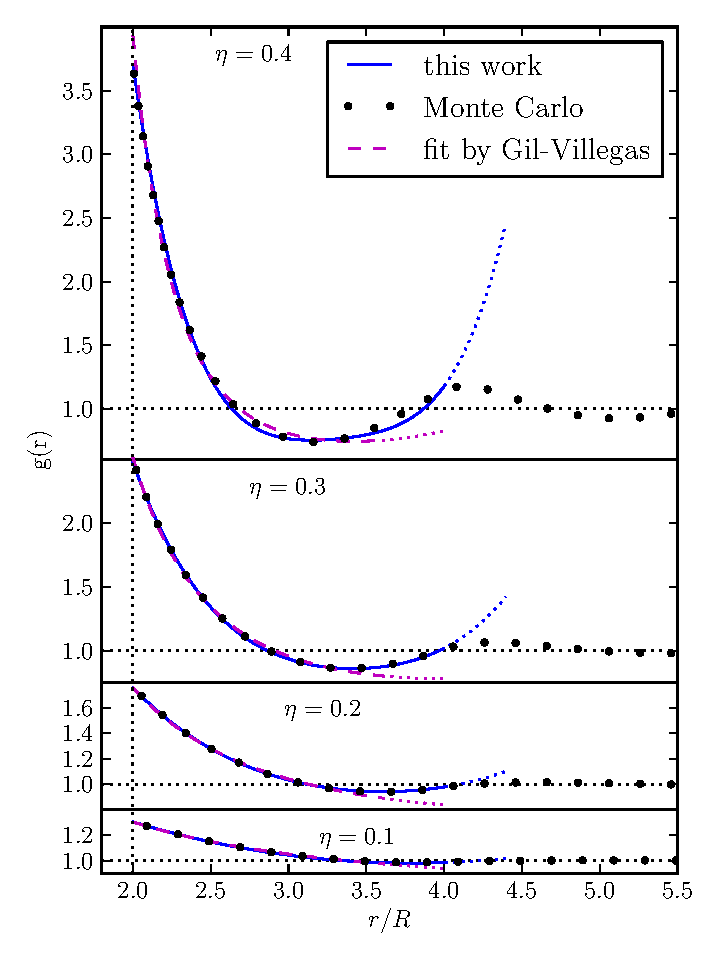
\includegraphics[width=13cm]{figs/short-range-ghs-alt}
  \caption{Plot of the hard-sphere radial distribution function of the
    homogeneous fluid at several values for packing fraction $\eta$. The
    blue lines show our separable fit, the black dots show the true
    radial distribution function $g(r)$ as found from Monte Carlo
    simulation, and the dashed lines are results of the
    Gil-Villegas fit~\cite{gil1997statistical}.  The dotted extension
    of each fitted curve indicates the value of the function outside
    of the fitted region.  }\label{fig:radial-distribution}
\end{figure}

To see how we obtain this improved scaling, we examine the
lowest-order correction in TPT, given by Eq.~\ref{eq:mean-field}.  The
two terms that are averaged in Eq.~\ref{eq:g2-our-mean} give equal
contributions to the integral
\begin{align}
  F_1^{\textit{CVA}} &= \tfrac12 \!\! \iint \!\!
  g(r_{12};g_\sigma(\rr_2))n(\rr_1)n(\rr_2)\Phi(|\rr_1-\rr_2|)
  d\rr_1d\rr_2.
\end{align}
When we introduce the separable form for $g(r_{12};g_\sigma)$ we can
further simplify this integral as
\begin{align}
  F_1^{\textit{CVA}} \! = \!
  \sum_i \!\tfrac12 \!\! \int \!\! n(\rr_1) \!\!
                            \int \!\!\!
                            %\big(
                            a_i(r_{12})\Phi(r_{12})
                            %\big)
                            %\big(
                            b_i(
g_\sigma(\rr_2))n(\rr_2)
                            %\big)
  d\rr_2d\rr_1
\end{align}
where the functional is written as a summation of integrals of simple
convolutions in three dimensions.  Thus, each of these integrals may
be computed in $\mathcal{O}(N\log N)$ time, where $N$ is the number of
grid points in the computational cell.  This is the same scaling as is
required to compute the fundamental measures such as $n_3$ which are
used in FMT.

\section{A separable fit for the radial distribution function}\label{sec:separable-fit}

Having settled on the basic structure of our function, we further
refine it by performing a separable fit to the radial distribution
function from Monte Carlo simulation.  We focus our fit on
the range of distances $r_{12} \le \maxrfit R$.  This range is
relevant to the widely used \cite{chapman1989saft,
  muller2001molecular, tan2008recent} Statistical
Associating Fluid Theory of Variable Range (SAFT-VR) free energy with
square-well dispersive attraction developed by Gil-Villegas \emph{et
  al.}~\cite{gil1997statistical}.
%
Although we consider this range of radii particularly interesting,
this is not a fundamental limit of the approach, as one could readily
extend the fit to larger radii by including additional fitting
parameters.
%
For comparison, in Fig.~\ref{fig:radial-distribution} we plot our fit,
Monte-Carlo data, and the radial distribution function of Gil-Villegas
\emph{et al.}, which we have extracted from their approximation for
the first term in the dispersion free energy given by
Eq.~\ref{eq:mean-field}.

For ease of implementation and future extension to larger radii, we
fit the radial distribution function using a fourth-order polynomial.  We constrain
our functional form such that $g(r; g_\sigma)$ reduces to $g_\sigma$
at contact and approaches $g(r)=1$ in the low-density limit.
Incorporating these constraints we have the functional form
\begin{align}
  g(r;g_\sigma) &=
  g_\sigma + \sum_{i=1}^{4} \sum_{j=1}^{4} \kappa_{ij} (g_\sigma - 1)^i
  \left(\tfrac{r}{\sigma}-1\right)^j,
  \label{eq:fit-form}
\end{align}
where the matrix $\kappa_{ij}$ is determined from a least-squares
fit to Monte Carlo data for the radial distribution function, over the
range $2R \le r \le \maxrfit R$, and for packing fractions $\eta \le
0.45$.  The resulting parameters are displayed in
Table~\ref{tab:kappa}.  The maximum error in $g(r)$ within this
range is \maxerr, which occurs at $\eta = \etamaxerr$ and $r =
\rmaxerr R$.  Fig.~\ref{fig:radial-distribution} displays
our approximation at just under half of the densities that were
included in the fit.

\begin{table}
  \begin{align*}
    \kappa &= \kappatable
  \end{align*}
  \caption{The fitted $\kappa_{ij}$ matrix.
    %% In addition to these 12 parameters, we also optimized the
    %% exponetial decay constant $\alpha=\alphaval$.za
    %% Note that the first column of $\kappa$ corresponds to $j=1$
    %% while the first row corresponds to $i=1$ in
    %% Eq.~\ref{eq:fit-form}.
  }\label{tab:kappa}
\end{table}

\newcommand{\plotcomp}[1]{The top halves of
  these figures show the results of Monte Carlo simulations, while the
  bottom halves show the CVA, truncated beyond the range of the fit.
  On the right are plots of #1 on the
  paths illustrated in the figures to the left.  These plots compare
  the CVA (blue solid line), Monte Carlo results (black circles), the
  results of Sokolowski and Fischer (red dashed
  line)~\cite{sokolowski1992role}, and those of Fischer and Methfessel
  (green dot-dashed line)~\cite{fischer1980born}.  The latter is only
  plotted at contact, where it is defined}

\begin{figure*}
  \begin{subfigure}{\textwidth}
    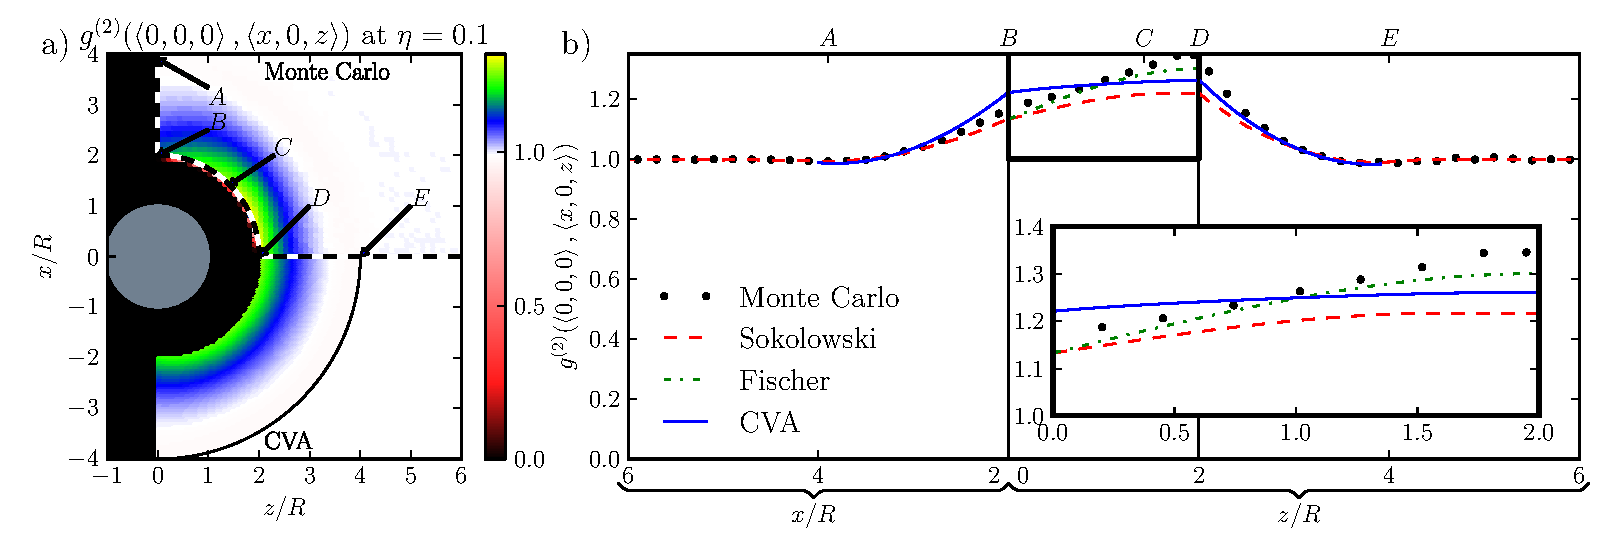
\includegraphics[width=\linewidth]{figs/pair-correlation-pretty-1.pdf}
    \vspace{-0.6cm}
  \end{subfigure}
  \begin{subfigure}{\textwidth}
    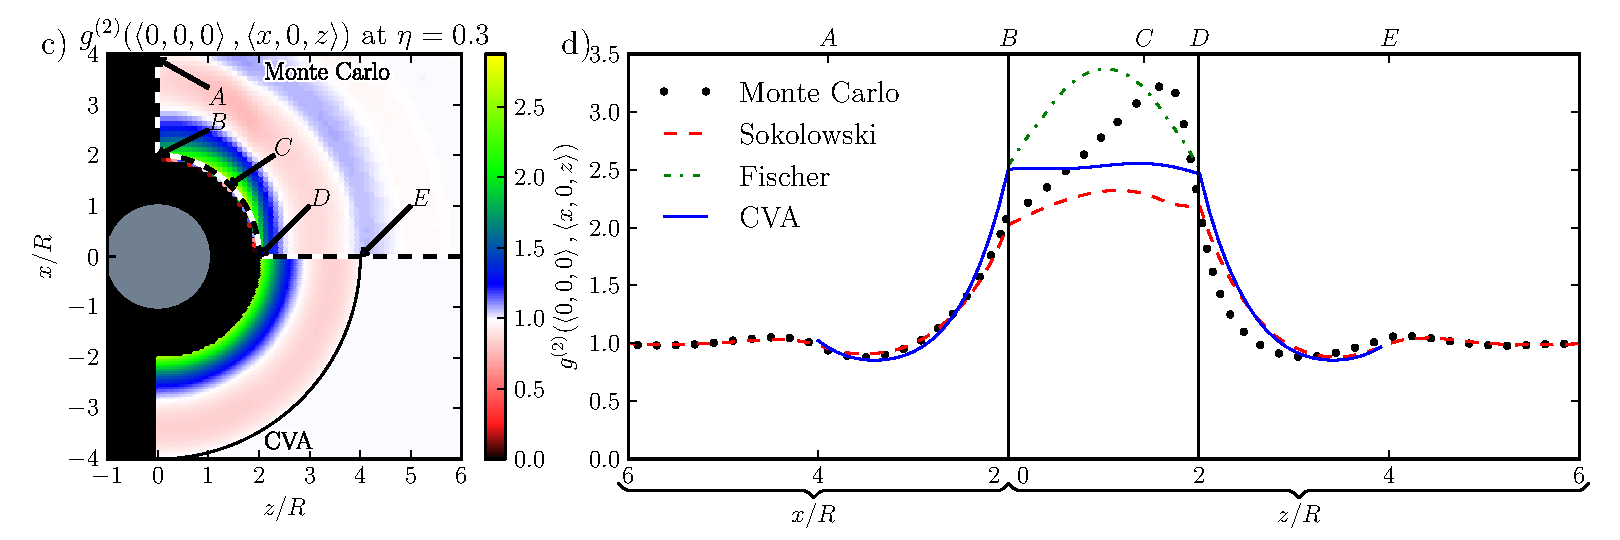
\includegraphics[width=\linewidth]{figs/pair-correlation-pretty-3.pdf}
    \vspace{-0.6cm}
  \end{subfigure}
  \caption{The pair distribution function near a hard wall, with
    packing fractions of 0.1 and 0.3 and $\rr_1$ in contact with the
    hard wall.  On the left are 2D plots of $g^{(2)}(\rr_1,\rr_2)$ as
    $\rr_2$ varies. \plotcomp{$g^{(2)}(\rr_1,\rr_2)$}.}
  \label{fig:pair-distribution}
\end{figure*}

\section{Results}

\subsection{Pair distribution function}

%% \begin{figure}
%%   \includegraphics[width=\columnwidth]{figs/pair-correlation-pretty-2.pdf}
%%   \caption{\paircaption{0.2}}\label{fig:pair-distribution-2}
%% \end{figure}
% \begin{figure}
%   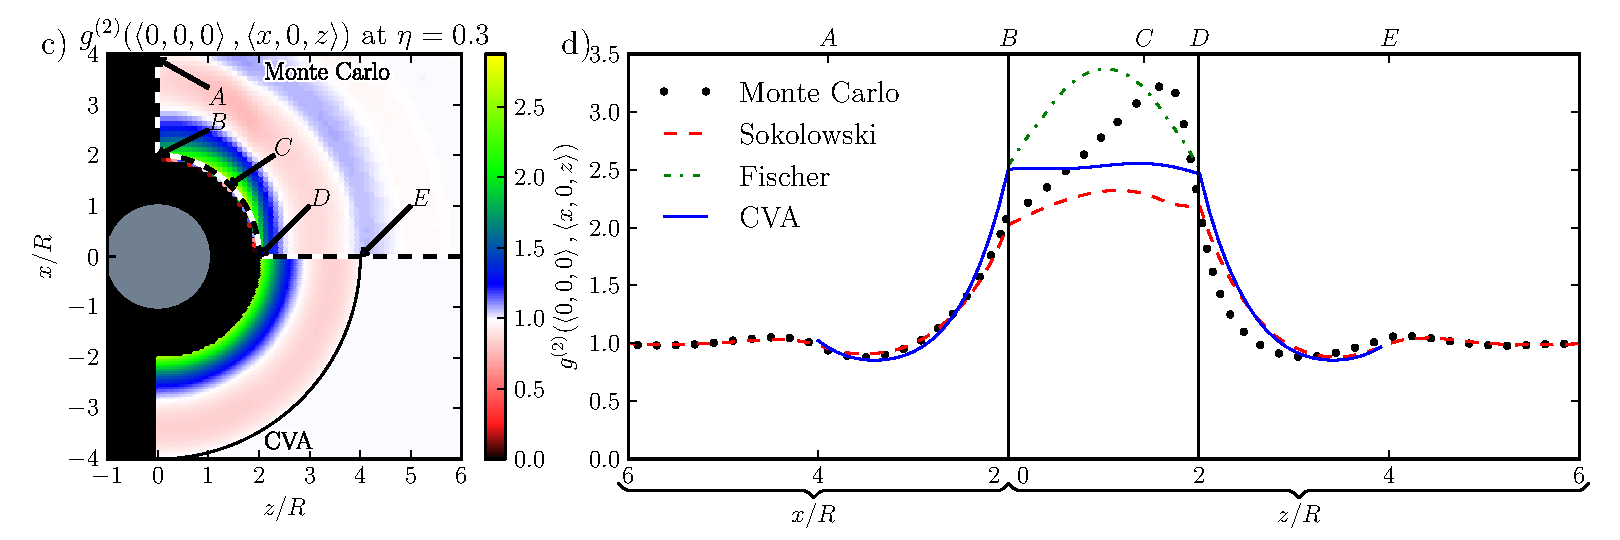
\includegraphics[width=\columnwidth]{figs/pair-correlation-pretty-3.pdf}
%   \caption{\paircaption{0.3}}\label{fig:pair-distribution-3}
% \end{figure}
%% \begin{figure}
%%   \includegraphics[width=\columnwidth]{figs/pair-correlation-pretty-4.pdf}
%%   \caption{\paircaption{0.4}}\label{fig:pair-distribution-4}
%% \end{figure}

We begin by examining the pair distribution function near a hard wall,
with a focus on the case where one of the two spheres is in contact
with the hard wall.  Figures~\ref{fig:pair-distribution}a
and~\ref{fig:pair-distribution}c compare the results of the CVA with
Monte Carlo simulations at packing fractions of 0.1 and 0.3
respectively. We see reasonable agreement at the lower density, with a flatter angular
dependence when the two spheres are in contact.  At the higher
density, we see significant structure developing in the simulation
results that is not reflected in our approximation.

\begin{figure*}
  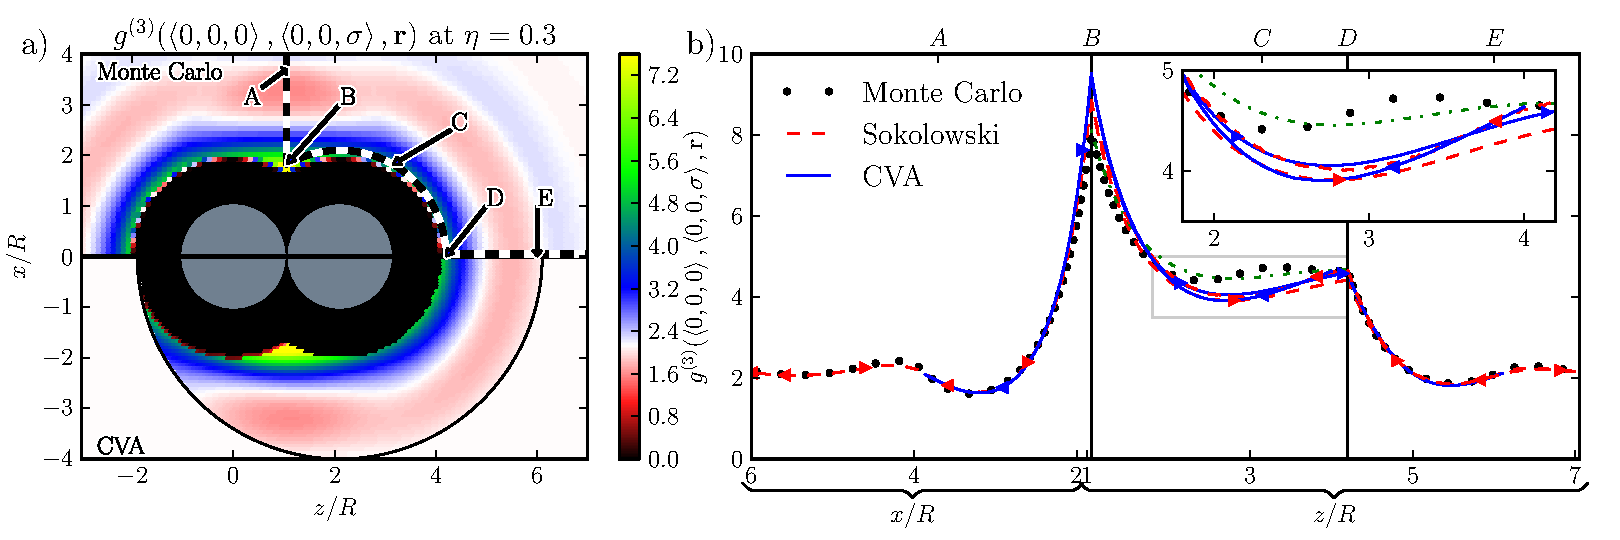
\includegraphics[width=\textwidth]{figs/triplet-correlation-pretty-contact-3.pdf}
  \vspace{-0.7cm}
\\
  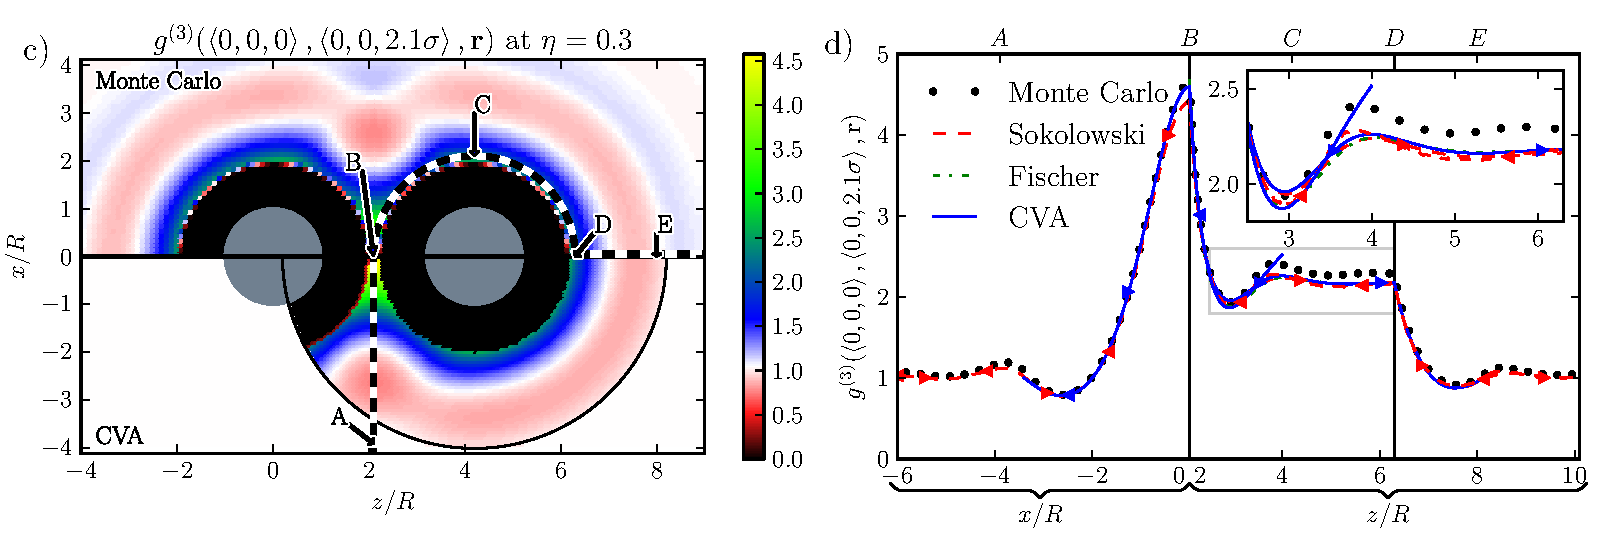
\includegraphics[width=\textwidth]{figs/triplet-correlation-pretty-inbetween-3.pdf}
  \vspace{-0.7cm}
  \caption{The triplet distribution function
    $g^{(3)}(\rr_1,\rr_2,\rr_3)$ at packing fraction 0.3, plotted when
    $\rr_1$ and $\rr_2$ are in contact (a,b) and when $\rr_1$ and
    $\rr_2$ are separated by a distance $2.1\sigma$ (c,d). On the left
    are 2D plots of $g^{(3)}(\rr_1,\rr_2,\rr_3)$ as $\rr_3$
    varies. %\plotcomp{$g^{(3)}(\rr_1,\rr_2,\rr_3)$}.
%
    The top halves of these figures show the results of Monte Carlo
    simulations, while the bottom halves show the CVA, truncated
    beyond the range of the fit.  On the right
    are plots of $g^{(3)}(\rr_1,\rr_2,\rr_3)$ on the paths illustrated
    in the figures to the left.
%
    We also plot these curves along a left-right mirror image of this
    path.  The data for the right-hand paths (as shown in the 2D
    images) are marked with right-pointing triangles, while the
    left-hand paths are marked with left-pointing triangles.
%
    %% The line styles are the same as in
    %% Fig.~\ref{fig:pair-distribution}.
  }
  \label{fig:triplet-contact-distribution}
\end{figure*}

Figures~\ref{fig:pair-distribution}b and~\ref{fig:pair-distribution}d
show the pair distribution function as plotted along paths illustrated
in Figures~\ref{fig:pair-distribution}a
and~\ref{fig:pair-distribution}c.  These plots compare the CVA with
Monte Carlo results, as well as the approximations of Sokolowski and
Fischer~\cite{sokolowski1992role} and of Fischer and
Methfessel~\cite{fischer1980born} at the same packing fractions of 0.1
and 0.3.  The approach of Fischer and Methfessel is only defined when
the two spheres are in contact, and is therefore only plotted on that
segment of the path.  As an input to the previous approximations we
use the hard sphere radial distribution function found with Monte
Carlo simulation, interpolated as necessary. We find that both
previous approximations to the pair distribution function predict
stronger angular dependence of the pair distribution function at
contact than this work.  The previous approximations each have a
systematic error at contact---either too high or too low.  In
contrast, our errors at contact have a tendency to cancel when used in
a perturbation expansion.  At higher densities, the approximation of
Fischer and Methfessel requires evaluating the radial distribution
function at densities significantly higher than the freezing density,
which poses numerical difficulties when using the radial distribution
function from simulation.  When the two points $\rr_1$ and $\rr_2$ are
both more than a radius away from contact, we find that any of these
approaches gives a reasonable prediction.

\subsection{Triplet distribution function}

Just as the radial distribution function of a homogeneous fluid may be
computed from the density of an inhomogeneous one using Percus'
test-particle trick, the triplet distribution function of a
homogeneous system can be computed using an approximation of the pair
distribution for an inhomogeneous fluid, such as we have
developed. The triplet distribution function of a homogeneous fluid
with density $n$ is given by:
\begin{align}
    g^{(3)}(\rr_1,\rr_2,\rr_3) =
    \frac{n_{\textrm{TP}(\rr_1)}(\rr_2)
      n_{\textrm{TP}(\rr_1)}(\rr_3)}{n^2}
    g^{(2)}_{\textrm{TP}(\rr_1)}(\rr_2,\rr_3)
\end{align}
where the $\textrm{TP}(\rr_1)$ subscript indicates quantities computed for
the inhomogeneous density configuration in which one sphere (the
``test particle'') is fixed
at position $\rr_1$.  This method treats one of the three
positions---the location of the test particle---differently from the
other two, which means that a poor approximation to the pair distribution
function may break the symmetry between $\rr_1$ and $\rr_2$ which is
present in the true triplet distribution function.

Figures~\ref{fig:triplet-contact-distribution}a
and~\ref{fig:triplet-contact-distribution}c compare the triplet
distribution function at a packing fraction of 0.3 computed using the
CVA with results from Monte Carlo simulations. In
Figure~\ref{fig:triplet-contact-distribution}a the spheres at $\rr_1$
and $\rr_2$ are in contact; in
Figure~\ref{fig:triplet-contact-distribution}c they are spaced so that
a third sphere can just fit between them; and in both figures $\rr_3$
is varied. The test-particle position for the CVA in each case is
$\rr_1$, which is on the left-hand side of the figure. As before, we
see reasonable agreement with simulation. Also, the Monte Carlo
results have the expected left-right symmetry, while the CVA has a
small asymmetry introduced with the test particle due to errors in the
pair distribution function.

Figures~\ref{fig:triplet-contact-distribution}b
and~\ref{fig:triplet-contact-distribution}d show the triplet
distribution function as plotted along the paths illustrated in
Figures~\ref{fig:triplet-contact-distribution}a
and~\ref{fig:triplet-contact-distribution}c.  We also plot the
results along a left-right mirror image path, corresponding to
swapping $\rr_1$ and $\rr_2$. The two mirror-image paths are
distinguished by arrows (triangles) along the curves, with right-facing arrows
indicating the paths shown in
Figures~\ref{fig:triplet-contact-distribution}a and
\ref{fig:triplet-contact-distribution}c, and left-facing arrows
indicating the mirror image path.  As the work of
Fischer and Methfessel is only defined when $\rr_2$ and $\rr_3$ are in
contact, we only plot it along the
central portion of the path, which is in contact with $\rr_2$, and arrows
are omitted.
%
All methods tested perform similarly over their range of validity.

\begin{figure}
  \begin{subfigure}{.9\columnwidth}
    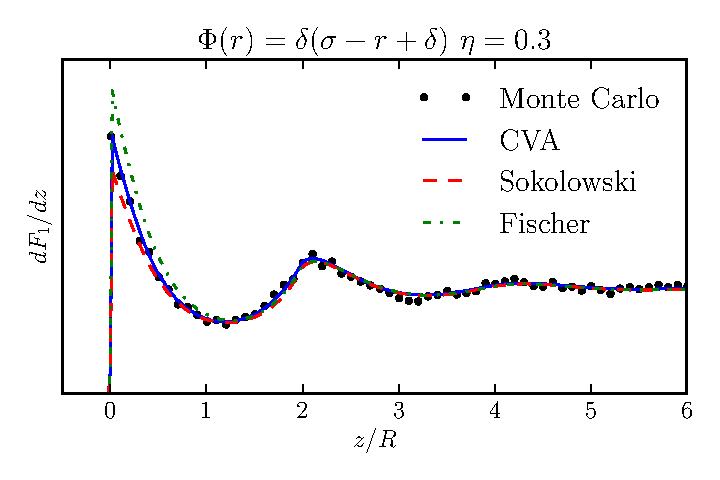
\includegraphics[width=\columnwidth]{figs/dadz-3-2.pdf}
    \vspace{-0.8cm}
    \caption{Sticky hard-sphere fluid}\label{fig:dadz-delta}
  \end{subfigure}
  \begin{subfigure}{.9\columnwidth}
    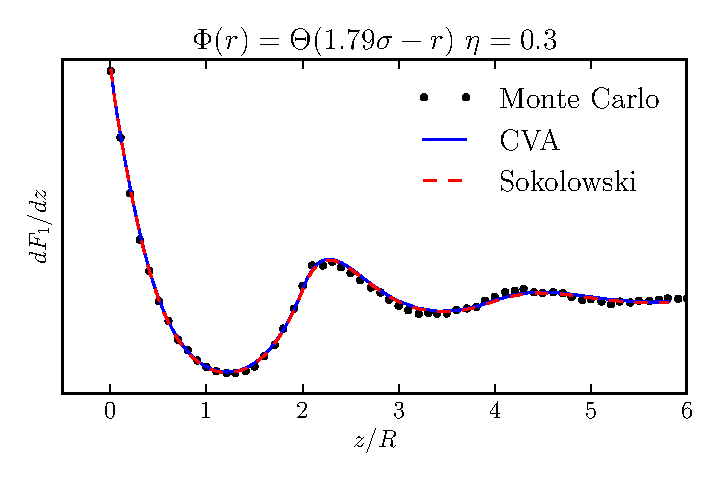
\includegraphics[width=\columnwidth]{figs/dadz-square-well-3.pdf}
    \vspace{-0.8cm}
    \caption{Hard-core square well fluid}\label{fig:dadz-square-well}
  \end{subfigure}
  \caption{Plot of $\frac{dF_1}{dz}$ near a hard wall, with arbitrary
    vertical scale.  (a) shows a
    sticky hard-sphere fluid defined by a pair potential
    $\delta(\sigma-r+\delta)$ where $\sigma$ is the hard-sphere
    diameter, and $\delta$ is an infinitesimal distance; and (b) shows a
    square well fluid defined by a pair potential $\Theta(1.79
    \sigma-r)$.
  }
  \label{fig:dadz}
\end{figure}

\section{Accuracy in thermodynamic perturbation theory}

A particularly relevant quantitative test of a pair distribution
function is how well it predicts the interaction energy due to a pair
potential.  To this end, we have computed the error in the first term
in a high-temperature perturbation expansion $F_1$
for two typical pair potentials.  In order to focus on effects at the
interface, we have defined a position-dependent pair interaction
energy as
\begin{align}
  \frac{dF_1}{dz} &=
  \tfrac12 \int g^{(2)}_{HS}(\rr,\rr')n(\rr)n(\rr')\Phi(|\rr-\rr'|)
  d\rr'\, dxdy\label{eq:da1}
\end{align}
which gives the contribution to the mean-field free energy due to
molecules located in a plane of fixed $z$.

We plot this quantity for two representative pair potentials near a
hard wall in Fig.~\ref{fig:dadz}.  We have chosen to illustrate a
delta-function interaction at contact (i.e. ``sticky hard spheres''),
and a hard-core square-well fluid, with the length-scale of
interaction taken from the optimal SAFT model for water found by Clark
\emph{et al.}~\cite{clark2006developing}.  These pair potentials
represent both a very short-range interaction and a medium-range
interaction.

Figure~\ref{fig:dadz-delta} shows the results for the sticky
hard-sphere fluid.  The CVA is constructed to produce this result
exactly, provided the averaged pair distribution function at contact
from Schulte~\cite{schulte2012using} is exact.  As expected, we see
excellent agreement with the Monte Carlo simulation results, while the
approximations of Fischer and Sokolowski each show deviations near the
interface.  Figure~\ref{fig:dadz-square-well} shows the same curve
from Eq.~\ref{eq:da1} for the square-well fluid.  In this case both
the CVA and Sokolowski's approximation give excellent agreement with
simulation.

\section{Conclusion}

We have introduced and tested the contact value approach for the pair
distribution function $g^{(2)}(\rr_1,\rr_2)$ of the inhomogeneous
hard-sphere fluid.  The pair distribution function plays a key role in
thermodynamic perturbation theory, which is widely used in the
construction of classical density functionals.  The CVA---unlike
existing approximations---is suitable for use in classical density
functionals based on perturbation theory, as it may be efficiently
computed using exclusively fixed-kernel convolutions.  We have tested
this function at a hard wall and near a single fixed hard sphere, and
find that it gives excellent agreement with simulation.  Tests of the
pair distribution function in integrals that arise in thermodynamic
perturbation theory suggest that the CVA is accurate for attractions
up to the distance to which the radial distribution function is fit,
and is a significant improvement over existing approximations near
contact.  But most importantly, the computational cost of using the
CVA in a classical density functional scales much more favorably than
existing methods in high resolution computations.

\clearpage

\clearpage
\newpage

\chapter{Conclusion}
Well folks!  That about wraps up our show for tonight!

I don't know what I should say in the conclusion.


\bibliography{THESIS}{}
\bibliographystyle{unsrt}


\appendix
\chapter{First stuff in the appendix}
\label{chapter:appendix}
The expression for the asymmetric correlation function
$g_\sigma^A(\rr)$ (Equation~\ref{eq:g-A-exact}) involves the
functional derivative $\frac{\delta A_{HS}}{\delta
  \sigma(\mathbf{r})}$.  In this appendix we will explain how this
derivative is evaluated.  We begin by applying the chain rule in the
following way:
  \begin{align}
    \frac{\delta A_{HS}}{\delta \sigma(\mathbf{r})} &=
    \int \left(
    \sum_\alpha
    \frac{\delta A_{HS}}{\delta n_\alpha(\mathbf{r}')}
    \frac{\delta n_\alpha(\mathbf{r}')}{\delta \sigma(\mathbf{r})}
    \right) d\mathbf{r}'
  \end{align}
This expression requires us to evaluate $\frac{\delta A_{HS}}{\delta
  n_\alpha(\mathbf{r}')}$ and $\frac{\delta
  n_\alpha(\mathbf{r}')}{\delta \sigma(\mathbf{r})}$.  The former is
straightforward, given Equations~\ref{eq:Phi1}-\ref{eq:Phi3}, and we
will write no more about it.  The functional derivatives of the
fundamental measures, however, require a bit more subtlety, and we
will address them here.

We begin with the derivative of $n_3$, the filling fraction, which we
will discuss in somewhat more detail than the remainder, which are
similar in nature.  Because the diameter $\sigma(\rr)$ is the diameter
of a sphere \emph{at position~$\rr$}, we write the fundamental measure
$n_3(\rr')$ as
\begin{align}
  n_3(\rr') &= \int n(\rr'') \Theta\left(\frac{\sigma(\rr'')}{2}
 -\left|\rr' - \rr''\right|\right)
  d\rr''
\end{align}
where we note that $\sigma(\rr'')$ and $n(\rr'')$ are the diameter and
density, respectively, of spheres centered at position~$\rr''$.  Thus the
derivative with respect to the diameter of spheres at position
$\rr$ is
\begin{align}
  \frac{\delta n_3(\rr')}{\delta \sigma(\rr)} &= \frac 12 \int n
  (\rr'') \delta\left(\frac{\sigma(\rr'')}{2} -\left|\rr' - \rr''\right|\right)
\delta(\rr-\rr'') d\rr'' \\ &= n (\rr) \delta(\sigma(\rr)/2
  -\left|\rr' - \rr\right|)
\end{align}
This pattern will hold for each fundamental measure: because we are
seeking the change in free energy when spheres at point~$\rr$ are
expanded, the integral over density is eliminated.  To compute the
correlation funtion $g_\sigma^A$, we convolve this delta function with
the product of the density and a local derivative of $\Phi(\rr)$:
\begin{align}
  \frac{\delta A_{HS}}{\delta \sigma(\rr)} &= \int \frac{\partial \Phi(\rr')}{\partial
    n_3(\rr')}n(\rr') \delta(\sigma/2-|\rr'-\rr|)d\rr'
  + \cdots
\end{align}
As we shall see, there are only four convolution kernels, leading to
four additional convolutions beyond those required for FMT.

The functional derivative of $n_2$ introduces our second convolution
kernel, which is a derivative of the delta function.
\begin{align}
  %n_2(\rr') &= \int n(\rr'') \delta(\sigma(\rr'')/2 -\left|\rr' - \rr''\right|) d \rr''\\
  \frac{\delta n_2(\rr')}{\delta \sigma(\rr)} &= \frac 12 n(\rr) \delta'(\sigma(\rr)/2 -\left|\rr' - \rr\right|)
\end{align}
The derivatives of the remaining scalar densities $n_1$ and $n_0$ reduce to
sums of the terms above:
\begin{align}
  %n_1(\rr') &= \int \mathbf{dr''} \frac{n(\rr'')}{2\pi \sigma(\rr'')}
  %\delta(\sigma(\rr'')/2 -\left|\rr' - \rr''\right|) \\
  \frac{\delta n_1(\rr')}{\delta \sigma(\rr)}
  = \frac{n(\rr)}{4\pi
    \sigma(\rr)}\delta'(\sigma(\rr)/2 -\left|\rr' - \rr\right|) -
  \frac{n(\rr)}{2\pi
    \sigma(\rr)^2}\delta(\sigma(\rr)/2 -\left|\rr' - \rr\right|)
\end{align}
and
\begin{align}
  %n_0(\rr') &= \int \mathbf{dr''} \frac{n(\rr'')}{\pi \sigma(\rr'')^2}
  %\delta(\sigma(\rr'')/2 -\left|\rr' - \rr''\right|) \\
  \frac{\delta n_0(\rr')}{\delta \sigma(\rr)}
  = \frac{n(\rr)}{2\pi
    \sigma(\rr)^2}\delta'(\sigma(\rr)/2 -\left|\rr' - \rr\right|) -
  2 \frac{n(\rr)}{\pi
    \sigma(\rr)^3}\delta(\sigma(\rr)/2 -\left|\rr' - \rr\right|)
\end{align}

The vector-weighted densities $\mathbf{n}_{V1}$ and $\mathbf{n}_{V2}$
give terms analogous to those of $n_1$ and $n_2$:
\begin{align}
  %\mathbf{n}_{V2}(\rr') &= \int n(\rr') \delta(\sigma(\rr'')/2 -\left|\rr' - \rr''\right|)
  %  \frac{\rr'-\rr''}{|\rr'-\rr''|} d \rr''\\
  \frac{\delta \mathbf{n}_{V2}(\rr')}{\delta \sigma(\rr)} = -\frac 12 n(\rr) \delta'(\sigma(\rr)/2 -\left|\rr' - \rr\right|)
    \frac{\rr-\rr'}{|\rr-\rr'|}
\end{align}
\begin{multline}
  %\mathbf{n}_{V1}(\rr') &= \int d\rr'' \frac{n(\rr'')}{2\pi \sigma(\rr'')}
  %\delta(\sigma(\rr'')/2 -\left|\rr' - \rr''\right|) \frac{\rr'-\rr''}{|\rr'-\rr''|}\\
  \frac{\delta \mathbf{n}_{V1}(\rr')}{\delta \sigma(\rr)}
  = -\frac{n(\rr)}{4\pi
    \sigma(\rr)}\delta'(\sigma(\rr)/2 -\left|\rr' - \rr\right|) \frac{\rr-\rr'}{|\rr-\rr'|}
  \\ +
  \frac{n(\rr)}{2\pi
    \sigma(\rr)^2}\delta(\sigma(\rr)/2 -\left|\rr' - \rr\right|) \frac{\rr-\rr'}{|\rr-\rr'|}
\end{multline}
Thus there are four convolution kernels used in computing $g_\sigma^A$:
one scalar and one vector delta function, and one scalar and one
vector derivative of the delta function.

\end{document}
